% Options for packages loaded elsewhere
\PassOptionsToPackage{unicode}{hyperref}
\PassOptionsToPackage{hyphens}{url}
%
\documentclass[
]{book}
\usepackage{lmodern}
\usepackage{amssymb,amsmath}
\usepackage{ifxetex,ifluatex}
\ifnum 0\ifxetex 1\fi\ifluatex 1\fi=0 % if pdftex
  \usepackage[T1]{fontenc}
  \usepackage[utf8]{inputenc}
  \usepackage{textcomp} % provide euro and other symbols
\else % if luatex or xetex
  \usepackage{unicode-math}
  \defaultfontfeatures{Scale=MatchLowercase}
  \defaultfontfeatures[\rmfamily]{Ligatures=TeX,Scale=1}
\fi
% Use upquote if available, for straight quotes in verbatim environments
\IfFileExists{upquote.sty}{\usepackage{upquote}}{}
\IfFileExists{microtype.sty}{% use microtype if available
  \usepackage[]{microtype}
  \UseMicrotypeSet[protrusion]{basicmath} % disable protrusion for tt fonts
}{}
\makeatletter
\@ifundefined{KOMAClassName}{% if non-KOMA class
  \IfFileExists{parskip.sty}{%
    \usepackage{parskip}
  }{% else
    \setlength{\parindent}{0pt}
    \setlength{\parskip}{6pt plus 2pt minus 1pt}}
}{% if KOMA class
  \KOMAoptions{parskip=half}}
\makeatother
\usepackage{xcolor}
\IfFileExists{xurl.sty}{\usepackage{xurl}}{} % add URL line breaks if available
\IfFileExists{bookmark.sty}{\usepackage{bookmark}}{\usepackage{hyperref}}
\hypersetup{
  pdftitle={Help PertaEOR-Lite},
  pdfauthor={LAPI ITB \& PERTAMINA INV},
  hidelinks,
  pdfcreator={LaTeX via pandoc}}
\urlstyle{same} % disable monospaced font for URLs
\usepackage{longtable,booktabs}
% Correct order of tables after \paragraph or \subparagraph
\usepackage{etoolbox}
\makeatletter
\patchcmd\longtable{\par}{\if@noskipsec\mbox{}\fi\par}{}{}
\makeatother
% Allow footnotes in longtable head/foot
\IfFileExists{footnotehyper.sty}{\usepackage{footnotehyper}}{\usepackage{footnote}}
\makesavenoteenv{longtable}
\usepackage{graphicx,grffile}
\makeatletter
\def\maxwidth{\ifdim\Gin@nat@width>\linewidth\linewidth\else\Gin@nat@width\fi}
\def\maxheight{\ifdim\Gin@nat@height>\textheight\textheight\else\Gin@nat@height\fi}
\makeatother
% Scale images if necessary, so that they will not overflow the page
% margins by default, and it is still possible to overwrite the defaults
% using explicit options in \includegraphics[width, height, ...]{}
\setkeys{Gin}{width=\maxwidth,height=\maxheight,keepaspectratio}
% Set default figure placement to htbp
\makeatletter
\def\fps@figure{htbp}
\makeatother
\setlength{\emergencystretch}{3em} % prevent overfull lines
\providecommand{\tightlist}{%
  \setlength{\itemsep}{0pt}\setlength{\parskip}{0pt}}
\setcounter{secnumdepth}{5}
\usepackage{booktabs}
\usepackage[]{natbib}
\bibliographystyle{apalike}

\title{Help PertaEOR-Lite}
\author{LAPI ITB \& PERTAMINA INV}
\date{2021-02-11}

\begin{document}
\maketitle

{
\setcounter{tocdepth}{1}
\tableofcontents
}
\hypertarget{screening-eor}{%
\chapter{Screening EOR}\label{screening-eor}}

\hypertarget{teori-dasar-statistik-distribusi-probabilitas-dan-metode-numerik}{%
\section{Teori Dasar Statistik, Distribusi Probabilitas, dan Metode Numerik}\label{teori-dasar-statistik-distribusi-probabilitas-dan-metode-numerik}}

\hypertarget{teori-dasar-statistik-dan-probabilitas}{%
\subsection{Teori Dasar Statistik dan Probabilitas}\label{teori-dasar-statistik-dan-probabilitas}}

Statistik adalah ilmu yang mempelajari cara mengumpulkan, mengatur, menganalisis, dan menginterpretasi data. Statistik dibagi menjadi dua, yaitu statistik deskriptif dan statistik inferensial. Statistik deskriptif membahas mengenai cara mengumpulkan dan mengatur data, sedangkan statistik inferensial membahas mengenai cara menganalisis data, yaitu analisis terhadap data sampel untuk memberikan kesimpulan= mengenai populasi. Beberapa istilah yang digunakan dalam statistik, diantaranya:

\begin{enumerate}
\def\labelenumi{\arabic{enumi}.}
\tightlist
\item
  \textbf{Populasi}, yaitu total data dari sistem yang ingin dipelajari. Variabel yang menggambarkan populasi disebut \textbf{parameter populasi}. Parameter populasi yang penting untuk diketahui diantaranya: (a) \textbf{Rata-rata (mean) populasi} (dilambangkan \(\mu\) ), yaitu parameter yang memberikan informasi mengenai titik pusat dari data populasi; (b) \textbf{\emph{Variance} populasi} (dilambangkan \(\sigma\)\textsuperscript{2}, yaitu parameter yang memberikan informasi mengenai sebaran dat apopulasi. \textbf{Standard deviasi populasi} (dilambangkan \(\sigma\)) didefinisikan sebagai akar kuadrat dari \emph{variance} populasi (\(\sqrt{\sigma^2}\)). Sama halnya dengan \emph{variance} populasi, standard deviasi populasi juga memberikan informasi mengenai sebaran data populasi.
\item
  \textbf{Sampel}, yaitu bagian dari populasi. Sampel harus dapat mewakili populasi. Sampel yang memenuhi kriteria ini disebut sebagai \textbf{\emph{random} sampel}. Variabel yang menggambarkan sampel disebut \textbf{statistik sampel}. Statistik sampel yang penting untuk diketahui diantaranya: (a) \textbf{Rata-rata (\emph{mean}) sampel} (dilambangkan \(\bar{x}\)), yaitu statistik yang memberikan informasi mengenai titik pusat dari data sampel. \emph{Mean} sampel dihitung dengan menjumlahkan semua nilai numerik sampel, kemudian dibagi dengan jumlah anggota sampel; (b) \textbf{\emph{Variance} sampel} (dilambangkan s\textsuperscript{2}), yaitu parameter yang memberikan informasi mengenai sebaran data sampel. \textbf{Standard deviasi sampel} (dilambangkan \textbf{s}) didefinisikan sebagai akar kuadrat dari \emph{variance} sampel (\(\sqrt{s^2}\)). Sama halnya dengan \emph{variance} sampel, standard deviasi sampel memberikan informasi mengenai sebaran data sampel.
\end{enumerate}

Dalam aplikasi, informasi mengenai parameter populasi seringkali tidak diketahui. Dalam kasus seperti ini, akan terlihat peranan penting dari statistik, yaitu kesimpulan mengenai populasi dapat dibuat melalui analisis sampel. Konsekuensi dari hal ini adalah terdapatnya ketidakpastian pada kesimpulan yang diperoleh. Adanya ketidakpastian \emph{uncertainty} dalam kesimpulan merupakan hal yang tidak dapat dipisahkan dari statistik.

Dalam probabilitas dikenal istilah event, yaitu suatu kejadian yang muncul sebagai akibat dari eksperimen. \textbf{Eksperimen} didefinisikan sebagai suatu kegiatan yang dilakukan untuk memperoleh data atau nilai. Himpunan event keluaran (\emph{output}) dari seluruh kemungkinan \emph{event} yang muncul sebagai hasil dari suatu eksperimen disebut sebagai himpunan semesta atau \textbf{ruang sampel}. Ruang sampel disimbolkan dengan \emph{S}.

\begin{figure}

{\centering 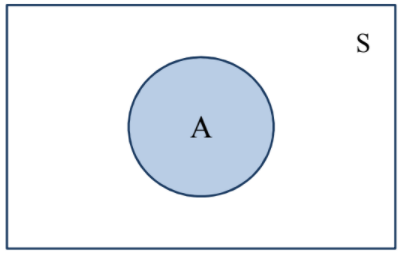
\includegraphics[width=0.5\linewidth]{images/screening/himpunan} 

}

\caption{Definisi ruang sampel dan anggota sampel}\label{fig:unnamed-chunk-2}
\end{figure}

Gambar di atas memberikan ilustrasi mengenai konsep ruang sampel dan anggota sampel. Pada gambar, \emph{event} A merupakan anggota dari ruang sampel \emph{S}. Konsep probabilitas erat kaitannya dengan konsep frekuensi relatif. Jika suatu eksperimen diulang sebanyak n kali, kemudian dicatat banyaknya jumlah keluaran dari \emph{n} jumlah eksperimen yang berupa \emph{event A}, maka frekuensi dari \emph{event A}, disimbolkan \emph{N}(\emph{A}), didefinisikan sebagai berikut. \[N(A)=\frac{banyaknya\ keluaran\ event\ A}{n}...(1)\]
Frekuensi relatif \emph{event} A dinyatakan sebagai frekuensi \emph{event} A dibagi banyaknya jumlah sampel \emph{n}. \[frekuensi\ relatif\ (A)=\frac{N(A)}{n}...(2)\]
Nilai frekuensi relatif suatu \emph{event} bergantung pada jumlah sampel n.~Semakin banyak n, maka nilai frekuensi relatif akan semakin stabil. Probabilitas suatu \emph{event} bersesuaian dengan nilai stabil dari frekuensi relatif \emph{event} tersebut. \textbf{Probabilitas suatu \emph{event} didefinisikan sebagai proporsi kemunculan suatu \emph{event} dari total \emph{n} jumlah random eksperimen}. Probabilitas kemunculan atau kejadian suatu \emph{event} disimbolkan P(\emph{event}). Maka, probabilitas kejadian \emph{event} A dalam ruang sampel S disimbolkan dengan P(A). Dua aturan dasar terkait teori probabilitas adalah probabilitas suatu \emph{event} tidak pernah bernilai negatif, dan probabilitas dari ruang sampel \emph{S} adalah 1.

~

\hypertarget{distribusi-probabilitas-kontinu}{%
\subsubsection{Distribusi Probabilitas Kontinu}\label{distribusi-probabilitas-kontinu}}

Seperti yang telah dijelaskan sebelumnya, probabilitas dapat didefinisikan sebagai peluang terjadinya suatu \emph{event} atau peluang kemunculan suatu nilai dari suatu eksperimen. Eksperimen yang dimaksud di sini adalah \textbf{\emph{ekperimen statistik}}, yaitu suatu proses yang menghasilkan data atau nilai numerik. Nilai probabilitas berada diantara 0 dan 1. Jika terdapat sekumpulan nilai, dan masing-masing nilai tersebut dikaitkan dengan probabilitas kejadiannya, maka akan diperoleh distribusi probabilitas.

Distribusi probabilitas dapat dibagi menjadi dua, yaitu distribusi probabilitas diskrit dan distribusi probabilitas kontinu. Fungsi yang menjelaskan suatu distribusi probabilitas dari variabel random diskrit disebut sebagai \textbf{\emph{probability mass function}}, sedangkan fungsi yang menjelaskan suatu distribusi probabilitas dari variabel random kontinu disebut sebagai \textbf{\emph{probability density function}}. Karena parameter reservoir merupakan variable random kontinu, maka penjelasan akan ditekankan pada teori \emph{probability density function}.

\emph{Probability Density Funtion} (disingkat PDF) adalah suatu fungsi f(x) yang memberikan bentuk distribusi probabilitas dari suatu variabel random kontinu. Konsep PDF sangat penting karena dengan mengetahui PDF dari suatu parameter, maka bentuk distribusi probabilitas dari parameter tersebut akan dapat diketahui. Misalkan, untuk parameter porositas reservoir, dengan mengetahui PDF dari porositas reservoir maka bentuk distribusi dari porositas akan diketahui. Secara matematis, PDF didefinisikan oleh persamaan berikut.\[P(a<X<b)=\int_a^{b}f(x)dx\]
Beberapa sifat dari PDF adalah sebagai berikut:

\begin{enumerate}
\def\labelenumi{\arabic{enumi}.}
\tightlist
\item
  f(x) \textgreater{} 0, x \(\in\) S. Maksud dari simbol ini adalah PDF \emph{f} selalu bernilai positif, dimana variabel random \emph{x} merupakan anggota dari ruang sampel \emph{S}.
\item
  \(\int_s f(x)dx=1\). Maksudnya adalah total luas daerah di bawah kurva PDF selalu sama dengan 1, artinya nilai probabilitas total (untuk seluruh anggota ruang sampel \emph{S}) adalah 1.
\end{enumerate}

Informasi PDF dapat digunakan untuk mencari nilai rata-rata (\(\mu\)) dan \emph{variance} (\(\sigma^2\)) dari PDF tersebut. Nilai rata-rata (\(\mu\)) dan \emph{variance} (\(\sigma^2\)) dapat dihitung menggunakan persamaan berikut.\[\mu=\int_s xf(x)dx\] \[\sigma^2=\int_s (x-\mu)^2f(x)dx=\int_s x^2f(x)dx-\mu^2...(3)\]
Terdapat beberapa bentuk distribusi kontinu yang akan digunakan dalam analisis EOR \emph{screening.} Berikut akan dijelaskan empat bentuk distribusi kontinu yang akan digunakan dalam algoritma EOR \emph{screening}.

~

\hypertarget{distribusi-normal-dan-standard-normal}{%
\subsubsection{Distribusi Normal dan Standard Normal}\label{distribusi-normal-dan-standard-normal}}

\textbf{Distribusi normal} (disebut juga \textbf{distribusi \emph{Gaussian}}) merupakan distribusi dari variabel random kontinu yang berbentuk mirip lonceng (``\emph{bell-shaped}''). Distribusi normal didefinisikan oleh dua parameter, yaitu nilai rata-rata (\(\mu\)) dan standard deviasi (\(\sigma\)).

\begin{figure}

{\centering 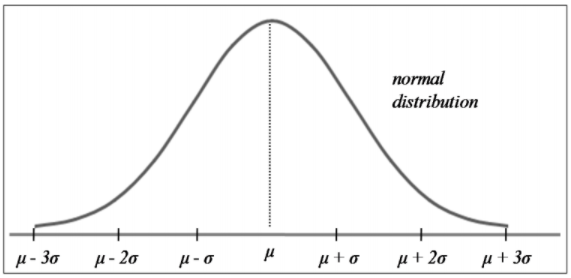
\includegraphics[width=0.5\linewidth]{images/screening/distribusi_normal} 

}

\caption{Bentuk distribusi normal}\label{fig:unnamed-chunk-3}
\end{figure}

Beberapa sifat dari distribusi normal adalah:
1. Kurva distribusi normal berbentuk mirip lonceng (``\_bell-shape\_d'') dengan titik puncak kurva berada di atas nilai rata-rata (\(\mu\)),
2. Kurva distribusi normal berbentuk simetri melalui nilai rata-rata (\(\mu\)), dan
3. Kurva distribusi normal semakin mendekati sumbu horizontal namun tidak pernah menyentuh atau melewati sumbu horizontal.

Hal yang terpenting dari kurva distribusi normal adalah luas daerah di bawah kurva distribusi normal. Hal ini penting karena luas daerah di bawah kurva distribusi normal pada suatu interval tertentu menyatakan \textbf{probabilitas} suatu nilai berada pada interval tersebut. Sama seperti aturan distribusi probabilitas untuk semua distribusi probabilitas kontinu yang telah dijelaskan sebelumnya, total luas daerah di bawah kurva distribusi normal adalah 1. Gambar berikut memperlihatkan konsep ini.

\begin{figure}

{\centering 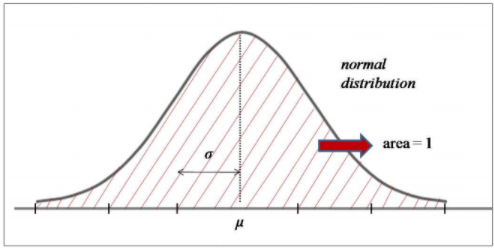
\includegraphics[width=0.5\linewidth]{images/screening/distribusi_normal_1} 

}

\caption{Total luas daerah di bawah kurva distribusi normal adalah 1}\label{fig:unnamed-chunk-4}
\end{figure}

\begin{figure}

{\centering 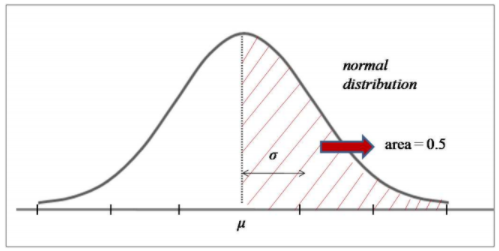
\includegraphics[width=0.5\linewidth]{images/screening/distribusi_normal_0.5} 

}

\caption{Total luas daerah setengah dari total distribusi normal adalah 0.5}\label{fig:unnamed-chunk-5}
\end{figure}

Maka, dengan mengetahui luas daerah di bawah kurva distribusi normal dalam suatu interval, probabilitas suatu nilai ada di dalam interval tersebut dapat diketahui. Hal lain yang perlu diketahui dari kurva distribusi normal adalah sebagai berikut:

\begin{enumerate}
\def\labelenumi{\arabic{enumi}.}
\tightlist
\item
  Sekitar 68.2\% dari luas daerah di bawah kurva distribusi normal berada dalam interval satu
  standard deviasi dari nilai rata-ratanya, yaitu \(\mu\) + \(\sigma\) dan \(\mu\) -- \(\sigma\),
\item
  Sekitar 95.4\% dari luas daerah di bawah kurva distribusi normal berada dalam interval dua
  standard deviasi dari nilai rata-ratanya, yaitu \(\mu\) + 2\(\sigma\) dan \(\mu\) -- 2\(\sigma\), dan
\item
  Sekitar 99.7\% dari luas daerah di bawah kurva distribusi normal berada dalam interval tiga
  standard deviasi dari nilai rata-ratanya, yaitu \(\mu\) + 3\(\sigma\) dan \(\mu\) -- 3\(\sigma\).
\end{enumerate}

Dengan kata lain, suatu nilai yang merupakan anggota dari populasi nilai distribusi normal yang bersangkutan akan berada pada \emph{range} ± 3 standard deviasi dari \emph{mean} \(\mu\). Karena hampir seluruh nilai yang merupakan anggota populasi berada pada \emph{range} ± 3 standard deviasi dari μ (dengan probabilitas 99.7\%), maka dapat disimpulkan bahwa suatu nilai yang berada di luar \emph{range} ± 3 standard deviasi dari \(\mu\) bukan merupakan anggota dari populasi yang bersangkutan (probabilitas nilai ini merupakan anggota dari populasi terkait sangat kecil, yaitu 100\% - 99.7\% = 0.3\%).

\begin{figure}

{\centering 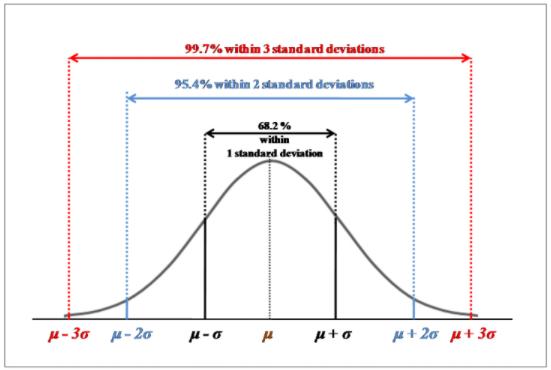
\includegraphics[width=0.5\linewidth]{images/screening/distribusi_normal_range} 

}

\caption{Luas daerah (probabilitas) di bawah kurva distribusi normal untuk masing-masing range standard deviasi dari mean}\label{fig:unnamed-chunk-6}
\end{figure}

\emph{
Probability Density Function} (PDF) distribusi normal diberikan oleh persamaan berikut. \[f(x)=\frac{1}{\sigma\sqrt{2\pi}}e^{-\frac{(x-\mu)^2}{2\sigma^2}}...(4)\]

Menentukan luas daerah di bawah kurva distribusi normal tidaklah selalu mudah karena masing- masing distribusi normal memiliki nilai rata-rata \(\mu\) dan standard deviasi \(\sigma\) yang berbeda satu sama lain. Oleh karena itu, digunakanlah teori \textbf{distribusi standard normal} untuk mempermudah menghitung luas daerah di bawah kurva distribusi normal. Prosedur dalam menentukan luas daerah di bawah kurva normal adalah mentransformasi nilai \emph{x} pada distribusi normal original menjadi nilai \emph{z} pada distribusi standard normal. Statistik \emph{z} disebut sebagai statistik standard normal, yaitu suatu parameter yang mengkarakterisasi nilai distribusi standard normal. Kemudian, luas daerah di bawah kurva standard normal ditentukan dengan melihat tabel luas daerah kurva standard normal yang telah disusun oleh para ahli statistik.
s
Konsep untuk mentransformasi kurva distribusi normal menjadi kurva standard normal adalah dengan menghitung berapa standard deviasi jauhnya suatu nilai x pada distribusi normal dari \emph{mean}-nya. Setelah hal ini diketahui, maka nilai \emph{x} dikonversi menjadi nilai \emph{z} menggunakan persamaan berikut. \[z=\frac{x-\mu}{\sigma}...(5)\]

Distribusi normal \emph{original} kini telah ditransformasi ke dalam distribusi standard normal dengan variabel \emph{z}. Distribusi standard normal dicirikan dengan nilai rata-rata \(\mu\) = 0 dan standard deviasi \(\sigma\) = 1. Luas daerah (probabilitas) suatu nilai standard normal akan jatuh pada interval 0 dan \emph{z} diperoleh dari kurva standard normal. Distribusi standard normal sangat berguna karena dapat mempermudah perhitungan probabilitas suatu nilai dalam distribusi normal.

~

\hypertarget{distribusi-segitiga-triangular}{%
\subsubsection{Distribusi Segitiga (Triangular)}\label{distribusi-segitiga-triangular}}

Distribusi segitiga merupakan bentuk distribusi kontinu yang dikarakterisasi oleh tiga titik, yaitu titik ujung bawah a, titik ujung atas b, dan titik tengah c, dimana a \textless{} b dan a ≤ c ≤ b.

\begin{figure}

{\centering 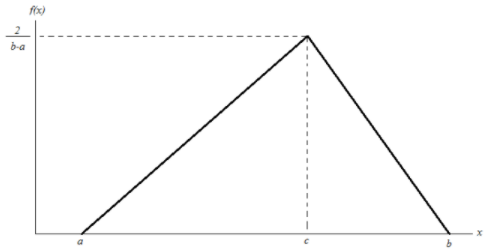
\includegraphics[width=0.5\linewidth]{images/screening/distribusi_segitiga} 

}

\caption{Distribusi segitiga}\label{fig:unnamed-chunk-7}
\end{figure}

\emph{Probability Density Function} (PDF) untuk distribusi segitiga diberikan oleh:

\[
f(x) =
\begin{cases}
  0,\ untuk\ x < a\ dan\ x > b\\ 
  \frac{2(x-a)}{(b-a)(c-a)},\ untuk\ a \leq x \leq c \\
  \frac{2(b-x)}{(b-a)(b-c)},\ untuk\ c \leq x \leq b
\end{cases}       
\]

~

\hypertarget{distribusi-uniform}{%
\subsubsection{Distribusi Uniform}\label{distribusi-uniform}}

Distribusi \emph{uniform} kontinu adalah bentuk distribusi dimana setiap anggota distribusi memiliki probabilitas kemunculan yang sama. Bentuk distribusi ini dicirikan oleh dua parameter, yaitu nilai minimum \emph{a}, dan nilai maksimum \emph{b}. \emph{Probability Density Function} (PDF) dari distribusi \emph{uniform} adalah:

\[
f(x)=
\begin{cases}
  \frac{1}{b-a},\ untuk\ a \leq x \leq b\\
  0,\ untuk\ x > a\ atau\ x > b
\end{cases}
\]

\begin{figure}

{\centering 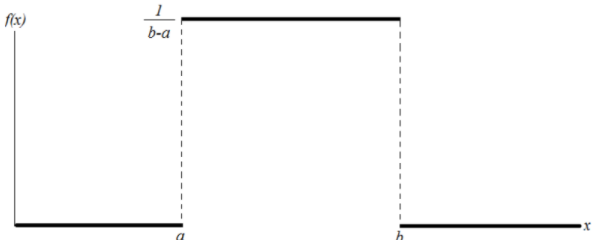
\includegraphics[width=0.5\linewidth]{images/screening/distribusi_uniform} 

}

\caption{Distribusi uniform}\label{fig:unnamed-chunk-8}
\end{figure}

~

\hypertarget{distribusi-log-normal}{%
\subsubsection{Distribusi Log Normal}\label{distribusi-log-normal}}

Distribusi log normal berkaitan dengan distribusi normal, sehingga parameter-parameter distribusi log normal dapat dinyatakan dalam bentuk parameter distribusi normal. Misalkan Y adalah suatu variabel random kontinu yang terdistribusi normal, maka variabel random kontinu = D akan terdistribusi log normal dengan:

\emph{Mean} log normal = E{[}ln(X){]} = E(Y) = \(\mu\)

\emph{Variance} log normal = Var{[}ln(X){]} = Var{[}Y{]} = \(\sigma\)\textsuperscript{2}

dimana ln(X) = ln(e\textsuperscript{Y}) = Y

~

Bentuk distribusi log normal adalah seperti distribusi normal namun miring ke kiri. Hal ini disebabkan karena distribusi normal memiliki \emph{skewness} nol, sedangkan distribusi log normal memiliki \emph{skewness} positif.

\begin{figure}

{\centering 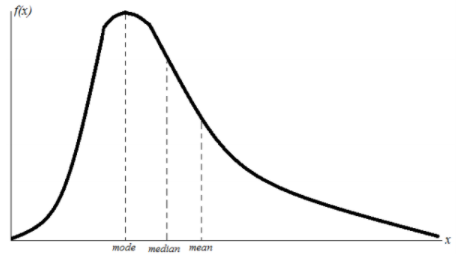
\includegraphics[width=0.5\linewidth]{images/screening/distribusi_log_normal} 

}

\caption{Distribusi log normal}\label{fig:unnamed-chunk-9}
\end{figure}

\emph{Mean} dan \emph{variance} dari variabel log normal \emph{X} adalah:
\[\mu_X = e^{(\mu+\frac{\sigma^2}{2})}\]
\[\sigma^2_X = (e^{2\mu+\sigma^2})(e^{\sigma^2}-1\]
Dimana \(\mu\) dan \(\sigma\)\textsuperscript{2} adalah \emph{mean} dan \emph{variance} dari variabel normal \emph{Y}. Terlihat bahwa \emph{mean} dan \emph{variance} dari variabel log normal adalah fungsi dari \emph{mean} dan \emph{variance} variabel normal. Karenadistribusi log normal dan distribusi normal saling berkaitan, maka \emph{Probability Density Function} (PDF) dari distribusi log normal dinyatakan oleh parameter-parameter distribusi normal.
\[f(x) = \frac{1}{x\sigma\sqrt{2\pi}}\ exp\ [-\frac{1}{2\sigma^2}(ln\ x-\mu)^2]\]
Pada persamaan (8) di atas, \(\mu\) dan \(\sigma\)\textsuperscript{2} adalah \emph{mean} dan \emph{variance} dari variabel normal \emph{Y}.

\hypertarget{metode-numerik}{%
\subsection{Metode Numerik}\label{metode-numerik}}

Dalam aplikasi, seringkali dijumpai permasalahan berupa penentuan akar (solusi) dari sebuah persamaan \emph{f(x)} = 0. Jika \emph{f(x)} adalah suatu fungsi sederhana, tentu solusinya akan mudah diperoleh secara eksak. Permasalahan timbul apabila fungsi \emph{f(x)} adalah suatu fungsi kompleks yang solusinya tidak dapat diperoleh secara eksak. Untuk kasus-kasus dimana solusi dari fungsi \emph{f(x)} tidak dapat diperoleh secara eksak, dilakukan pendekatan pencarian solusi secara numerik, yaitu dilakukan perubahan solusi secara bertahap dengan sedikit demi sedikit menambah tingkat ketelitian sampai diperoleh solusi dengan tingkat ketelitian yang diinginkan. Metode mencarisolusi seperti ini disebut sebagai \textbf{metode approksimasi berurutan \emph{(method of successive approximation)}} atau disebut juga dengan \textbf{metode iterasi}. Metode iterasi tidak hanya harus diterapkan pada kasus-kasus yang tidak memiliki solusi eksak. Kasus-kasus sederhana yang solusi eksaknya ada pun dapat dicari pendekatan solusinya menggunakan metode iterasi. Bahkan, metode iterasi lebih disukai untuk digunakan di kasus-kasus sederhana oleh banyak orang karena metode ini kadang lebih mudah diterapkan dibandingkan mencari solusi eksak secara analitik.

Terdapat beberapa metode iterasi yang dapat digunakan untuk mencari solusi. Pada penelitian ini, metode iterasi yang digunakan adalah metode Newton-Raphson. Oleh karena itu, pada subbab ini, penjelasan metode numerik dibatasi pada metode Newton-Raphson.

\textbf{Metode Newton-Raphson}, yang juga sering disebut sebagai \textbf{metode Newton} adalah suatu metode numerik yang melibatkan turunan pertama dari fungsi \emph{f(x)} dalam proses iterasi. Pada penelitian ini, metode Newton digunakan untuk mencari titik potong antara dua kurva distribusi, yaitu kurva distribusi \emph{database} dan kurva distribusi \emph{input}. Jika distribusi \emph{database} memiliki \emph{density function} \emph{f(x)} dan distribusi \emph{input} memiliki \emph{density function} \emph{g(x)}, maka fungsi \emph{h(x)} = \emph{f(x)} - \emph{g(x)} menyatakan selisih antara \emph{density database} dengan \emph{density input}. Nilai fungsi \emph{h(x)} = 0 menyatakan titik potong antara kedua kurva \emph{f(x)} dan \emph{g(x)}. Metode Newton diterapkan terhadap fungsi \emph{h(x)} untuk mencari pendekatan solusi \emph{h(x)} = 0. Hasil dari penerapan metode Newton adalah diperolehnya pendekatan nilai x dimana \emph{h(x)} sangat dekat ke nol. Nilai x ini merupakan titik potong yang dicari.

\begin{figure}

{\centering 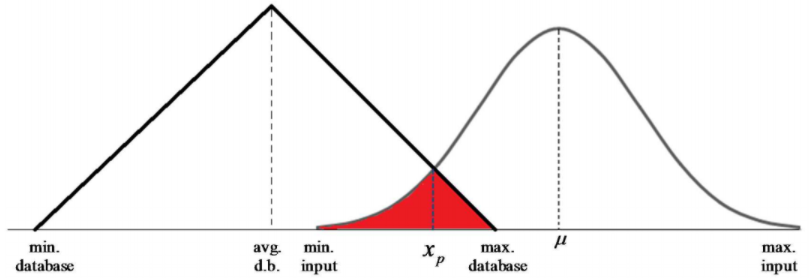
\includegraphics[width=0.5\linewidth]{images/screening/newton_rhapson} 

}

\caption{Titik x~p~ merupakan titik potong antara kurva distribusi database dengan kurva distribusi input. Titik potong ini dicari menggunakan metode Newton-Rhapson}\label{fig:unnamed-chunk-10}
\end{figure}

Misalkan \emph{h(x)} adalah fungsi yang dapat didiferensialkan dan misalkan x\textsubscript{1} adalah tebakan awal solusi untuk \emph{h(x)} = 0. Jika E melambangkan batas toleransi error dari solusi, maka metode Newton diterapkan dengan mengulangi langkah berikut untuk n = 1, 2 \ldots{} sampai diperoleh \textbar x\textsubscript{n+1} - x\textsubscript{n}\textbar{} \textless{} \emph{E}:
\[x_{n+1} = x_n - \frac{h(x_n)}{h'(x_n)}...(9)\]
Persamaan (9) di atas merupakan prosedur perulangan (iterasi) untuk mencari solusi x yang sangat mendekati \emph{h(x)} = 0. Prosedur iterasi dilakukan sampai dicapai suatu nilai konvergen (yang kemudian diambil sebagai solusi), atau sampai suatu batas \emph{error} tertentu \emph{E}, dimana \emph{E} = \textbar x\textsubscript{n+1} - x\textsubscript{n}\textbar{} Hal yang perlu diperhatikan dalam penggunaan metode Newton-Raphson adalah pemilihan tebakan awal untuk solusi. Permasalahan yang sering timbul adalah pemilihan tebakan awal yang terlalu jauh sehingga kekonvergenan lambat diperoleh, atau bahkan solusi konvergen tidak dapat diperoleh.

Setelah titik potong dari dua kurva distribusi diperoleh dari metode Newton, maka langkah selanjutnya adalah mencari luas daerah irisan dari kedua kurva distribusi tersebut (arsiran merah pada Gambar 9). Luas daerah irisan ini menyatakan probabilitas kecocokan distribusi \emph{input} terhadap distribusi \emph{database}.

Penentuan luas daerah irisan melibatkan penggunaan integral dari fungsi distribusi dalam suatu interval {[}\emph{a}, \emph{b}{]}. Metode numerik yang digunakan dalam penentuan luas daerah (integral) adalah \textbf{metode Simpson} (disebut juga \textbf{metode Parabolik}). Metode Simpson mencari pendekatan terhadap luas daerah dari suatu bangun ruang dengan membagi interval {[}\emph{a}, \emph{b}{]} ke dalam n jumlah sub-interval (\emph{n} harus genap), dimana pada masing-masing sub-interval ditempatkan suatu bangun ruang parabola. Sehingga, akan terdapat \emph{n} buah parabola di bawah suatu kurva \emph{f(x)}. Luas daerah di bawah kurva \emph{f(x)} dapat didekati dengan menjumlahkan seluruh n buah parabola dalam interval {[}\emph{a}, \emph{b}{]}.

Metode Simpson dinyatakan sebagai berikut.
\[\int_a^bf(x)dx \approx \frac{h}{3}[f(x_0)+4f(x_1)+2f(x_2)+...+4f(x_{n-1})+f(x_n)]...(10)\]
Pada persamaan (10) di atas, h adalah lebar sub-interval dan nilai-nilai 1, 4, 2, 4, 2, 4, 2,\ldots, 2, 4, 1 adalah koefisien-koefisien yang terkait dengan setiap suku \emph{f(x)}.

~

\hypertarget{metode-analisis-eor-screening}{%
\section{Metode Analisis EOR Screening}\label{metode-analisis-eor-screening}}

Teori dasar yang telah dijelaskan di subbab pertamaS merupakan dasar yang akan digunakan untuk analisis EOR \emph{screening} dalam subbab ini. Seperti yang telah disebutkan pada bagian pendahuluan, analisis dilakukan untuk mengetahui probabilitas kecocokan dari setiap parameter \emph{input} reservoir (untuk setiap metode EOR) terhadap \emph{database}. \emph{Database} ini berupa interval nilai parameter reservoir untuk setiap metode EOR yang telah berhasil diterapkan di seluruh dunia. \emph{Database} yang digunakan diambil dari paper Aladasani dan Baojun Bai (2010). Tabel berikut memperlihatkan \emph{database} yang digunakan untuk EOR \emph{screening}.

\begin{center}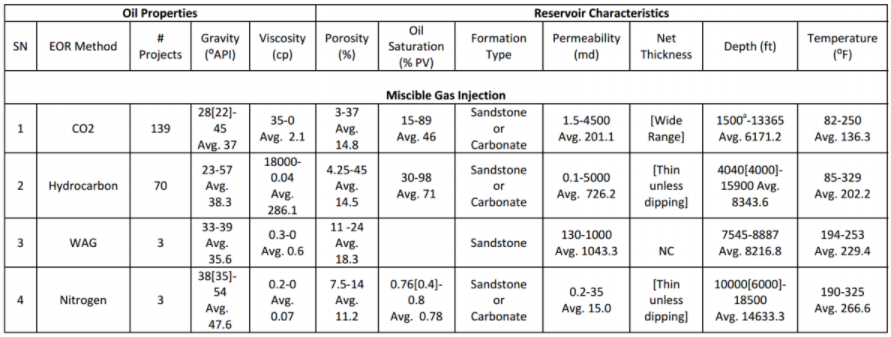
\includegraphics[width=1\linewidth]{images/screening/miscible} \end{center}

\begin{center}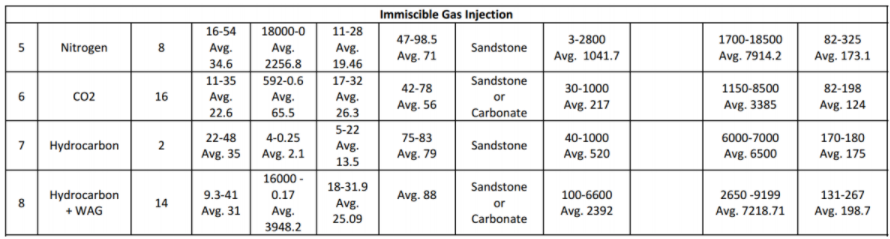
\includegraphics[width=1\linewidth]{images/screening/immiscible} \end{center}

\begin{center}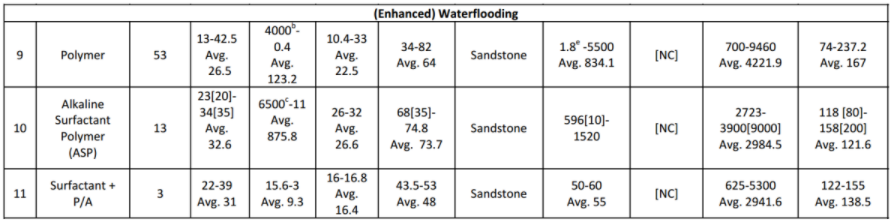
\includegraphics[width=1\linewidth]{images/screening/waterflooding} \end{center}

\begin{center}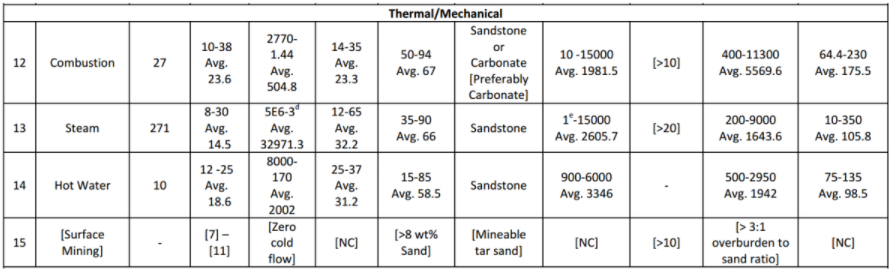
\includegraphics[width=1\linewidth]{images/screening/thermal} \end{center}

\textbackslash begin\{figure\}

\{\centering 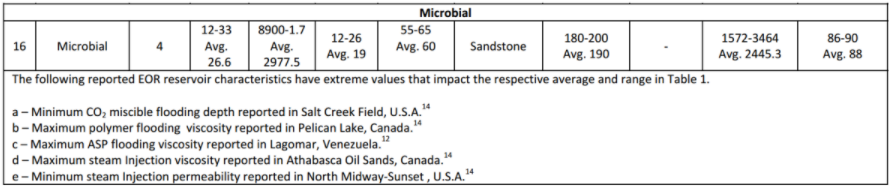
\includegraphics[width=1\linewidth]{images/screening/microbial}

\}

\textbackslash caption\{\emph{Range} nilai dari beberapa parameter reservoir terhadap setiap metode EOR yang telah sukses diterapkan di beberapa tempat di seluruh dunia. \emph{Range} nilai ini akan dijadikan data acuan dalam analisis statistik. (Sumber: Ahmad Aladasani nad Baojun Bai, 2010, \emph{Recent Developments and Updated Screening Criteria of Enhanced Oil Recovery Techniques}, SPE Paper 130726)\}\label{fig:unnamed-chunk-15}
\textbackslash end\{figure\}

Interval nilai parameter reservoir yang tertera di Gambar 10 akan digunakan sebagai acuan \emph{database} dalam analisis. Metode analisis EOR \emph{screening} terbagi atas \textbf{metode analisis untuk \emph{input} data \emph{single-value}} dan \textbf{metode analisis untuk \emph{input} data distribusi}. Berikut akan dijelaskan kedua metode analisis ini.

\hypertarget{metode-analisis-eor-screening-untuk-input-data-single-value}{%
\subsection{Metode Analisis EOR Screening Untuk Input Data Single-Value}\label{metode-analisis-eor-screening-untuk-input-data-single-value}}

\emph{Input} data \emph{single-value} yang dimaksud di sini adalah parameter \emph{input} berupa nilai tunggal, misalnya \emph{input} porositas berupa satu nilai porositas yang mewakili distribusi porositas. Terdapat dua algoritma yang digunakan dalam EOR \emph{screening}, yaitu algoritma normal dan algoritma \emph{tight}. Bentuk distribusi probabilitas yang digunakan dalam analisis input data single value adalah distribusi segitiga.

\hypertarget{algoritma-normal-normal-screening-algorithm}{%
\subsubsection{Algoritma Normal (Normal Screening Algorithm)}\label{algoritma-normal-normal-screening-algorithm}}

Algoritma normal yang digunakan dalam EOR screening dibagi menjadi dua, yaitu \textbf{algoritma statistik (\emph{statistics algorithm})} dan \textbf{algoritma teknik (\emph{engineering algorithm})}. Algoritma statistik adalah algoritma yang murni menggunakan konsep statistik dalam penentuan kriteria \emph{screen}ing, sedangkan algoritma teknik adalah algoritma yang menyertakan faktor \emph{engineering sense} ke dalam perhitungan \emph{screening}.

Pada kedua algoritma, disertakan parameter \textbf{\emph{cut-off}}. Parameter \emph{cut-off} menyatakan tambahan data (berupa luas daerah) sebesar ±\(\alpha\)\% dari distribusi data original. Parameter ini memungkinkan \emph{user} untuk menentukan nilai probabilitas (sebesar \(\alpha\)\%) saat parameter input \emph{x} tepat jatuh di nilai maksimum atau nilai minimum \emph{database}.
\textbackslash begin\{figure\}

\{\centering 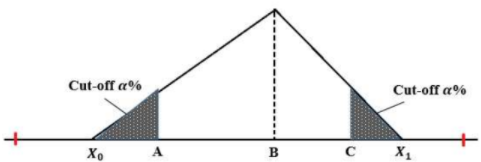
\includegraphics[width=0.5\linewidth]{images/screening/cut-off}

\}

\textbackslash caption\{Konsep \emph{cut-off} dalam algoritma EOR \emph{screening}\}\label{fig:unnamed-chunk-16}
\textbackslash end\{figure\}

~

\textbf{a. Algoritma Statistik (Statistics Algoritm)}
Pada algoritma statistik, nilai rata-rata (\emph{mean}) dari distribusi \emph{database} digunakan sebagai acuan penentuan kecocokan 100\% terhadap suatu metode EOR.

\begin{figure}

{\centering 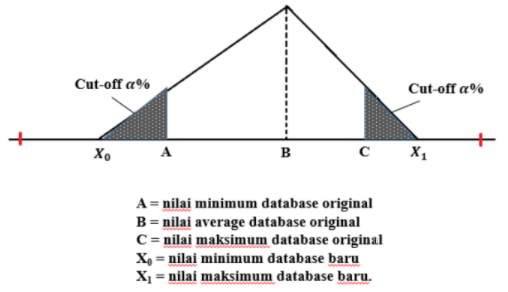
\includegraphics[width=0.5\linewidth]{images/screening/algoritma_statistik} 

}

\caption{Konsep algoritma statistik}\label{fig:unnamed-chunk-17}
\end{figure}

Berdasarkan \emph{database}, maka variable yang diketahui nilainya adalah A, B, dan C (mengacu pada gambar di atas). X\textsubscript{0} dan X\textsubscript{1} merupakan dua variabel \emph{unknown} yang harus dicari nilainya. Penentuan nilai X\textsubscript{0} adalah sebagai berikut.
\textbackslash begin\{figure\}

\{\centering 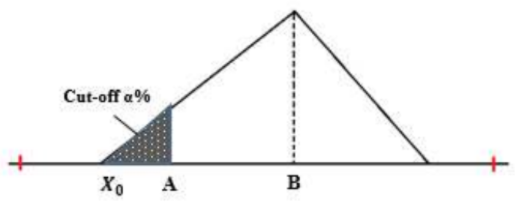
\includegraphics[width=0.5\linewidth]{images/screening/X0}

\}

\textbackslash caption\{Konsep penentuan \textbf{X\textsubscript{0}}\}\label{fig:unnamed-chunk-18}
\textbackslash end\{figure\}
\[X_0 = \frac{-b\ ±\ \sqrt{D} }{2a}...(11)\]
Dimana:
D = b\textsuperscript{2} - 4a
a = 1 - 2P
b = 4BP - 2A
c = A\textsuperscript{2} - 2PB\textsuperscript{2}
A = nilai minimum dari \emph{database original}
B = nilai rata-rata (\emph{mean}) dari \emph{database original}
P = probabilitas nilai di x = \emph{A} (nyatakan P = \(\frac{\alpha}{100}\)).
Solusi X\textsubscript{0} yang dipilih adalah yang memenuhi X\textsubscript{0} \textless{} A

Penentuan nilai X\textsubscript{1} adalah sebagai berikut.
\textbackslash begin\{figure\}

\{\centering 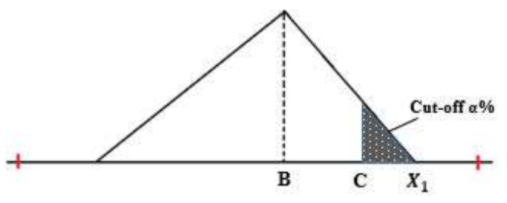
\includegraphics[width=0.5\linewidth]{images/screening/X1}

\}

\textbackslash caption\{Konsep penentuan \textbf{X\textsubscript{1}}\}\label{fig:unnamed-chunk-19}
\textbackslash end\{figure\}
\[X_1 = \frac{-b\ ±\ \sqrt{D} }{2a}...(12)\]
Dimana:
D = b\textsuperscript{2} - 4a
a = 1 - 2P
b = 4BP - 2C
c = C\textsuperscript{2} - 2PB\textsuperscript{2}
A = nilai maksimum dari \emph{database original}
B = nilai rata-rata (\emph{mean}) dari \emph{database original}
P = probabilitas nilai di x = \emph{C} (nyatakan P = \(\frac{\alpha}{100}\)).
Solusi X\textsubscript{1} yang dipilih adalah yang memenuhi X\textsubscript{1} \textgreater{} A

Setelah nilai X\textsubscript{0} dan X\textsubscript{1} diperoleh, maka langkah selanjutnya adalah menentukan probabilitas kecocokan. Probabilitas kecocokan suatu parameter input \emph{x} terhadap \emph{database} (dinyatakan oleh P(\emph{x}) adalah sebagai berikut.

\begin{itemize}
\tightlist
\item
  Untuk parameter \emph{input} di bawah nilai \emph{mean} dari \emph{database original} (x \textless{} B)
  \textbackslash begin\{figure\}
\end{itemize}

\{\centering 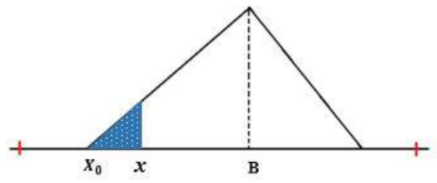
\includegraphics[width=0.5\linewidth]{images/screening/kecilB}

\}

\caption{Perhitungan P(x) untuk nilai input x < B}

\label{fig:unnamed-chunk-20}
\textbackslash end\{figure\}
\[P(x) = \left( \frac{1}{2}\frac{(x-X_0)^2}{(B-X_0)^2} \right) \times 2\  ...(13)\]
Dimana:
\emph{x} = nilai parameter \emph{input single value}
\emph{X\textsubscript{0}} = nilai minimum \emph{database} baru
\emph{B} = nilai \emph{mean database original}

\begin{itemize}
\tightlist
\item
  Untuk parameter \emph{input} di bawah nilai \emph{mean} dari \emph{database original} (x \textgreater{} B)
  \textbackslash begin\{figure\}
\end{itemize}

\{\centering 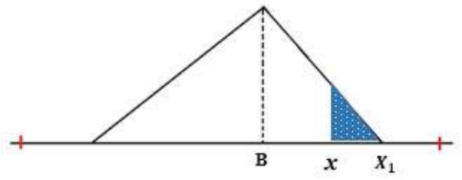
\includegraphics[width=0.5\linewidth]{images/screening/besarB}

\}

\caption{Perhitungan P(x) untuk nilai input x > B}

\label{fig:unnamed-chunk-21}
\textbackslash end\{figure\}
\[P(x) = \left( \frac{1}{2}\frac{(X_0-x)^2}{(X_1-B)^2} \right) \times 2\  ...(14)\]
Dimana:
\emph{x} = nilai parameter \emph{input single value}
\emph{X\textsubscript{1}} = nilai maksimum \emph{database} baru
\emph{B} = nilai \emph{mean database original}

~

\textbf{b. Algoritma Teknik (Engineering Algoritm)}
Pada algoritma teknik, terdapat tiga tipe algoritma yang dapat dipilih oleh \emph{user}, yaitu algoritma tipe \emph{average}, algoritma tipe maksimum, dan algoritma tipe minimum.

~

\textbf{(1) Algoritma Teknik Tipe \emph{Average}}
Algoritma tipe ini adalah algoritma yang sama dengan yang diterapkan pada algoritma statistik, dimana mean dari \emph{database} dijadikan titik acuan penentuan kecocokan 100\%.
\textbackslash begin\{figure\}

\{\centering 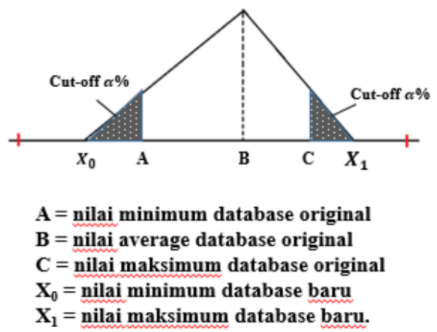
\includegraphics[width=0.5\linewidth]{images/screening/tipe_average}

\}

\textbackslash caption\{Konsep algoritma teknik tipe \emph{average}\}\label{fig:unnamed-chunk-22}
\textbackslash end\{figure\}

~

\textbf{(2) Algoritma Teknik Tipe Minimum}
Algoritma tipe ini menetapkan nilai kecocokan 100\% untuk nilai parameter \emph{input} di bawah nilai \emph{mean database original}. Bentuk distribusi data yang digunakan adalah sebagai berikut.

\begin{figure}

{\centering 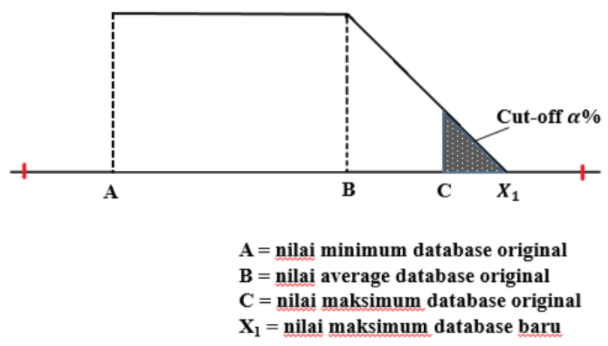
\includegraphics[width=0.5\linewidth]{images/screening/tipe_minimum} 

}

\caption{Konsep algoritma teknik tipe minimum}\label{fig:unnamed-chunk-23}
\end{figure}

Langkah pertama dari algoritma adalah mencari nilai X\textsubscript{1}. Nilai X\textsubscript{1} ditentukan sebagai berikut.
\[X_1 = \frac{-b\ ±\ \sqrt{D} }{2a}...(15)\]
Dimana:
D = b\textsuperscript{2} - 4a
a = 1 - P
b = 4BP - 2C
c = C\textsuperscript{2} - 2PB\textsuperscript{2}
A = nilai maksimum dari \emph{database original}
B = nilai rata-rata (\emph{mean}) dari \emph{database original}
P = probabilitas nilai di x = \emph{C} (nyatakan P = \(\frac{\alpha}{100}\)).
Solusi X\textsubscript{1} yang dipilih adalah yang memenuhi X\textsubscript{1} \textgreater{} C

Setelah nilai X\textsubscript{1} diperoleh, maka langkah selanjutnya adalah menentukan probabilitas kecocokan. Probabilitas kecocokan suatu parameter input \emph{x} terhadap \emph{database} (dinyatakan oleh P(\emph{x})) adalah sebagai berikut.

\begin{itemize}
\tightlist
\item
  Untuk parameter \emph{input} di atas nilai \emph{mean} dari \emph{database original} (x \textgreater{} B)
  \textbackslash begin\{figure\}
\end{itemize}

\{\centering 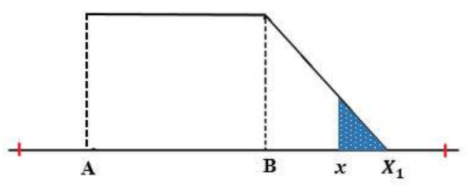
\includegraphics[width=0.5\linewidth]{images/screening/besarB1}

\}

\caption{Perhitungan P(x) untuk nilai input x > B}

\label{fig:unnamed-chunk-24}
\textbackslash end\{figure\}
\[P(x) = \left[\frac{(X_1-x)^2}{(X_1-B)^2} \right]...(16)\]

~

\begin{itemize}
\tightlist
\item
  Untuk parameter \emph{input} di bawah nilai \emph{mean} dari \emph{database original} (x \textless{} B)
  \textbackslash begin\{figure\}
\end{itemize}

\{\centering 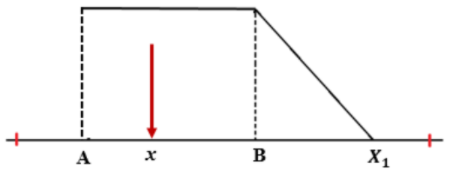
\includegraphics[width=0.5\linewidth]{images/screening/kecilB1}

\}

\caption{Perhitungan P(x) untuk nilai input x < B}

\label{fig:unnamed-chunk-25}
\textbackslash end\{figure\}
\[P(x) = 1...(17)\]

~

\textbf{(3) Algoritma Teknik Tipe Maksimum}
Algoritma tipe ini menetapkan nilai kecocokan 100\% untuk nilai parameter \emph{input} di atas nilai \emph{mean database original}. Bentuk distribusi data yang digunakan adalah sebagai berikut.

\begin{figure}

{\centering 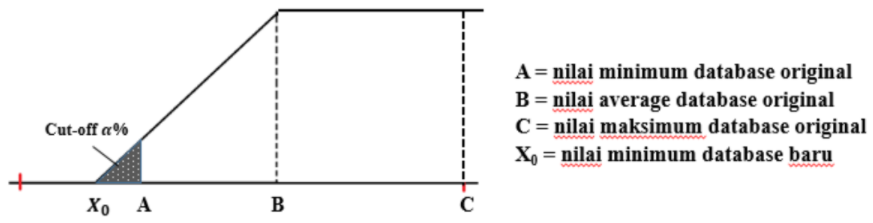
\includegraphics[width=0.5\linewidth]{images/screening/tipe_maksimum} 

}

\caption{Konsep algoritma teknik tipe maksimum}\label{fig:unnamed-chunk-26}
\end{figure}

Langkah pertama dari algoritma adalah mencari nilai X\textsubscript{0}. Nilai X\textsubscript{0} ditentukan sebagai berikut.
\[X_0 = \frac{-b\ ±\ \sqrt{D} }{2a}...(18)\]
Dimana:
D = b\textsuperscript{2} - 4a
a = 1 - P
b = 2BP - 2A
c = A\textsuperscript{2} - 2PB\textsuperscript{2}
A = nilai minimum dari \emph{database original}
B = nilai rata-rata (\emph{mean}) dari \emph{database original}
P = probabilitas nilai di x = \emph{A} (nyatakan P = \(\frac{\alpha}{100}\)).
Solusi X\textsubscript{0} yang dipilih adalah yang memenuhi X\textsubscript{0} \textless{} A.

Setelah nilai X\textsubscript{0} diperoleh, maka langkah selanjutnya adalah menentukan probabilitas kecocokan. Probabilitas kecocokan suatu parameter input x terhadap \emph{database} (dinyatakan oleh P(\emph{x})) adalah sebagai berikut.

\begin{itemize}
\tightlist
\item
  Untuk parameter \emph{input} di bawah nilai \emph{mean} dari \emph{database original} (x \textless{} B)
  \textbackslash begin\{figure\}
\end{itemize}

\{\centering 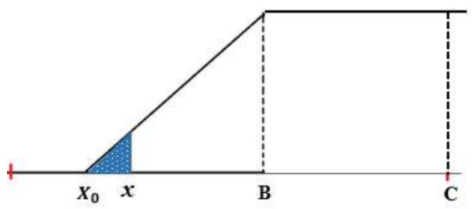
\includegraphics[width=0.5\linewidth]{images/screening/kecilB2}

\}

\caption{Perhitungan P(x) untuk nilai input x < B}

\label{fig:unnamed-chunk-27}
\textbackslash end\{figure\}
\[P(x) = \left[\frac{(x-X_0)^2}{(B-X_0)^2}\right] ...(19)\]

~

\begin{itemize}
\tightlist
\item
  Untuk parameter \emph{input} di atas nilai \emph{mean} dari \emph{database original} (x \textless{} B)
  \textbackslash begin\{figure\}
\end{itemize}

\{\centering 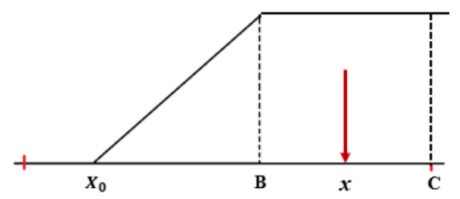
\includegraphics[width=0.5\linewidth]{images/screening/besarB2}

\}

\caption{Perhitungan P(x) untuk nilai input x > B}

\label{fig:unnamed-chunk-28}
\textbackslash end\{figure\}
\[P(x) = 1...(17)\]

~

\hypertarget{algoritma-tight-tight-screening-algorithm}{%
\subsubsection{\texorpdfstring{Algoritma \emph{Tight (Tight Screening Algorithm)}}{Algoritma Tight (Tight Screening Algorithm)}}\label{algoritma-tight-tight-screening-algorithm}}

Algoritma \emph{tight} diterapkan pada hasil (\emph{score}) algoritma normal. Algoritma ini menerapkan prosedur tambahan dalam perhitungan dengan cara mempertimbangkan banyak dan besarnya nilai \emph{unmatch} dari score algoritma normal, sehingga metode EOR yang memiliki nilai \emph{unmatch} akan mengalami perubahan peringkat sesuai dengan banyaknya jumlah nilai \emph{unmatch} dan besarnya nilai \emph{unmatch}.

Algoritma \emph{tight} diterapkan menggunakan sejumlah parameter berikut.

\textbf{Average Match and Unmatch Score} = \(\frac{Total\ Match\ Score\ +\ Total\ Unmatch\ Score}{Number\ of\ Match\ +\ Number\ of\ Unmatch}\)

\textbf{Average Match Score} = \(\frac{Total\ Match\ Score}{Number\ of\ Match}\)

\textbf{Ratio} = \(\frac{Average\ Match\ and\ Unmatch\ Score}{Average\ Match\ Score}\)

~

Score dari algoritma \emph{tight screening} dinyatakan oleh:

\textbf{Tight Screening Score} = \textbf{(Normal Screening Score)} \(\times\) Ratio \ldots{} (21)

~

\hypertarget{perhitungan-total-probabilitas-kecocokan}{%
\subsubsection{Perhitungan Total Probabilitas Kecocokan}\label{perhitungan-total-probabilitas-kecocokan}}

Total probabilitas kecocokan suatu metode EOR terhadap database dihitung menggunakan persamaan yang melibatkan hasil kali antara probabilitas kecocokan individu per parameter dengan nilai weighting factor. Persamaan ini berlaku baik pada algoritma statistik maupun algoritma teknik.
\[Probability\ (average\ score) = \frac{w_1F_1+w_2F_2+...+w_8F_8}{w_1+w_2+...+w_8}\]
\[Probability\ (average\ score) = \frac{\sum_{j=1}^{8}w_jF_j }{\sum_{j=1}^{8}w_j}...(22)\]
Dimana:
\emph{w\textsubscript{i}} = \emph{weighting factor} parameter ke-\emph{i}
\emph{F\textsubscript{i}} = parameter \emph{input} ke-\emph{i}

Metode EOR dengan nilai probabilitas kecocokan terbesar terhadap database akan dipilih sebagai \emph{the most probable EOR method} bagi reservoir target tersebut.

~

\hypertarget{algoritma-penalty-factor-dalam-eor-screening}{%
\subsubsection{\texorpdfstring{Algoritma \emph{Penalty Factor} Dalam EOR \emph{Screening}}{Algoritma Penalty Factor Dalam EOR Screening}}\label{algoritma-penalty-factor-dalam-eor-screening}}

Dalam EOR \emph{screening}, diterapkan algoritma tambahan untuk mengakomodasi \emph{input} \emph{user} yang berada di luar \emph{database.} Algoritma ini disebut dengan algoritma \emph{penalty} \emph{factor.} Algoritma \emph{penalty} \emph{factor} mengakomodasi seberapa jauh nilai \emph{input} \emph{user} yang berada di luar \emph{database.} Maka, semakin jauh nilai \emph{input} \emph{user} dari \emph{database}, nilai probabilitas total menjadi semakin kecil dan menurunkan peringkat metode EOR terkait dalam peringkat kecocokan. Algoritma \emph{penalty} \emph{factor} memberikan nilai kecocokan negatif.

Algoritma \emph{penalty} \emph{factor} diterapkan untuk setiap tipe algoritma \emph{screening} yang digunakan, termasuk algoritma screening tipe \emph{average}, maksimum, dan minimum. Persamaan-persamaan yang digunakan untuk setiap algoritma adalah sebagai berikut.

\textbf{a. Algoritma Tipe \emph{Average}}
Untuk algoritma tipe \emph{average}, \emph{penalty factor} diterapkan baik untuk kasus \emph{input user} di bawah minimum \emph{database} maupun untuk kasus \emph{input user} di atas maksimum \emph{database}.
\textbackslash begin\{figure\}

\{\centering 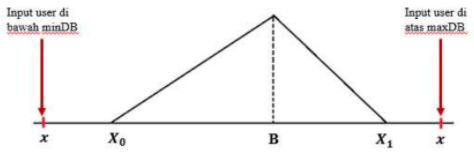
\includegraphics[width=0.5\linewidth]{images/screening/tipe_average1}

\}

\textbackslash caption\{\emph{Penalty factor} untuk algoritma tipe \emph{average}\}\label{fig:unnamed-chunk-29}
\textbackslash end\{figure\}

~

Untuk nilai input \textgreater{} nilai maksimum \emph{database},
\[Penalty\ Factor\ = \frac{maxDB\ -\ nilai\ input}{maxDB\ -\ minDB}...(23)\]
Untuk nilai input \textless{} nilai minimum \emph{database},
\[Penalty\ Factor\ = \frac{nilai\ input\ -\ minDB}{maxDB\ -\ minDB}...(24)\]

~

\_\_b. Algoritma Tipe Minimum
Untuk algoritma tipe minimum, \emph{penalty factor} diterapkan hanya untuk untuk kasus \emph{input user} yang berada di atas nilai maksimum \emph{database}.

\begin{figure}

{\centering 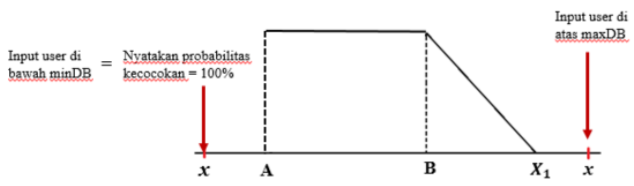
\includegraphics[width=0.5\linewidth]{images/screening/tipe_minimum1} 

}

\caption{*Penalty factor* untuk algoritma tipe minimum}\label{fig:unnamed-chunk-30}
\end{figure}

\[Penalty\ Factor\ = \frac{maxDB\ -\ nilai\ input}{maxDB\ -\ minDB}...(25)\]

~

\_\_b. Algoritma Tipe Maksimum
Untuk algoritma tipe minimum, \emph{penalty factor} diterapkan hanya untuk untuk kasus \emph{input user} yang berada di bawah nilai maksimum \emph{database}.

\begin{figure}

{\centering 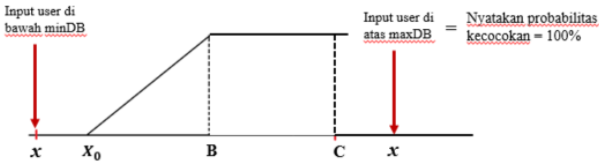
\includegraphics[width=0.5\linewidth]{images/screening/tipe_maksimum1} 

}

\caption{*Penalty factor* untuk algoritma tipe maksimum}\label{fig:unnamed-chunk-31}
\end{figure}

\[Penalty\ Factor\ = \frac{nilai\ input\ -\ minDB}{maxDB\ -\ minDB}...(26)\]

Sedangkan, untuk kasus \emph{input} distribusi, algoritma \emph{penalty factor} diterapkan sama seperti pada kasus \emph{input single value} untuk tipe algoritma \emph{average}.

~

\hypertarget{metode-analisis-eor-screening-untuk-input-data-distribusi}{%
\subsection{\texorpdfstring{Metode Analisis EOR \emph{Screening} Untuk \emph{Input} Data Distribusi}{Metode Analisis EOR Screening Untuk Input Data Distribusi}}\label{metode-analisis-eor-screening-untuk-input-data-distribusi}}

Untuk kasus \emph{input} data distribusi, maka \emph{input} dari \emph{user} berupa parameter-parameter dari distribusi \emph{input}, seperti \emph{mean}, standard deviasi, nilai minimum, dan nilai maksimum. Pada kasus distribusi,terdapat dua jenis distribusi yang terlibat, yaitu \textbf{distribusi \emph{database}} dan \textbf{distribusi \emph{input}}.

\emph{Database} yang digunakan adalah interval nilai dengan nilai minimum, nilai maksimum, dan nilai rata-rata, sehingga hanya ada tiga nilai yang diketahui. Oleh karena itu, pada penelitian ini,distribusi \emph{database} selalu diasumsikan mengikuti \textbf{distribusi \emph{triangular} (segitiga)} dengan \emph{density} \emph{function} seperti yang dinyatakan dalam persamaan (6). Untuk distribusi \emph{input}, \emph{user} dapat memilihempat pilihan distribusi, yaitu \textbf{distribusi segitiga, distribusi normal, distribusi uniform, dan distribusi log normal}. Probabilitas kecocokan distribusi input terhadap distribusi \emph{database} diperoleh dengan menghitung luas daerah irisan antara dua distribusi probabilitas ini. Gambar berikut memperlihatkan ide dari metode analisis yang digunakan untuk kasus \emph{input} distribusi.
\textbackslash begin\{figure\}

\{\centering 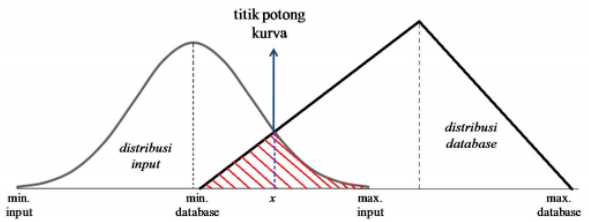
\includegraphics[width=0.5\linewidth]{images/screening/irisan}

\}

\textbackslash caption\{Daerah irisan dari distribusi \emph{input} dan distribusi \emph{database}\}\label{fig:unnamed-chunk-32}
\textbackslash end\{figure\}

Bagian kurva yang diarsir dengan warna merah pada gambar di atas memperlihatkan contoh daerah irisan dari dua kurva distribusi, yaitu kurva distribusi \emph{database} (segitiga) dan kurva distribusi \emph{input} (normal). Titik potong kurva (x) dicari dengan menggunakan metode numerik Newton-Raphson. Setelah titik potong kurva diperoleh, luas daerah irisan dihitung menggunakan aturan Simpson, \_seperti yang telah dijelaskan sebelumnya.

Berdasarkan penjelasan sebelumnya, maka terdapat empat kasus yang melibatkan pasangan distribusi database -- distribusi input, yaitu:
(1) Kasus pasangan distribusi segitiga -- distribusi segitiga
(2) Kasus pasangan distribusi segitiga -- distribusi normal
(3) Kasus pasangan distribusi segitiga -- distribusi uniform
(4) Kasus pasangan distribusi segitiga -- distribusi log normal.
Secara umum, pengembangan algoritma untuk setiap pasangan distribusi \emph{database} distribusi \emph{input} dibagi ke dalam enam tipe algoritma yang berlaku untuk enam kasus berikut:

\textbf{(1) Distribusi \emph{database} dan distribusi \emph{input} tidak berpotongan}\_
Distribusi \emph{database} dan distribusi \emph{input} tidak berpotongan jika interval distribusi \emph{input} berada di luar interval distribusi \emph{database}. Gambar di bawah memperlihatkan contoh kasus ini untuk pasangan distribusi \emph{database} segitiga distribusi \emph{input} normal. Karena kedua kurva distribusi tidak berpotongan, maka tidak terdapat daerah irisan antara dua distribusi ini, sehingga probabilitas kecocokan distribusi input terhadap distribusi database adalah nol.
\textbackslash begin\{figure\}

\{\centering 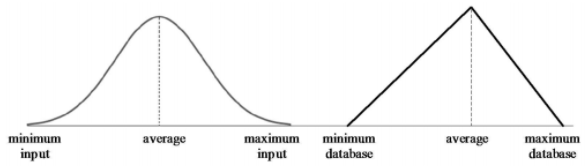
\includegraphics[width=0.5\linewidth]{images/screening/tidak_berpotongan}

\}

\textbackslash caption\{Distribusi \emph{input} dan distribusi \emph{database} tidak berpotongan\}\label{fig:unnamed-chunk-33}
\textbackslash end\{figure\}

~

\textbf{(2) Distribusi \emph{database} dan distribusi \emph{input} identik}
Hal ini terjadi jika distribusi \emph{database} dan distribusi \emph{input} memiliki bentuk distribusi yang sama dengan parameter-parameter nilai minimum, nilai maksimum, nilai \emph{mean}, dan nilai standard deviasi yang sama. Dengan kata lain, distribusi \emph{database} dan distribusi \emph{input} adalah dua distribusi identik. Karena dua distribusi identik, maka daerah irisan antara kedua distribusi ini meliputi seluruh daerah di bawah kurva kedua distribusi, sehingga probabilitas kecocokan distribusi \emph{input} terhadap distribusi \emph{database} adalah 100\%.
\textbackslash begin\{figure\}

\{\centering 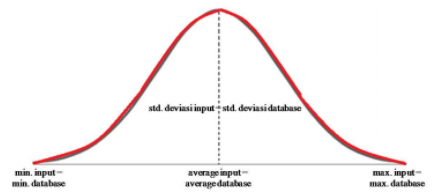
\includegraphics[width=0.5\linewidth]{images/screening/distribusi_identik}

\}

\textbackslash caption\{Distribusi \emph{input} dan distribusi \emph{database} merupakan distribusi identik\}\label{fig:unnamed-chunk-34}
\textbackslash end\{figure\}

~

\textbf{(3) Distribusi \emph{input} beririsan dengan distribusi \emph{database} di sisi kiri distribusi \emph{database}}
Untuk kasus ini, terdapat satu titik potong antara kurva distribusi \emph{database} dan kurva distribusi \emph{input.} Gambar di bawah memperlihatkan contoh untuk kasus ini.
\textbackslash begin\{figure\}

\{\centering 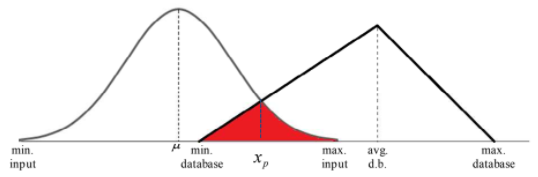
\includegraphics[width=0.5\linewidth]{images/screening/irisan1}

\}

\textbackslash caption\{Daerah irisan berada di sisi kiri kurva distribusi \emph{database}\}\label{fig:unnamed-chunk-35}
\textbackslash end\{figure\}

Pengembangan algoritma untuk kasus ini adalah sebagai berikut. Pertama, titik potong kurva dicari dengan menggunakan metode Newton. Fungsi yang digunakan dalam iterasi Newton adalah selisih antara kedua \emph{density function} dari distribusi \emph{database} dan distribusi \emph{input.} Jika distribusi \emph{database} memiliki \emph{density function f(x)} dan distribusi \emph{input} memiliki \emph{density function g(x)}, maka fungsi \emph{h(x) = f(x) − g(x)} menyatakan selisih dari fungsi distribusi \emph{database} dan fungsi distribusi \emph{input.}

Titik potong antara kedua kurva adalah suatu titik \emph{x} pada kurva dimana nilai fungsi \emph{h(x)} adalah nol. Nilai \emph{h(x)} nol adalah solusi eksak, sedangkan metode Newton adalah metode mencari solusi secara numerik. Oleh karena itu, dibutuhkan penyesuaian terhadap solusi numerik. Untuk solusi numerik, titik potong kurva dinyatakan oleh suatu titik \emph{x} pada kurva dimana nilai fungsi \emph{h(x)} sangat dekat dengan nol dengan tingkat kesalahan \emph{E}. Tingkat kesalahan \emph{E} yang digunakan pada algoritma adalah 10\textsuperscript{-7}. Sehingga, solusi titik potong x secara numerik adalah nilai dimana titik perulangan x\textsubscript{n+1} memenuhi \textbar{}\emph{x\textsubscript{n+1}} − \emph{x\textsubscript{n}}\textbar{} ≤ \emph{E}.

Setelah titik potong kurva diperoleh, langkah selanjutnya adalah menghitung luas daerah irisan antara dua kurva distribusi. Luas daerah irisan ini diperlihatkan di gambar dengan arsiran merah. Luas daerah irisan menyatakan probabilitas kecocokan ditribusi \emph{input} terhadap distribusi \emph{database}. Secara umum, untuk daerah irisan berada di sisi kiri kurva distribusi \emph{database}, luas daerah dihitung dengan cara berikut. \[Luas\ Daerah\ arsiran\ = \int_{min.db}^{x_p}g(x)dx\ +\ \int_{x_p}^{max.input}f(x)dx...(27) \]
Dimana \(\int_{min.db}^{x_p}g(x)dx\) dan \(\int_{x_p}^{max.input}f(x)dx\) dihitung menggunakan aturan Simpson.

~

\textbf{(4) Distribusi \emph{input} beririsan dengan distribusi \emph{database} di sisi kanan distribusi \emph{database}}
Kasus ini masih melibatkan satu titik potong. Contoh kasus ini diperlihatkan pada hambar berikut.
\textbackslash begin\{figure\}

\{\centering 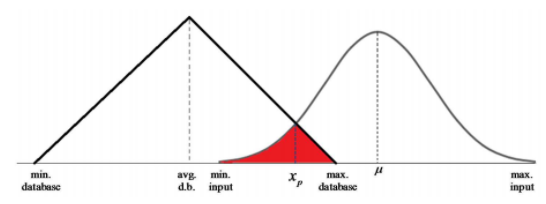
\includegraphics[width=0.5\linewidth]{images/screening/irisan2}

\}

\textbackslash caption\{Daerah irisan berada di sisi kanan kurva distribusi \emph{database}\}\label{fig:unnamed-chunk-36}
\textbackslash end\{figure\}

Langkah-langkah pengembangan algoritma untuk kasus ini sama seperti kasus (3) di atas, yaitu penentuan titik potong x\textsubscript{p} yang diikuti oleh perhitungan luas daerah arsiran untuk mengetahui probabilitas kecocokan distribusi \emph{input} terhadap distribusi \emph{database}. Secara umum, perhitungan luas daerah arsiran adalah: \[Luas\ daerah\ arsiran\ = \int_{min.input}^{x_p}g(x)dx\ +\ \int_{x_p}^{max.db}f(x)dx...(28) \]
Dimana \(\int_{min.input}^{x_p}g(x)dx\) dan \(\int_{x_p}^{max.db}f(x)dx\) dihitung menggunakan aturan Simpson.

~

\textbf{(5) Interval distribusi \emph{input} berada di dalam interval distribusi \emph{database}}
Berbeda dengan kasus (3) dan (4), kasus ini memiliki dua titik potong. Pada dasarnya, langkah-langkah pengembangan algoritma untuk dua titik potong sama seperti kasus satu titik potong, yaitu penentuan titik potong (dalam hal ini terdapat dua titik potong) kemudian menghitung luas daerah arsiran untuk mengetahui probabilitas kecocokan distribusi \emph{inpu}. terhadap distribusi \emph{database}.
\textbackslash begin\{figure\}

\{\centering 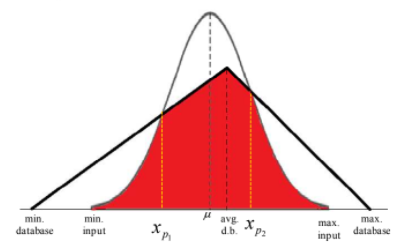
\includegraphics[width=0.5\linewidth]{images/screening/interval_dalam}

\}

\textbackslash caption\{Kasus interval distribusi \emph{input} berada di dalam distribusi \emph{database}\}\label{fig:unnamed-chunk-37}
\textbackslash end\{figure\}
Luas daerah arsiran dihitung menggunkn persamaan berikut. \[Luas\ Daerah\ arsiran\ = \int_{min.input}^{x_{p_1}}g(x)dx\ +\ \int_{x_{p_1}}^{avg.db}f_1(x)dx\ +\ \int_{avg.db}^{x_{p_2}}f_2(x)dx\ +\ \int_{x_{p_2}}^{max.input}g(x)dx...(29)\]
Masing-masing integral di atas dihitung menggunakan aturan Simpson.

~

\textbf{(6) Interval distribusi \emph{database} berada di dalam interval distribusi \emph{input}}
Sama seperti kasus (5), kasus ini melibatkan dua titik potong. Langkah-langkah pengembangan algoritma sama seperti kasus-kasus sebelumnya, yaitu penentuan titik potong yang dilanjutkan dengan perhitungan luas daerah arsiran untuk mengetahui probabilitas kecocokan distribusi \emph{input} terhadap distribusi \emph{database}.
\textbackslash begin\{figure\}

\{\centering 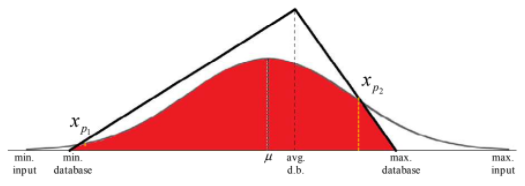
\includegraphics[width=0.5\linewidth]{images/screening/interval_dalam1}

\}

\textbackslash caption\{Kasus interval distribusi \emph{database} berada di dalam distribusi \emph{input}\}\label{fig:unnamed-chunk-38}
\textbackslash end\{figure\}
Luas daerah arsiran adalah: \[Luas\ daerah\ arsiran\ = \int_{min.input}^{x_{p_1}}f_1(x)dx\ +\ \int_{x_{p_1}}^{\mu}g(x)dx\ +\ \int_{\mu}^{x_{p_2}}g(x)dx\ +\ \int_{x_{p_2}}^{max.input}f_2(x)dx...(30)\]
Masing-masing integral di atas dihitung menggunakan aturan Simpson.

Masing-masing keenam kasus di atas berlaku untuk keempat pasangan distribusi \emph{database} -- distribusi \emph{input.} Langkah-langkah pengembangan algoritma adalah sama untuk setiap pasangan distribusi \emph{database} -- distribusi \emph{input.} Perbedaannya terletak pada fungsi \emph{g(x)} yang menyatakan \emph{density} \emph{function} dari distribusi \emph{input.} Karena terdapat empat pilihan distribusi input, maka terdapat empat pilihan fungsi \emph{g(x)} yang berbeda bersesuaian dengan tipe distribusi \emph{input} yang dipilih oleh \emph{user.} Secara umum, diagram alir algoritma untuk kasus input berupa distribusi diperlihatkan pada gambar berikut.

\textbackslash begin\{figure\}

\{\centering 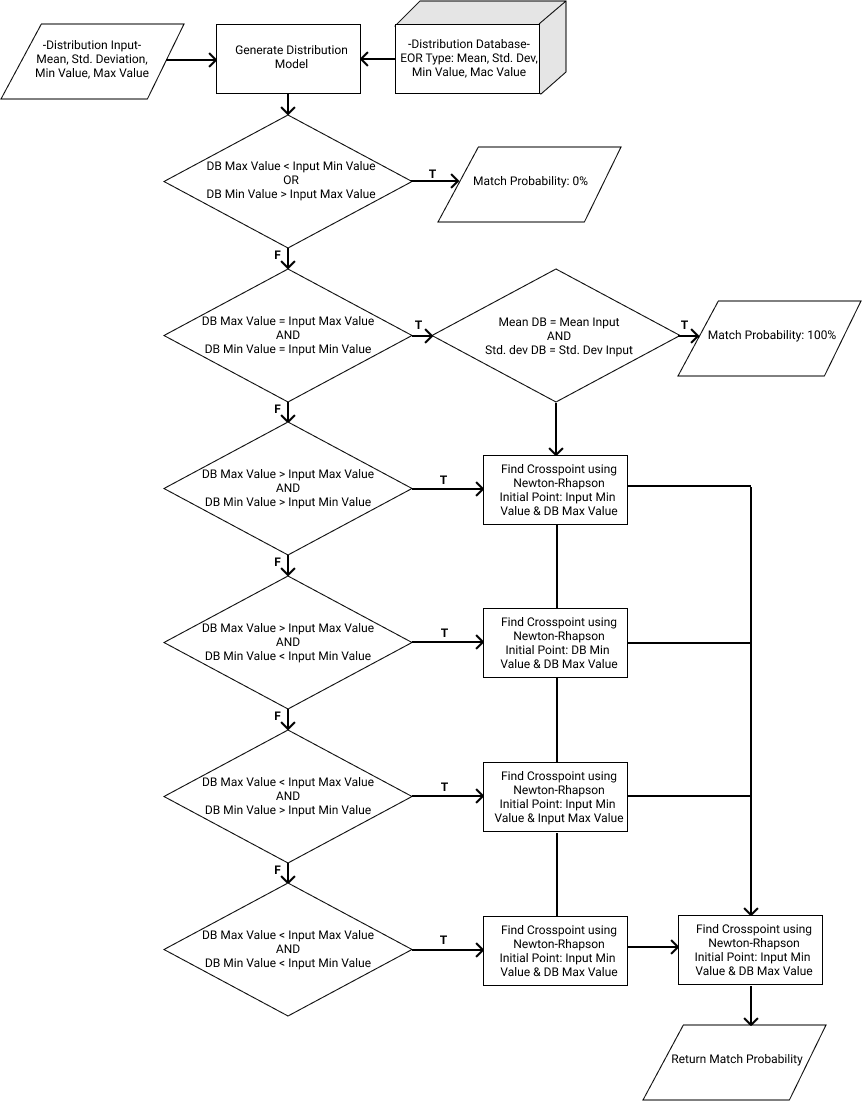
\includegraphics[width=0.75\linewidth]{images/screening/flowchart}

\}

\textbackslash caption\{Diagram alir algoritma EOR \emph{screening} untuk kasus distribusi\}\label{fig:unnamed-chunk-39}
\textbackslash end\{figure\}

\hypertarget{co2-prophet-predictive-model}{%
\chapter{\texorpdfstring{CO\textsubscript{2} Prophet Predictive Model}{CO2 Prophet Predictive Model}}\label{co2-prophet-predictive-model}}

\hypertarget{pendahuluan}{%
\section{Pendahuluan}\label{pendahuluan}}

\textbf{CO\textsubscript{2} Prophet} merupakan perangkat lunak yang dibangun oleh \textbf{U.S. Department of Energy (DOE)} yang dapat digunakan untuk memprediksi performa CO2 \emph{flooding}. Perangkat lunak ini memiliki keunggulan dibandingkan dengan CO2 Miscible Predictive Model (CO2PM), yang juga dibangun oleh U.S. DOE.

Berbeda dengan CO2PM yang hanya memberikan satu pilihan pola injeksi (yaitu 5-spot), CO\textsubscript{2} Prophet memberikan opsi kepada \emph{user} untuk memilih antara enam pola injeksi. Pilihan pola injeksi yang tersedia diantaranya adalah 5-\emph{spot}, West Texas 7-\emph{spot}, \emph{Inverted} 9-\emph{spot}, \emph{Line Drive}, 4-\emph{spot}, dan \emph{Isolated} 2-\emph{spot.} Gambar berikut memperlihatkan pilihan pola injeksi yang tersedia bagi \emph{user}.

\begin{figure}

{\centering 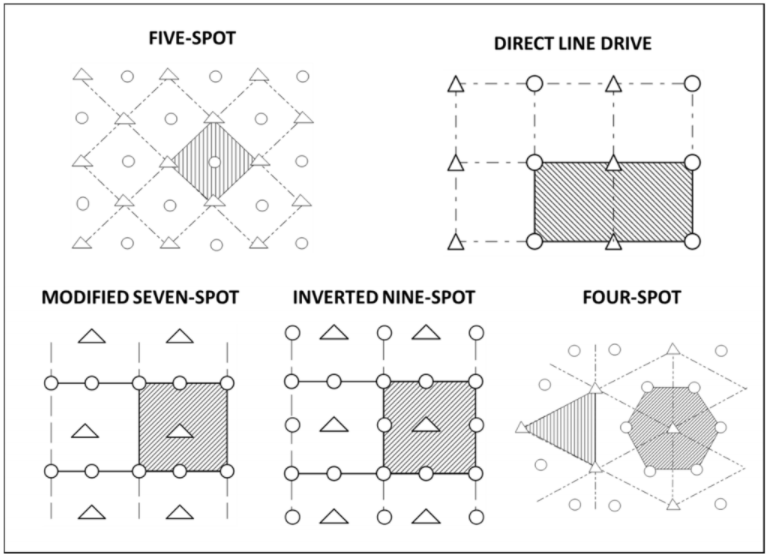
\includegraphics[width=0.5\linewidth]{images/co2prophet/patternCO2} 

}

\caption{Beberapa pilihan pola injeksi dalam CO~2~ Prophet}\label{fig:unnamed-chunk-41}
\end{figure}

~

Selain untuk memprediksi performa \emph{miscible} CO\textsubscript{2} \emph{flooding}, CO\textsubscript{2} Prophet juga dapat digunakan untuk memprediksi performa \emph{waterflood}, \emph{miscible} CO\textsubscript{2} \emph{WAG}, dan \emph{immiscible} CO\textsubscript{2} \emph{flood.}

~

\hypertarget{asumsi-yang-digunakan-dalam-model}{%
\section{Asumsi yang Digunakan Dalam Model}\label{asumsi-yang-digunakan-dalam-model}}

Beberapa asumsi yang digunakan dalam CO\textsubscript{2} Prophet diantaranya adalah:

\begin{enumerate}
\def\labelenumi{\arabic{enumi}.}
\tightlist
\item
  Terdapat tiga fasa fluida yang disertakan dalam model, yaitu fasa minyak, fasa air, dan fasa \emph{solvent.}
\item
  User dapat memilih hingga 10 \emph{layer} untuk digunakan dalam perhitungan. Nilai \emph{default} untuk jumlah \emph{layer} adalah 5 \emph{layer.}
\item
  Efek gravitasi diabaikan.
\item
  Beberapa parameter reservoir dan fluida yang berperan penting dalam model diantaranya adalah koefisien permeabilitas Dykstra-Parsons, viskositas minyak, viskositas air, temperatur
  reservoir, tekanan rata-rata reservoir, dan \emph{minimum miscibility pressure} (MMP).
\end{enumerate}

\hypertarget{parameter-parameter-penting-yang-digunakan-dalam-model}{%
\section{Parameter-Parameter Penting yang Digunakan Dalam Model}\label{parameter-parameter-penting-yang-digunakan-dalam-model}}

\hypertarget{koefisien-permeabilitas-dykstra-parsons}{%
\subsection{Koefisien Permeabilitas Dykstra-Parsons}\label{koefisien-permeabilitas-dykstra-parsons}}

Koefisien permeabilitas Dykstra-Parsons (V\textsubscript{\emph{dp}}) menyatakan besarnya keheterogenan permeabilitas reservoir secara vertikal. Nilai V\textsubscript{\emph{dp}} menentukan besarnya \emph{injectivity} fluida di setiap lapisan reservoir. Nilai \emph{default} yang digunakan adalah 0.7.

\hypertarget{temperatur-reservoir}{%
\subsection{Temperatur Reservoir}\label{temperatur-reservoir}}

Dalam model, temperatur reservoir digunakan untuk menghitung viskositas CO\textsubscript{2} di dalam reservoir. Nilai \emph{default} yang digunakan adalah 100\(^\circ\)F.

\hypertarget{tekanan-rata-rata-reservoir-average-reservoir-pressure}{%
\subsection{\texorpdfstring{Tekanan Rata-Rata Reservoir (\emph{Average Reservoir Pressure})}{Tekanan Rata-Rata Reservoir (Average Reservoir Pressure)}}\label{tekanan-rata-rata-reservoir-average-reservoir-pressure}}

Nilai tekanan rata-rata reservoir menentukan kondisi aliran di reservoir. Kondisi aliran dapat berupa \emph{completely miscible flood}, \emph{partially miscible flood}, atau \emph{totally miscible flood}. Nilai \emph{default} yang digunakan dalam model adalah 2000 psia.

\hypertarget{minimum-miscibility-pressure-mmp}{%
\subsection{\texorpdfstring{\emph{Minimum Miscibility Pressure (MMP)}}{Minimum Miscibility Pressure (MMP)}}\label{minimum-miscibility-pressure-mmp}}

Sama seperti nilai tekanan rata-rata reservoir, nilai MMP menentukan kondisi aliran yang akan terjadi di reservoir. Jika \emph{user} menginginkan kondisi \emph{completely miscible} CO\textsubscript{2}, maka nilai MMP harus berada di bawah nilai tekanan rata-rata reservoir. Nilai default MMP yang digunakan dalam model adalah 1200 psia.

\hypertarget{viskositas-minyak-mu_o}{%
\subsection{\texorpdfstring{Viskositas Minyak (\(\mu_o\))}{Viskositas Minyak (\textbackslash mu\_o)}}\label{viskositas-minyak-mu_o}}

Dalam model, viskositas minyak digunakan untuk melakukan perhitungan mobilitas fluida. Nilai \emph{default} \(\mu_o\) yang digunakan dalam model adalah 2 cp.

\hypertarget{viskositas-air-mu_w}{%
\subsection{\texorpdfstring{Viskositas Air (\(\mu_w\))}{Viskositas Air (\textbackslash mu\_w)}}\label{viskositas-air-mu_w}}

Dalam model, viskositas minyak digunakan untuk melakukan perhitungan mobilitas fluida. Nilai \emph{default} \(\mu_w\) yang digunakan dalam model adalah 0.8 cp.

\hypertarget{faktor-volume-formasi-minyak-bo}{%
\subsection{\texorpdfstring{Faktor Volume Formasi Minyak (B\textsubscript{\emph{o}})}{Faktor Volume Formasi Minyak (Bo)}}\label{faktor-volume-formasi-minyak-bo}}

Faktor volume formasi minyak menyatakan perbandingan antara volume fluida di reservoir dengan volume fluida di permukaan. Nilai default yang digunakan dalam model adalah 1.4 bbl/STB.

\hypertarget{solution-gas-oil-ratio-rs}{%
\subsection{\texorpdfstring{\emph{Solution Gas-Oil Ratio} (R\textsubscript{\emph{s}})}{Solution Gas-Oil Ratio (Rs)}}\label{solution-gas-oil-ratio-rs}}

Nilai kelarutan gas digunakan untuk menghitung jumlah gas hidrokarbon yang terproduksikan. Nilai \emph{defaut} yang digunakan dalam model adalah 500 scf/STB.

\hypertarget{permeabilitas-relatif-kr}{%
\subsection{\texorpdfstring{Permeabilitas Relatif (k\textsubscript{\emph{r}})}{Permeabilitas Relatif (kr)}}\label{permeabilitas-relatif-kr}}

Dalam model, nilai permeabilitas relatif air (k\textsubscript{\emph{rw}}), permeabilitas relatif minyak (k\textsubscript{\emph{ro}}), permeabilitas relatif gas (k\textsubscript{\emph{rg}}), dan permeabilitas relatif solvent (k\textsubscript{\emph{rs}}) dihitung menggunakan persamaan-persamaan berikut:
\[k_{rw}\ = k_{rw}@S_{or} \left( \frac{S_w-S_{wirr}}{1-S_{wirr}-S_{orw}} \right)^{expw} \]
\[k_{ro}\ (oil\ -\ water) = k_{ro}@S_{wc} \left( \frac{1-S_w-S_{orw}}{1-S_{wc}-S_{orw}} \right)^{expow} \]
\[k_{ro}\ (gas\ -\ oil) = k_{ro}@S_{wc} \left( \frac{1-S_{wc}-S_{org}-S_g}{1-S_{wc}-S_{org}} \right)^{expog} \]
\[k_{rg}\ = k_{rg}@S_{wc} \left( \frac{S_g-S_{gr}}{1-S_{wc}-S_{gr}} \right)^{expg} \]
\[k_{rs}\ = k_{rs}@S_{wc} \left( \frac{S_g-S_{gr}}{1-S_{wirr}-S_{sr}-S_{orm}} \right)^{exps} \]
Dimana:
\emph{S\textsubscript{wirr}} = \emph{irreducible water saturation (default = 0.2)}
\emph{S\textsubscript{orw}} = \emph{residual oil to waterflood (default = 0.37)}
\emph{S\textsubscript{wc}} = \emph{connate water saturation (default = 0.2)}
\emph{S\textsubscript{gr}} = \emph{residual gas saturation (default = 0.37)}
\emph{S\textsubscript{sr}} = \emph{residual solvent saturation (default = 0.37)}
\emph{S\textsubscript{orm}} = \emph{residual oil saturation to solvent (default = 0.001)}
expw = \emph{water equation exponent (default = 2)}
expo = \emph{oil equation exponent (default = 2)}
expw = \emph{gas equation exponent (default = 2)}
expo = \emph{solvent equation exponent (default = 2)}

\hypertarget{waterco2-injection-ratio}{%
\subsection{\texorpdfstring{\emph{Water/CO\textsubscript{2} Injection Ratio}}{Water/CO2 Injection Ratio}}\label{waterco2-injection-ratio}}

\textbf{\emph{Water/CO\textsubscript{2} Injection Ratio}} merupakan parameter yang menyatakan periode injeksi air dan CO\textsubscript{2} dalam injeksi WAG. Parameter ini terkait dengan \textbf{\emph{WAG ratio}}, seperti diperlihatkan pada tabel di bawah berikut ini.

\begin{longtable}[]{@{}cc@{}}
\caption{{ Tabel 1.1: Hubungan antara WAG \emph{ratio} dan \emph{water/CO\textsubscript{2} injection ratio} }}\tabularnewline
\toprule
WAG Ratio & Water/CO\textsubscript{2} Injection Ratio\tabularnewline
\midrule
\endfirsthead
\toprule
WAG Ratio & Water/CO\textsubscript{2} Injection Ratio\tabularnewline
\midrule
\endhead
2 to 1 & 2\tabularnewline
1 to 1 & 1\tabularnewline
1 to 2 & 0.5\tabularnewline
1 to 3 & 0.33\tabularnewline
\bottomrule
\end{longtable}

\emph{Water/CO\textsubscript{2} injection ratio} daoat ditentukan berdasarkan \emph{time basis} atau \emph{volume basis}. Jika \emph{user} memilih \emph{time basis} dan nilai \emph{water/CO\textsubscript{2} injection ratio} adalah 2, maka 67\% dari total periode injeksi adalah injeksi air, dan 33\% dari total periode injeksi adalah injeksi CO\textsubscript{2}. Jika \emph{user} memilih \emph{volume basis} dan nilai \emph{water/injection ratio} adalah 2, maka 67\% dari total volume injeksi fluida adalah air, dan 33\% dari total volume injeksi fluida adalah CO\textsubscript{2}.

\hypertarget{mixing-parameter-omega}{%
\subsection{\texorpdfstring{\emph{Mixing Parameter (\(\omega\))}}{Mixing Parameter (\textbackslash omega)}}\label{mixing-parameter-omega}}

\emph{Mixing parameter} merupakan parameter yang digunakan untuk menggambarkan keadaan \emph{miscibility} di dalam model. Parameter ini berperan dalam mengatur viskositas efektif untuk fasa \emph{solvent} dan minyak. Jika , bernilai 0, maka tidak terjadi pencampuran dan fasa \emph{solvent} dan minyak memiliki nilai viskositas yang berbeda, masing-masing sesuai dengan nilai \emph{immiscible}-nya. Jika \(\omega\), bernilai 1, maka terjadi complete mixing dimana fasa minyak dan \emph{solvent} akan memiliki viskositas yang sama. Nilai default yang digunakan untuk, adalah 0.666.

Viskositas efektif untuk fasa minyak dan \emph{solvent} masing-masing dinyatakan oleh persamaan berikut:
\[Viskositas\ efektif\ solvent\ = \mu_{se} = (1-\alpha)\mu_s\ + \alpha\mu_{sm} \]
\[Viskositas\ efektif\ minyak\ = \mu_{oe} = (1-\alpha)\mu_o\ + \alpha\mu_{pm} \]

~

Untuk kondisi \emph{partially miscible}, yaitu P\textsubscript{\emph{res}} \textless{} \emph{MMP} dan P\textsubscript{\emph{res}} \textgreater{} 0.75\_MMP\_, maka \(\alpha\) dinyatakan oleh:
\[\alpha = \frac{P_{res}-0.75MMP}{0.25MMP}\]

~

Untuk kondisi \emph{completely miscible}, yaitu P\textsubscript{\emph{res}} \textgreater{} \emph{MMP}, maka \(\alpha\) dinyatakan oleh:
\[\alpha = 1\]
\[\mu_{sm} = \mu_s^{1-\omega}\mu_m^\omega\]
\[\mu_{om} = \mu_o^{1-\omega}\mu_m^\omega\]
\[\frac{1}{\mu_m^{0.25}} = \frac{1}{1-S_w} \left(\frac{S_o}{\mu_o^{0.25}} + \frac{S_g}{\mu_s^{0.25}} \right)\]

Dimana:
\emph{\(\mu_s\) = solvent viscosity}
\emph{\(\mu_o\) = oil viscosity}
\emph{\(\mu_m\) = mixed viscosity}
\emph{\(\mu_{sm}\) = mixed solvent viscosity}
\emph{\(\mu_{om}\) = mixed oil viscosity}

\hypertarget{tiga-kondisi-aliran-fluida}{%
\section{Tiga Kondisi Aliran Fluida}\label{tiga-kondisi-aliran-fluida}}

Proses \emph{flooding} dapat terjadi dalam tiga kondisi, yaitu kondisi \emph{immiscible flow}, \emph{miscible flow}, dan \emph{partially miscible flow}.

\hypertarget{immiscible-flow}{%
\subsection{\texorpdfstring{\emph{Immiscible Flow}}{Immiscible Flow}}\label{immiscible-flow}}

Pada kondisi aliran \emph{immiscible}, permeabilitas relatif solvent merupakan fungsi dari saturasi \emph{solvent} saja. Pada kondisi ini, permeabilitas relatif minyak (\emph{k}\textsubscript{\emph{ro}}) dinyatakan oleh:

\[k_{ro} = \frac{1}{k_{row}}(A-k_{rg}-k_{rw})\]
\[A = \left( \frac{k_{row}}{k_{ro}@S_{wc}}+k_{rw}\right)\left( \frac{k_{rog}}{k_{ro}@S_{wc}}+k_{rg}\right) \]

\hypertarget{miscible-flow}{%
\subsection{\texorpdfstring{\emph{Miscible Flow}}{Miscible Flow}}\label{miscible-flow}}

Pada kondisi aliran \emph{miscible}, permeabilitas relatif fasa \emph{miscible} (\emph{k}\textsubscript{\emph{rm}}) dihitung dengan persamaan berikut.
\[k_{rm} = \frac{S_o-S_{orm}}{1-S_w-S_{orm}}(k_{row})\ +\ \frac{S_g}{1-S_w-S_{orm}}(k_{rs}) \]

\hypertarget{partially-miscible-flow}{%
\subsection{\texorpdfstring{\emph{Partially Miscible Flow}}{Partially Miscible Flow}}\label{partially-miscible-flow}}

Kondisi \emph{partially miscible} terjadi saat P\textsubscript{\emph{res}} \textless{} \emph{MMP} dan P\textsubscript{\emph{res}} \textgreater{} 0.75\emph{MMP}. Pada kondisi ini, permeabilitas efektif minyak dan \emph{solvent} dinyatakan oleh persamaan berikut.
\[k_{roeff} = (1-\alpha)k_{ro}\ +\ \alpha \left( \frac{S_o-S_{orm}}{1-S_w-S_{orm}} \right)\]
\[k_{rseff} = (1-\alpha)k_{rg}\ +\ \alpha \left( \frac{S_g}{1-S_w-S_{orm}}(k_{rs} \right)\]

dimana:
\[\alpha = \frac{P_{res}-0.75MMP}{0.25MMP}\]

\hypertarget{hasil-perhitungan-dan-tampilan-perangkat-lunak}{%
\section{Hasil Perhitungan dan Tampilan Perangkat Lunak}\label{hasil-perhitungan-dan-tampilan-perangkat-lunak}}

Hasil perhitungan CO\textsubscript{2} Prophet memberikan informasi mengenai estimasi dari beberapa parameter performa produksi, diantaranya laju produksi minyak, laju produksi air, laju produksi CO\textsubscript{2}, dan lain sebagainya.

Berikut merupakan tampilan \emph{screenshot} dari \emph{output} yang dihasilkan oleh CO\textsubscript{2} Prophet.

\begin{figure}

{\centering 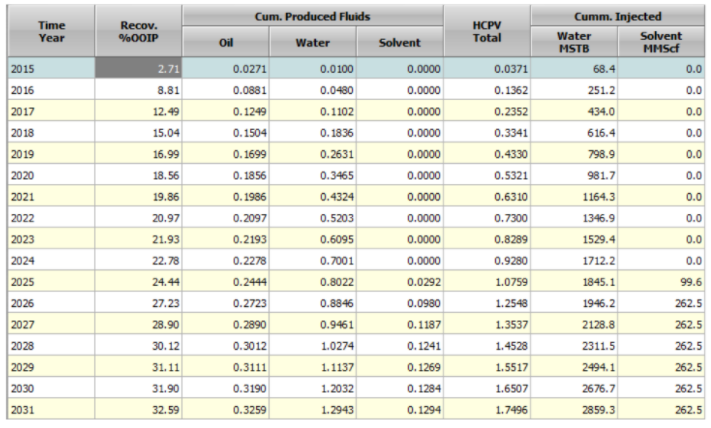
\includegraphics[width=0.5\linewidth]{images/co2prophet/prediksiprophet} 

}

\caption{Hasil prediksi performa dari CO~2~ Prophet}\label{fig:unnamed-chunk-42}
\end{figure}

~

\begin{figure}

{\centering 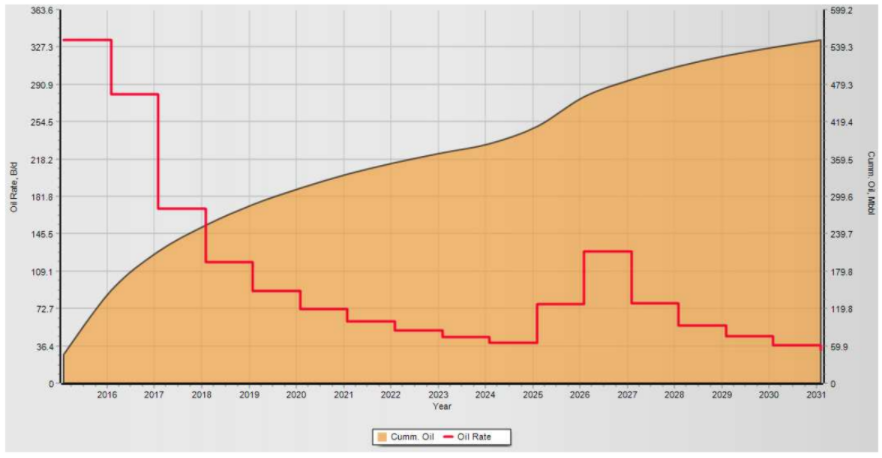
\includegraphics[width=0.5\linewidth]{images/co2prophet/produksiminyakprophet} 

}

\caption{Grafik laju produksi minyak hasil perhitungan CO~2~ Prophet}\label{fig:unnamed-chunk-43}
\end{figure}

~

\begin{figure}

{\centering 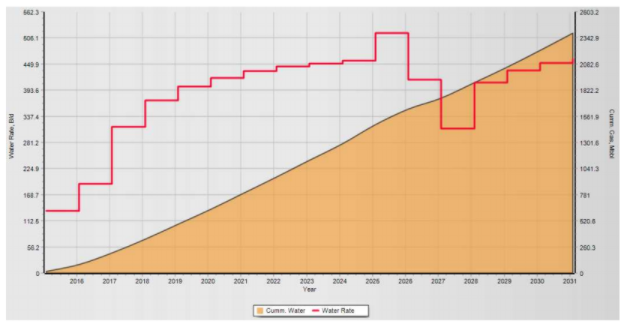
\includegraphics[width=0.5\linewidth]{images/co2prophet/produksiairprophet} 

}

\caption{Grafik laju produksi air hasil perhitungan CO~2~ Prophet}\label{fig:unnamed-chunk-44}
\end{figure}

~

\textbackslash begin\{figure\}

\{\centering 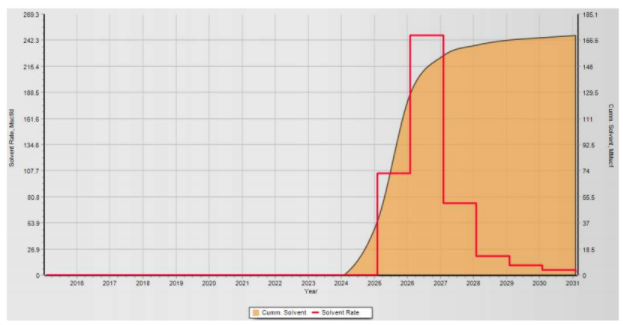
\includegraphics[width=0.5\linewidth]{images/co2prophet/produksisolventprophet}

\}

\textbackslash caption\{Grafik laju produksi \emph{solvent} hasil perhitungan CO\textsubscript{2} Prophet\}\label{fig:unnamed-chunk-45}
\textbackslash end\{figure\}

~

\hypertarget{waterflood-predictive-model}{%
\chapter{Waterflood Predictive Model}\label{waterflood-predictive-model}}

\hypertarget{pendahuluan-1}{%
\section{Pendahuluan}\label{pendahuluan-1}}

\textbf{\emph{Waterflooding}} adalah istilah yang digunakan untuk menggambarkan proses injeksi air ke dalam reservoir dengan tujuan untuk menambah tingkat perolehan minyak. \emph{Waterflood predictive model} merupakan suatu model yang dapat memprediksi performa reservoir di bawah proses \emph{waterflood}.

Analisis performa \emph{waterflood} membutuhkan informasi mengenai profil saturasi air di reservoi selama periode injeksi air dilakukan. Teori \textbf{\emph{frontal displacement}} dari Buckley dan Leverett merupakan teori yang membahas mengenai cara menentukan profil saturasi air di reservoir selama proses \emph{secondary} atau \emph{tertiary recovery}. Teori ini tidak hanya berlaku untuk prediksi performa reservoir di bawah proses \emph{waterflooding}, tetapi juga berlaku umum untuk seluruh proses \emph{secondary} dan \emph{tertiary flooding}. Pemahaman mengenai teori \emph{frontal displacement}, yang terdiri dari teori \textbf{fractional flow} dan teori \textbf{frontal advance}, sangat penting untuk memprediksi performa reservoir di bawah proses \emph{secondary} maupun \emph{tertiary flooding}. Berikut akan diberikan pnjelasan mengenai teori \emph{frontal displacement}.

\hypertarget{teori-frontal-displacement-untuk-waterflooding}{%
\section{\texorpdfstring{Teori \emph{Frontal Displacement} Untuk \emph{Waterflooding}}{Teori Frontal Displacement Untuk Waterflooding}}\label{teori-frontal-displacement-untuk-waterflooding}}

\hypertarget{teori-fractional-flow-untuk-waterflooding}{%
\subsection{\texorpdfstring{Teori \emph{Fractional Flow} Untuk \emph{Waterflooding}}{Teori Fractional Flow Untuk Waterflooding}}\label{teori-fractional-flow-untuk-waterflooding}}

Teori \emph{fractional flow} merupakan teori yang membahas mengenai fraksi aliran suatu fasa fluida dalam total aliran yang terdiri atas sejumlah fasa fluida. Melalui teori \emph{fractional flow}, nilai dari fraksi aliran air sebagai fungsi dari saturasi air di reservoir dapat diketahui. Berikut akan dijelaskan mengenai penurunan persamaan \emph{fractional flow}.

Tinjau dua fasa fluida yang mengalir bersamaan di reservoir, yaitu fasa air (\emph{water}) dan fasa minyak (\emph{oil}). Persamaan Darcy (dalam bentuk kecepatan alir Darcy) untuk masing-masing fasaini dinyatakan sebagai berikut.
\[u_o = -\frac{k_o}{\mu_o} \left[ \frac{\partial P_o}{\partial x}+ \rho_o\ g\ \sin \alpha \right]\]
\[u_w = -\frac{k_w}{\mu_w} \left[ \frac{\partial P_w}{\partial x}+\rho_w\ g\ \sin \alpha \right] ... (1)\]Pada persamaan (1) di atas, \emph{k\textsubscript{i}} menyatakan permeabilitas efektif dari masing-masing fasa. Selanjutnya, dari definisi kecepatan Darcy,
\[u = \frac{q}{A}...(2)\]
Maka substitusi persamaan (2) ke persamaan (1) akan memberikan persamaan berikut.
\[q_o = \frac{-k_o A}{\mu_o} \left[ \frac{\partial P_o}{\partial x}+ \rho_o\ g\ \sin \alpha \right] \]
\[q_w = \frac{-k_w A}{\mu_w} \left[ \frac{\partial P_w}{\partial x}+ \rho_w\ g\ \sin \alpha \right]...(3) \]
Fraksi aliran air (\emph{fractional flow of water - f\textsubscript{w}}) dari total aliran didefinisikan sebagai laju alir fasa air dibagi dengan laju alir total,
\[f_w = \frac{q_w}{q_t} = \frac{q_w}{q_w+q_o}...(4)\]
Dari persamaan (4), diperoleh dua persamaan berikut:
\[q_w = f_w\ q_t\]
\[q_o = (1-f_w)\ q_t\]
Substitusi persamaan (5) ke persamaan (3), maka persamaan aliran untuk fasa minyak dan fasa air menjadi:
\[(1-f_w)\ q_t = -\frac{k_o A}{\mu_o} \left[ \frac{\partial P_o}{\partial x}+ \rho_o\ g\ \sin \alpha \right]\]
\[f_w\ q_t = -\frac{k_w A}{\mu_w} \left[ \frac{\partial P_w}{\partial x}+ \rho_w\ g\ \sin \alpha \right]\]
Persamaan di atas dapat pula dituliskan sebagai:
\[-(1-f_w) \frac{q_t}{A} \frac{\mu_o}{k_o} = \frac{\partial P_o}{\partial x}+ \rho_o\ g\ \sin \alpha \]
\[-f_w \frac{q_t}{A} \frac{\mu_w}{k_w} = \frac{\partial P_w}{\partial x}+ \rho_o\ g\ \sin \alpha...(6) \]
Selanjutnya, dari definisi tekanan kapiler, \emph{P\textsubscript{c} = P\textsubscript{o} - P\textsubscript{w}}, diperoleh
\[\frac{\partial P_c}{\partial x} = \frac{\partial P_o}{\partial x} - \frac{\partial P_w}{\partial x}...(7)\]
Selisihkan persamaan aliran fasa minyak dan fasa air dari persamaan (6), kemudian lakukan substitusi persamaan (7) ke persamaan (6), diperoleh:
\[\frac{q_t f_w}{A} \left( \frac{\mu_o}{k_o} +\frac{\mu_w}{k_w} \right) = \frac{\partial P_c}{\partial x} + (\rho_o - \rho_g)\ g\ sin\ \alpha\ + \frac{q_t}{A} \frac{\mu_o}{k_o} \]
\[\frac{q_t f_w}{A} = \frac{\frac{\partial P_c}{\partial x} + (\rho_o - \rho_g)\ g\ sin\ \alpha\ + \frac{q_t}{A} \frac{\mu_o}{k_o}}{\left( \frac{\mu_o}{k_o} +\frac{\mu_w}{k_w} \right)}\]
\[f_w = \frac{1+\frac{k_o}{\mu_o}\frac{A}{q_t} \left( \frac{\partial P_c}{\partial x} + (\rho_o - \rho_g)\ g\ sin\ \alpha\ \right)}{1+\frac{k_o}{k_w}\frac{\mu_w}{\mu_o}}...(8)\]
Persamaan (8) merupakan persamaan \emph{fractional flow} untuk fasa air. Jika faktor tekanan kapiler dapat diabaikan, dan reservoir berada pada bidang horizontal ( = 0), maka bentuk persamaan \emph{fractional flow of water} dapat menjadi lebih sederhana, yaitu:
\[f_w = \frac{1}{1+\frac{k_o}{k_w}\frac{\mu_w}{\mu_o}}...(9)\]
Persamaan (9) dapat pula dinyatakan dalam bentuk permeabilitas relatif, yaitu:
\[f_w = \frac{1}{1+\frac{k_{ro}}{k_{rw}}\frac{\mu_w}{\mu_o}}...(10)\]
Analisis lebih lanjut perlu dilakukan terhadap persamaan fraksi aliran air sehingga informasi mengenai nilai fraksi aliran air (\emph{f\textsubscript{w}}) sebagai fungsi dari saturasi air (\emph{S\textsubscript{w}}) di reservoir dapat diperoleh. Plot fraksi aliran air (\emph{f\textsubscript{w}}) terhadap saturasi air (\emph{S\textsubscript{w}}) memiliki bentuk kurva seperti pada gambar berikut.

\begin{figure}

{\centering 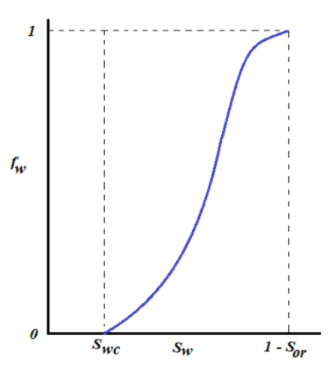
\includegraphics[width=0.5\linewidth]{images/waterflood/fraksiair} 

}

\caption{Kurva fraksi aliran air sebagai fungsi dari saturasi air}\label{fig:unnamed-chunk-47}
\end{figure}

~

Untuk menyusun kurva \emph{f\textsubscript{w}} versus \emph{S\textsubscript{w}} seperti di atas, perlu diketahui pernyataan \emph{f\textsubscript{w}} sebagai fungsi dari \emph{S\textsubscript{w}}, \({f_w = f_w(S_w)}\). Approksimasi pernyataan \({f_w = f_w(S_w)}\) dapat diperoleh melalui analisis kurva rasio permeabilitas relatif terhadap .. Beberapa persamaan berikut memberikan approksimasi nilai fraksi aliran air sebagai fungsi dari saturasi air.
\[\frac{k_{ro}}{k_{rw}} = ae^{bS_w} ...(11)\]
\[f_w = \frac{1}{1+ \left( \frac{\mu_w}{\mu_o} \right)ae^{bS_w}}...(12)\]
\[\left( \frac{\partial f_w}{\partial S_w} \right)_{S_w} = \frac{- \left( \frac{\mu_w}{\mu_o} \right)abe^{bS_w}}{\left[ 1+ \left( \frac{\mu_w}{\mu_o} \right)ae^{bS_w} \right]^2}...(13)\]
Dari kurva rasio permeabilitas relatif (k\textsubscript{ro}/k\textsubscript{rw}) terhadap saturasi air (\emph{S\textsubscript{w}}), nilai koefisien \emph{a} dan \emph{b} pada persamaan (11) dapat diketahui. Setelah koefisien \emph{a} dan \emph{b} diketahui, maka persamaan (12) dapat digunakan sebagai approksimasi untuk mengetahui nilai \emph{f\textsubscript{w}} sebagai fungsi \emph{S\textsubscript{w}}. Turunan dari \emph{f\textsubscript{w}} terhadap \emph{S\textsubscript{w}}, yaitu (\(\frac{\partial f_w}{\partial S_w}\)), merupakan parameter yang sangat penting dalam penentuan profil saturasi air. Penjelasan mengenai parameter (\(\frac{\partial f_w}{\partial S_w}\)) akan diberikan kemudian pada subbab tentang teori \emph{frontal advance}.

Kembali ke pembahasan mengenai persamaan \emph{fractional flow}, seperti dijelaskan di awal subbab, persamaan \emph{fractional flow} adalah persamaan yang memberikan nilai fraksi aliran air sebagai fungsi dari saturasi air. Kurva \emph{f\textsubscript{w}} versus \emph{S\textsubscript{w}}. seperti yang diperlihatkan pada gambar (1) merupakan kurva yang sangat penting. Sejumlah analisis grafik dapat dilakukan terhadap kurva ini untuk memperoleh sejumlah informasi mengenai parameter-parameter yang akan digunakan dalam analisis performa \emph{waterflooding.} Selain itu, analisis kurva fractional flow terkait erat dengan solusi dari persamaan \emph{frontal} \emph{advance} untuk memprediksi profil saturasi air di reservoir selama periode \emph{flooding.} Penjelasan lebih lanjut mengenai hal ini akan diberikan di subbab teori \emph{frontal advance}.

\hypertarget{teori-frontal-advance-untuk-waterflooding}{%
\subsection{\texorpdfstring{Teori \emph{Frontal Advance} Untuk \emph{Waterflooding}}{Teori Frontal Advance Untuk Waterflooding}}\label{teori-frontal-advance-untuk-waterflooding}}

Seperti yang telah disebutkan sebelumnya bahwa teori frontal advance adalah teori yang membahas mengenai cara menentukan profil saturasi air di reservoir selama periode injeksi. Persamaan frontal advance (atau dikenal juga dengan \textbf{persamaan Buckley-Leverett}) adalah persamaan dasar yang memberikan kecepatan gerak saturasi air di reservoir sebagai fungsi dari fraksi aliran air. Penurunan persamaan \emph{frontal advance} adalah sebagai berikut.

Tinjau aliran air melalui suatu elemen volume di dalam pori-pori batuan reservoir. Dengan asumsi: (1) tidak ada transfer massa antara fasa air dan fasa minyak, (2) aliran bersifat \emph{incompressible}, dan (3) fraksi aliran air hanya merupakan fungsi dari saturasi air, maka laju akumulasi massa air di dalam elemen volume tersebut dinyatakan oleh persamaan berikut.
\[A\phi\Delta L \frac{\partial}{\partial t} = (q_w\rho_w)_x - (q_w\rho_w)_{x+\Delta x}...(14)\]
Dengan memnggunakan teorema dalam kalukulus, maka persamaan (14) dapat dinyatakan dalam bentukl persamaan diferensioal orde satu sebagai berikut.
\[ \frac{\partial}{\partial x}(q_w\rho_w) + A\phi \frac{\partial}{\partial t}(q_w\rho_w) = 0 \]
\[ -\frac{\partial}{\partial x}(q_w\rho_w) = A\phi \frac{\partial}{\partial t}(q_w\rho_w)...(15) \]
Dengan asumsi aliran bersifat \emph{incompressible}, maka densitas bernilai konstan sehingga persamaan (15) menjadi:
\[ -\frac{\partial q_w}{\partial x} = A\phi \frac{\partial S_w}{\partial t}...(16) \]
Substitusi persamaan (5) ke dalam persamaan (16), diperoleh:
\[ -\frac{\partial (f_wq_t)}{\partial x} = A\phi \frac{\partial S_w}{\partial t} \]
\[ -q_t\frac{\partial f_w}{\partial x} = A\phi \frac{\partial S_w}{\partial t} \]
\[ -\frac{\partial f_w}{\partial x} = \frac{A\phi}{q_t} \frac{\partial S_w}{\partial t} ...(17)\]
Saturasi air (\emph{S\textsubscript{w}}) merupakan fungsi dari posisi (\emph{x}) dan waktu (\emph{t}) sehingga:
\[S_w = S_w(x,t) \]
\[dS_w = \left( \frac{\partial S_w}{\partial x} \right)dx\ + \left( \frac{\partial S_w}{\partial t} \right)dt ... (18)\]
Selanjutnya, tinjau suatu nilai saturasi air konstan pada elemen volume tersebut sehingga dS\textsubscript{w} = 0. Maka persamaan (18) menjadi:
\[\left( \frac{\partial S_w}{\partial x} \right)_tdx\ + \left( \frac{\partial S_w}{\partial t} \right)_xdt = 0\]
\[\left( \frac{\partial S_w}{\partial x} \right)_t \frac{dx}{dt}\ + \left( \frac{\partial S_w}{\partial t} \right)_x = 0\]
\[\frac{dx}{dt} = - \frac{\left( \frac{\partial S_w}{\partial t} \right)_x}{\left( \frac{\partial S_w}{\partial x} \right)_t}\]
\[ \left( \frac{\partial S_w}{\partial t} \right)_x = -\frac{dx}{dt} \left( \frac{\partial S_w}{\partial x} \right)_t \]

atau

\[ \left( \frac{\partial S_w}{\partial t} \right)_x = -\left( \frac{dx}{dt} \right)_{S_w} \left( \frac{\partial S_w}{\partial x} \right)_t ...(19)\]
Karena fraksi aliran air (\emph{fractional flow of water, f\textsubscript{w}}) hanya merupakan fungsi dari saturasi air (\emph{S\textsubscript{w}}), maka:
\[f_w = f_w (S_w)\]
\[ \frac{\partial f_w}{\partial x} = \left( \frac{\partial f_w}{\partial S_w} \right) \left( \frac{\partial S_w}{\partial x} \right)...(20) \]
Selanjutnya, lakukan substitusi persamaan (19) dan (20) ke dalam persamaan (17), akan diperoleh:
\[ -\left( \frac{\partial f_w}{\partial S_w} \right) \left( \frac{\partial S_w}{\partial x} \right) = -\frac{A\phi}{q_t} \left( \frac{\partial S_w}{\partial x} \right) \left( \frac{\partial x}{\partial t} \right)_{S_w} \]
\[ \left( \frac{dx}{dt} \right)_{S_w} = \frac{q_t}{A\phi} \left( \frac{\partial f_w}{\partial S_w} \right)_{S_w}...(21)\]
Persamaan (21) merupakan persamaan \emph{frontal advance} yang menyatakan bahwa kecepatan gerak suatu nilai saturasi air di reservoir berbanding lurus dengan parameter turunan \emph{fractional flow} terhadap saturasi air, \(\left( \frac{\partial f_w}{\partial S_w} \right)\). Dengan melakukan integral terhadap persamaan (21), maka profil saturasi air di reservoir dapat diperoleh, yaitu:
\[(x)_{S_w} = \frac{q_t}{A\phi} \left( \frac{\partial f_w}{\partial S_w} \right)_{S_w} = \frac{q_tt}{A\phi} \left( \frac{f_w - f_{wi}}{S_w - S_{wi}} \right)...(22)\]
Sebelum \emph{waterflooding} dilakukan, saturasi air di reservoir berada pada keadaan irreducible (\emph{S\textsubscript{wc}}). Saat \emph{waterflooding} dimulai, air injeksi akan bergerak sepanjang pori-pori batuan reservoir. Pergerakan air injeksi ini memiliki sisi depan yang disebut sebagai \emph{flood front} (atau disebut juga \emph{shock front}) dengan nilai saturasi \emph{S\textsubscript{wf}} (disebut \emph{front water saturation}). Bentuk profil saturasi air di reservoir berdasarkan prediksi dari persamaan (22) adalah seperti pada gambar berikut.

\textbackslash begin\{figure\}

\{\centering 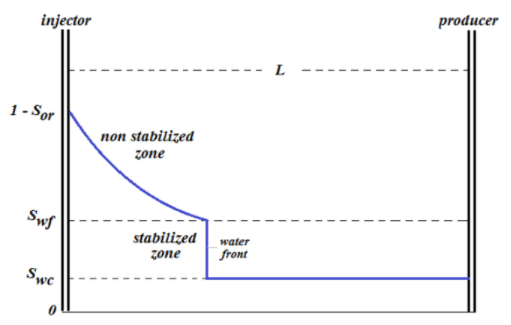
\includegraphics[width=0.5\linewidth]{images/waterflood/saturasiair}

\}

\textbackslash caption\{Profil saturasi air di reservoir selama periode \emph{waterflooding}\}\label{fig:unnamed-chunk-48}
\textbackslash end\{figure\}

~

Dari gambar (2) di atas, terlihat bahwa interval nilai saturasi air diantara \emph{S\textsubscript{wc}} dan \emph{S\textsubscript{wf}} memiliki profil yang sama, yaitu garis lurus vertikal. Hal ini berarti semua nilai saturasi yang berada di antara \emph{S\textsubscript{wc}} dan \emph{S\textsubscript{wf}} (\emph{S\textsubscript{wc}} \textless{} \emph{S\textsubscript{w}} \textless{} \emph{S\textsubscript{wf}}) bergerak dengan kecepatan yang sama, yaitu kecepatan \emph{flood} \emph{front} (atau kecepatan \emph{shock}) yang dinyatakan oleh:
\[(v)_{S_{wc} < S_w < S_{wf}} = \frac{q_t}{A\phi} \left( \frac{\partial f_w}{\partial S_w} \right)_{S_{wf}}\]
Sehingga jarak tempuh dari setiap nilai saturasi dalam interval ini adalah sama, yaitu
\[(x)_{S_{wc} < S_w < S_{wf}} = \frac{q_tt}{A\phi} \left( \frac{\partial f_w}{\partial S_w} \right)_{S_{wf}} = \frac{q_tt}{A\phi} \left( \frac{f_{wf} - f_{wi}}{S_{wf} - S_{wi}} \right)...(23)\]
Zona dimana semua nilai saturasi air dalam interval tersebut bergerak dengan kecepatan yang sama di dalam pori-pori batuan reservoir disebut sebagai zona stabil (\textbf{\emph{stabilized zone}}). Garis biru vertikal pada gambar (2) merupakan \emph{stabilized zone}. Interval nilai saturasi air yang berada di luar interval \emph{stabilized zone} disebut sebagai \emph{non-stabilized zone}, yaitu interval nilai saturasi di atas \emph{S\textsubscript{wf}} (\emph{S\textsubscript{wf}} \textless{} \emph{S\textsubscript{w}} \textless{} 1 − \emph{S\textsubscript{or}}) dimana setiap nilai saturasi air bergerak dengan kecepatan yang berbeda sehingga membentuk profil saturasi air yang tidak konstan. Profil saturasi air untuk interval \_non- \_\_stabilized zone\_ dinyatakan oleh modifikasi dari persamaan (22) untuk interval saturasi air \emph{non-stabilized zone}. Bentuk profil saturasi selama periode injeksi air terdiri atas tiga zona, yaitu \emph{unswept zone} yang memiliki saturasi air \emph{S\textsubscript{wc}}, \emph{stabilized} \emph{zone} dengan nilai saturasi air \emph{S\textsubscript{wf}}, dan \emph{non-stabilized zone} dengan nilai saturasi air yang berubah-ubah antara \emph{S\textsubscript{wf}} dan (1 -- \emph{S\textsubscript{or}}).

\begin{figure}

{\centering 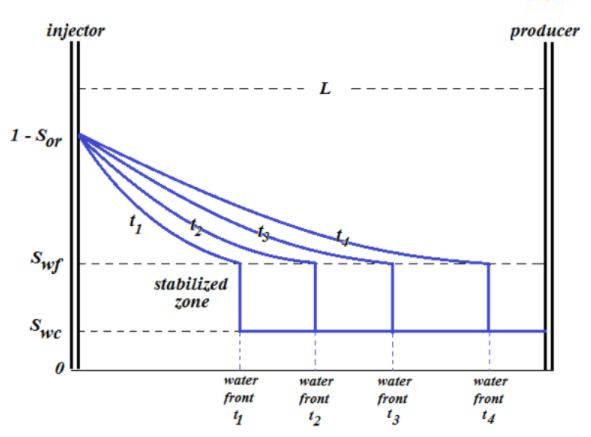
\includegraphics[width=0.5\linewidth]{images/waterflood/saturasiair2} 

}

\caption{Profil saturasi air di reservoir seiring dengan berjalannya waktu}\label{fig:unnamed-chunk-49}
\end{figure}

~

Profil saturasi air di reservoir selama periode \emph{flooding} dapat diketahui dengan menggunakan persamaan (22) dan (23). Penggunaan kedua persamaan ini membutuhkan informasi mengenai nilai turunan \emph{fractional} \emph{flow} terhadap saturasi air, yaitu \(\left( \frac{\partial f_w}{\partial S_w} \right)_{S_w}\) dan \(\left( \frac{\partial f_w}{\partial S_w} \right)_{S_{wf}}\). Nilai kedua parameter ini dapat diperoleh dengan melakukan analisis grafik terhadap kurva \emph{fractional} \emph{flow} \emph{of} \emph{water}, yaitu kurva \emph{f\textsubscript{w}} versus \emph{S\textsubscript{w}}. Berikut akan diberikan penjelasan mengenai hal ini.

Tinjau interval nilai saturasi air antara \emph{S\textsubscript{wc}} dan \emph{S\textsubscript{wf}}. Pada interval ini, semua nilai saturasi air bergerak dengan kecepatan yang sama, yaitu kecepatan \emph{flood front}. Garis lurus yang ditarik dari Swc dan menyinggung kurva \emph{fractional flow water} menyatakan parameter \(\left( \frac{\partial f_w}{\partial S_w} \right)_{S_{wf}}\), sehingga koordinat titik singgung garis ini terhadap kurva \emph{f\textsubscript{w}} merupakan koordinat dari \emph{front water}, yaitu (\emph{S\textsubscript{wf}}, \emph{f\textsubscript{wf}}). Dari analisis grafik ini, nilai \emph{S\textsubscript{wf}} dan \emph{f\textsubscript{wf}} dapat diketahui sehingga persamaan (23) dapat digunakan untuk mendapatkan profil saturasi air untuk interval \emph{S\textsubscript{wc}} \textless{} \emph{S\textsubscript{w}} \textless{} \emph{S\textsubscript{wf}}.

Analisis grafik yang serupa juga berlaku untuk interval \emph{non-stabilized zone}, yaitu interval saturasi air \emph{S\textsubscript{wf}} \textless{} \emph{S\textsubscript{w}} \textless{} \emph{S\textsubscript{or}}. Titik singgung terhadap kurva \emph{f\textsubscript{w}} dari setiap nilai saturasi air yang dipilih pada interval ini (dilambangkan \emph{S\textsubscript{w2}}) akan memberikan nilai fraksi aliran air yang bersesuaian, yaitu \emph{f\textsubscript{w2}}. Dengan diketahuinya nilai (\emph{f\textsubscript{w2}},\emph{S\textsubscript{w2}}), maka modifikasi dari persamaan (22) dapat digunakan untuk mendapatkan profil saturasi air pada interval ini, yaitu:
\[(x)_{S_{w2}} = \frac{q_tt}{A\phi} \left( \frac{\partial f_w}{\partial S_w} \right)_{S_{w2}} = \frac{q_tt}{A\phi} \left( \frac{f_{w2} - f_{wi}}{S_{w2} - S_{wi}} \right)...(24)\]
Konsep analisis grafik untuk menentukan nilai \(\left( \frac{\partial f_w}{\partial S_w} \right)_{S_{wf}}\) dan \(\left( \frac{\partial f_w}{\partial S_w} \right)_{S_{w2}}\) diperlihatkan pada kedua gambar berikut.

\textbackslash begin\{figure\}

\{\centering 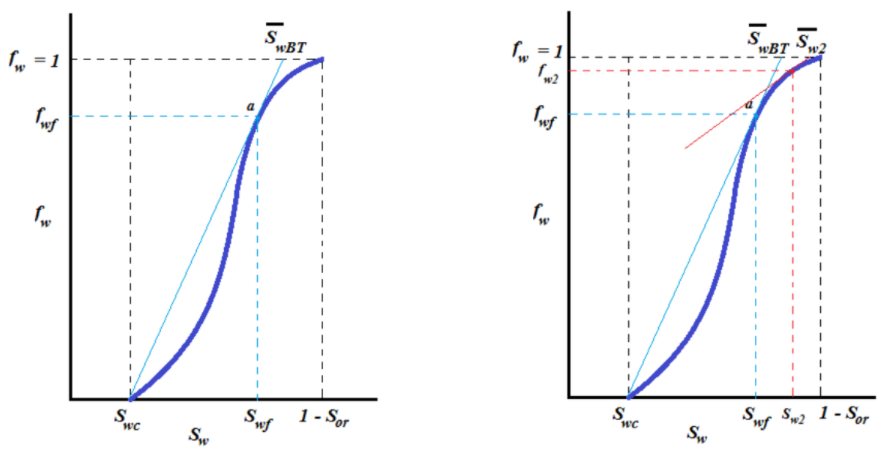
\includegraphics[width=0.75\linewidth]{images/waterflood/perbandingan}

\}

\textbackslash caption\{Analisis grafik pada kurva \emph{f\textsubscript{w}} untuk menentukan nilai \(\left( \frac{\partial f_w}{\partial S_w} \right)_{S_{wf}}\) dan \(\left( \frac{\partial f_w}{\partial S_w} \right)_{S_{w2}}\)\}\label{fig:unnamed-chunk-50}
\textbackslash end\{figure\}

~

Analisis grafik untuk menentukan \(\left( \frac{\partial f_w}{\partial S_w} \right)_{S_w}\) merupakan metode dasar dari teori frontal advance dan diberikan penjelasannya sebagai dasar teori. Pada penelitian ini, metode grafik tidak digunakan. Approksimasi dari nilai \(\left( \frac{\partial f_w}{\partial S_w} \right)_{S_w}\) ditentukan dengan menggunakan metode numerik. Subbab selanjutnya akan membahas mengenai hal ini.

\hypertarget{penentuan-parameter-left-fracpartial-f_wpartial-s_w-right_s_w-dan-saturasi-air-rata-rata-reservoir-bar-s_w}{%
\subsection{\texorpdfstring{Penentuan parameter \(\left( \frac{\partial f_w}{\partial S_w} \right)_{S_w}\) dan Saturasi Air Rata-Rata Reservoir (\(\bar S_w\))}{Penentuan parameter \textbackslash left( \textbackslash frac\{\textbackslash partial f\_w\}\{\textbackslash partial S\_w\} \textbackslash right)\_\{S\_w\} dan Saturasi Air Rata-Rata Reservoir (\textbackslash bar S\_w)}}\label{penentuan-parameter-left-fracpartial-f_wpartial-s_w-right_s_w-dan-saturasi-air-rata-rata-reservoir-bar-s_w}}

Untuk melakukan analisis prediksi performa \emph{waterflooding}, informasi penting yang perlu diketahui selain parameter \(\left( \frac{\partial f_w}{\partial S_w} \right)_{S_w}\) adalah nilai saturasi air rata-rata di reservoir selama periode flooding \(\bar S_w\). Nilai dari \(\bar S_w\) di setiap periode injeksi akan digunakan dalam perhitungan parameter-parameter performa \emph{flooding}.

\hypertarget{metode-numerik-untuk-menentukan-nilai-left-fracpartial-f_wpartial-s_w-right_s_w}{%
\subsubsection{\texorpdfstring{Metode Numerik Untuk Menentukan Nilai \(\left( \frac{\partial f_w}{\partial S_w} \right)_{S_w}\)}{Metode Numerik Untuk Menentukan Nilai \textbackslash left( \textbackslash frac\{\textbackslash partial f\_w\}\{\textbackslash partial S\_w\} \textbackslash right)\_\{S\_w\}}}\label{metode-numerik-untuk-menentukan-nilai-left-fracpartial-f_wpartial-s_w-right_s_w}}

Seperti yang telah diutarakan pada subbab sebelumnya, nilai dari parameter \(\left( \frac{\partial f_w}{\partial S_w} \right)_{S_w}\) penting untuk diketahui karena akan digunakan dalam persamaan (22), (23), dan (24) untuk menghitung profil saturasi air di reservoir. Selain itu, parameter ini pun akan banyak digunakan dalam persamaan-persamaan mengenai parameter performa \emph{flooding} lainnya.

Penelitian ini menggunakan hampiran numerik untuk mencari nilai dari \(\left( \frac{\partial f_w}{\partial S_w} \right)_{S_w}\) persamaan hampiran yang digunakan adalah sebagai berikut.
\[k_{ro} = \alpha _1 (1-S_{wD})^m\]
\[k_{ro} = \alpha _1 S_{wD}^n\]
\[\left( \frac{\partial f_w}{\partial S_w} \right)_{S_w} = \frac{f_{S_w}-f_{S_{wi}}}{S_w - S_{wi}} ...(26) \]
\[f_w = \frac{S_{wD}^n}{[S_{wD}^n\ + A(1-S_{wD})^m ]}...(27)\]
\[\frac{\partial f_w}{\partial S_w} = \frac{AB[nS_{wD}^{n-1}(1-S_{wD})^m\ + S_{wD}^n(1-S_{wD})^{m-1}]}{[S_{wD}^n\ + A(1-S_{wD})^m ]^2}...(28)\]
Dimana \emph{S\textsubscript{wD}} adalah nilai air \emph{dimensionless}, \(\alpha _1\), \(\alpha _2\), \(n\), dan \(m\) adlah koefisien-koefisien numerik.
\[A = \frac{\alpha _1}{\alpha _2}\frac{\mu_w}{\mu_o};B = \frac{1}{1-S_{or}-S_{wi}}\]
\[S_{wD} = \frac{S_{w}-S_{wi}}{1-S_{or}-S_{wi}} = B(S_{w}-S_{wi})...(29)\]
Substitusi persamaan (28) ke persamaan (26)
\[ \frac{f_{S_w}-f_{S_{wi}}}{S_w - S_{wi}} = \frac{AB[nS_{wD}^{n-1}(1-S_{wD})^m\ + S_{wD}^n(1-S_{wD})^{m-1}]}{[S_{wD}^n\ + A(1-S_{wD})^m ]^2} \]
\[ \frac{f_{S_w}}{S_w - S_{wi}} = \frac{AB[nS_{wD}^{n-1}(1-S_{wD})^m\ + S_{wD}^n(1-S_{wD})^{m-1}]}{[S_{wD}^n\ + A(1-S_{wD})^m ]^2} \]
Substitusi pernyataan \emph{f\textsubscript{Sw}} dari persamaan (27),
\[  \frac{\left( \frac{S_{wD}^n}{[S_{wD}^n\ + A(1-S_{wD})^m ]}\right)}  {S_w - S_{wi}} = \frac{AB[nS_{wD}^{n-1}(1-S_{wD})^m\ + S_{wD}^n(1-S_{wD})^{m-1}]}{[S_{wD}^n\ + A(1-S_{wD})^m ]^2} \]
Substitusi pernyataan \emph{S\textsubscript{w}} dari persamaan (29),
\[  \frac{\left( \frac{S_{wD}^n}{[S_{wD}^n\ + A(1-S_{wD})^m ]}\right)}  {\left(\frac{S_{wD}}{B} + S_{wi} \right) - S_{wi}} = \frac{AB[nS_{wD}^{n-1}(1-S_{wD})^m\ + S_{wD}^n(1-S_{wD})^{m-1}]}{[S_{wD}^n\ + A(1-S_{wD})^m ]^2} \]
\[S_{wD}^n\ + A(1-S_{wD})^m = AnS_{wD}^{n-1}(1-S_{wD})^m\ + AmS_{wD}^n(1-S_{wD})^{m-1} \]
\[A(1-S_{wD})^m[nS_{wD}^{n-1}-1]\ + S_{wD}^n[Am(1-S_{wD})^{m-1}-1] = 0 ...(30)\]

~

Solusi dari persamaan (30) untuk \emph{S\textsubscript{wD}} dapat diperoleh secara iterasi numerik menggunakan \textbf{metode Newton} dengan mendefinisikan fungsi berikut:
\[g(S_{wD}) = A(1-S_{wD})^m[nS_{wD}^{n-1}-1]\ + S_{wD}^n[Am(1-S_{wD})^{m-1}-1]\]
Jika \emph{E} melambangkan batas toleransi \emph{error} dari solusi, maka metode Newton diterapkan dengan mengulangi langkah berikut untuk \emph{k} = 1, 2 \ldots{} sampai diperoleh \textbar(S\textsubscript{wD})\textsubscript{k+1} - (S\textsubscript{wD})\textsubscript{k}\textbar{} \textless{} \textsubscript{E}. Nilai \textsubscript{E} yang digunakan adalah 10\textsuperscript{-7}.
\[(S_{wD})_{k+1} = S_{wD})_k - \frac{g((S_{wD})_k)}{g'((S_{wD})_k)}...(31)\]

~

Setelah solusi \emph{S\textsubscript{wD}} diperoleh, lakukan substitusi ke persamaan (27), (28), dan (29), untuk mendapatkan nilai dari \emph{f\textsubscript{w}}, \(\left( \frac{\partial f_w}{\partial S_w} \right)_{S_w}\), dan \emph{S\textsubscript{w}}. Maka persamaan (22) dapat digunakan untuk mendapatkan profil saturasi air. Prosedur numerik yang sama berlaku dalam oenentuan oarameter-parameter \emph{front saturation}, yaitu \emph{f\textsubscript{wf}}, \emph{S\textsubscript{wf}}, dan \(\left( \frac{\partial f_w}{\partial S_w} \right)_{S_wf}\).

\hypertarget{penentuan-nilai-saturasi-air-rata-rata-di-reservoir-selama-periode-waterflooding}{%
\subsubsection{\texorpdfstring{Penentuan Nilai Saturasi Air Rata-Rata di Reservoir Selama Periode \emph{Waterflooding}}{Penentuan Nilai Saturasi Air Rata-Rata di Reservoir Selama Periode Waterflooding}}\label{penentuan-nilai-saturasi-air-rata-rata-di-reservoir-selama-periode-waterflooding}}

Nilai saturasi air rata-rata di reservoir (\(\bar S_w\)) untuk periode tertentu selama proses \emph{waterflooding} dapat ditentukan dengan dua cara, yaitu analisis grafik dan analisis numerik. Penentuan nilai \(\bar S_w\) dari analisis grafik diperlihatkan pada gambar (4). Titik potong garis singgung dengan kurva \emph{f\textsubscript{w}} di nilai \emph{f\textsubscript{w}} = 1 memberikan nilai saturasi air rata-rata di reservoir, \(\bar S_w\). Untuk periode sebelum dan saat terjadi \emph{water breakthrough}, nilai saturasi air rata-rata di reservoir dinyatakan oleh \(\bar S_{wBT}\), sedangkan nilai saturasi air rata-rata di reservoir setelah periode \emph{water breakthrough} dinyatakan oleh \(\bar S_{w2}\).

Metode penentuan nilai \(\bar S_w\) yang digunakan pada penelitian ini adalah metode numerik. Penurunan dari persamaan hampiran numerik yang akan digunakan untuk menentukan \(\bar S_w\) adalah sebagai berikut.

Nilai saturasi air rata-rata di posisi antara x\textsubscript{1} dan x\textsubscript{2}, (x\textsubscript{1} \(\leq\) x \(\leq\) x\textsubscript{2}) dinyatakan oleh:
\[\bar S_w = \frac{\int_{x_1}^{x_2}S_wA\phi dx}{\int_{x_1}^{x_2}A\phi dx}\]
\[\bar S_w = \frac{\int_{x_1}^{x_2}S_w dx}{x_1-x_2}...(32)\]
Tinjau turunan dari \emph{d(xS\textsubscript{w})}:
\[d(xS_w) = S_wdx + xdS_w\]
\[S_wdx = d(xS_w) - xdS_w...(33)\]
Substitusi persamaan (33) ke persamaan (32),
\[\bar S_w = \frac{1}{x_1 - x_2} \int_1^2 d(xS_w)-xdS_w\]
\[\bar S_w = \left[ \frac{1}{x_1 - x_2} \int_{x_1S_{w1}}^{x_2S_{w2}} d(xS_w) \right]-\left[ \frac{1}{x_1 - x_2} \int_{1}^{2} xdS_w \right]\]
\[\bar S_w = \frac{x_2S_{w2}-x_1S_{w1}}{x_2-x_1}-\frac{1}{x_2-x_1}\int_1^2xdS_w ...(34)\]
Subtitusi persamaan (22) ke persamaan (34),
\[\bar S_w = \frac{x_2S_{w2}-x_1S_{w1}}{x_2-x_1}-\frac{1}{x_2-x_1}\int_1^2\frac{q_tt}{A\phi} \left( \frac{\partial f_w}{\partial S_w} \right)_{S_w}dS_w\]
\[\bar S_w = \frac{x_2S_{w2}-x_1S_{w1}}{x_2-x_1}-\frac{q_tt}{A\phi}\frac{1}{x_2-x_1}\int_1^2 df_w\]
\[\bar S_w = \frac{x_2S_{w2}-x_1S_{w1}}{x_2-x_1}-\left( \frac{q_tt}{A\phi} \right)\frac{1}{x_2-x_1}\int_1^2 df_w\]
\[\bar S_w = \frac{x_2S_{w2}-x_1S_{w1}}{x_2-x_1}-\left( \frac{q_tt}{A\phi} \right) \left(\frac{f_{w2}-f_{w1}}{x_2-x_1} \right)....(35)\]
Persamaan (35) merupakan persamaan hampiran umum yang digunakan untuk menghitung nilai saturasi air rata-rata di reservoir pada periode tertentu selama waterflooding. Persamaan (35) dapat dibagi atas perhitungan \(\bar S_w\) sebelum dan saat terjadi \emph{water breakthrough}, dan perhitungan \(\bar S_w\) setelah \emph{water breakthrough}.

Sebelum dan saat \emph{water breakthrough} terjadi, nilai saturasi air rata-rata di reservoir dinyatakan oleh \emph{S\textsubscript{wBT}}. Posisi 1 (\emph{x\textsubscript{1}}) adalah sumur injeksi dan posisi 2 (\emph{x\textsubscript{2s}}) adalah sumur produksi, sehingga pada persamaan (5), \emph{S\textsubscript{w1}} menyatakan nilai saturasi air di sumur injeksi dan \emph{S\textsubscript{w2}} menyatakan nilai saturasi air di sumur produksi. Untuk periode sebelum dan saat \emph{water breakthrough} terjadi, \emph{S\textsubscript{w2}} menyatakan nilai saturasi air di sumur produksi saat terjadi \emph{water breakthrough}, yaitu \emph{S\textsubscript{wBT}} atau \emph{S\textsubscript{wf}} (nilai saturasi air di sumur produksi saat water breakthrough sama dengan nilai saturasi air \emph{flood front}, karena saat terjadi \emph{water breakthrough}, flood front sudah mencapai sumur produksi). Maka, persamaan (5) menjadi:

\[\bar S_{wBT} = \frac{LS_{wBT}}{L} - \left( \frac{q_tt}{A\phi} \right) \left( \frac{f_{wBT}-1}{L} \right) = \bar S_{wBT} -\left( \frac{q_tt}{A\phi L} \right)(f_{wBT}-1)\]
\[\bar S_{wBT} = \left( \frac{q_tt}{A\phi L} \right)(f_{wBT}-1)...(36)\]
Nilai saturasi air rata-rata di reservoir pada periode sebelum dan saat \emph{water breakthrough} dapat dihitung menggunakan persamaan (36). Nilai \emph{S\textsubscript{wf}} dan \emph{f\textsubscript{wf}} diperoleh dari metode numerik yang telah dijelaskan sebelumnya.

Dengan cara yang sama, nilai saturasi air rata-rata di reservoir setelah periode \emph{water breaktrhough} (\(\bar S_{w2}\)) dapat dihitung menggunakan persamaan berikut:
\[\bar S_{w2} = S_{w2}-\left( \frac{q_tt}{A\phi L} \right)(f_{wBT}-1)...(37)\]
dimana \emph{S\textsubscript{w2}} adalah nilai saturasi air di sumur produksi setelah periode \emph{water breakthrough}.

Gambar berikut memperlihatkan konsep saturasi air rata-rata di reservoir pada periode sebelum dan saat terjadi \emph{water breakthrough}, dan periode setelah \emph{water breakthrough}. Gambar di bawah juga memperlihatkan nilai saturasi air di sumur injeksi dan sumur produksi untuk kedua periode ini.

\textbackslash begin\{figure\}

\{\centering 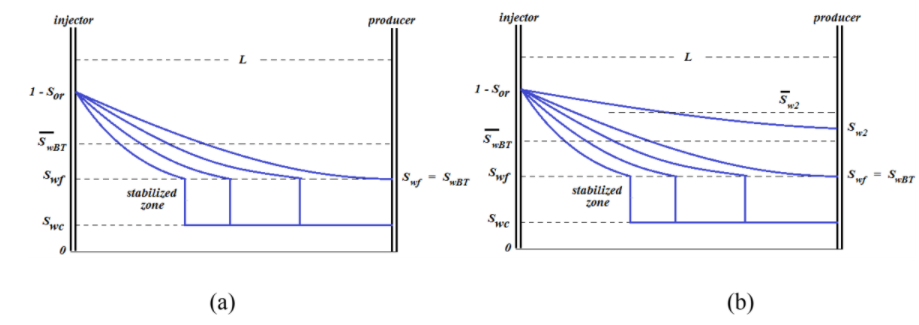
\includegraphics[width=0.75\linewidth]{images/waterflood/saturasi3}

\}

\textbackslash caption\{(a) Profil saturasi air di reservoir sebelum sampai saat terjadi water breakthrough dengan \textbf{\(\bar S_{wBT}\)} menyatakan nilai saturasi air rata-rata di reservoir selama periode ini terjadi;(b) Profil saturasi air setelah periode water breakthrough dengan \textbf{\(\bar S_{w2}\)} menyatakan nilai saturasi air rata-rata di reservoir selama periode ini\}\label{fig:unnamed-chunk-51}
\textbackslash end\{figure\}

~

\hypertarget{penentuan-parameter-efisiensi-waterflooding}{%
\section{\texorpdfstring{Penentuan Parameter Efisiensi \emph{Waterflooding}}{Penentuan Parameter Efisiensi Waterflooding}}\label{penentuan-parameter-efisiensi-waterflooding}}

Prediksi performa reservoir di bawah proses waterflood dilakukan melalui perhitungan terhadap tiga parameter efisiensi \emph{flooding}, yaitu \textbf{\emph{displacement efficiency (E\emph{D}), areal sweep efficiency (E\emph{A}), dan vertical sweep efficiency (E\emph{V})}}. Ketiga parameter efisiensi di atas merupakan parameter yang berlaku baik pada proses \emph{secondary recovery} maupun \emph{tertiary recovery}. Nilai dari ketiga parameter efisiensi di atas akan meningkat selama proses \emph{waterflood} dilakukan dan akan mencapai nilai maksimum di economic limit dari proyek \emph{waterflood.} Berikut akan diberikan penjelasan singkat dari ketiga parameter ini.

\hypertarget{displacement-efficiency-ed}{%
\subsection{\texorpdfstring{\emph{Displacement Efficiency} (E\textsubscript{D})}{Displacement Efficiency (ED)}}\label{displacement-efficiency-ed}}

\emph{Displacement efficiency (E\textsubscript{D})} merupakan parameter yang menyatakan fraksi minyak residu yang telah tersapu oleh fluida injeksi setiap waktu. Persamaan untuk menghitung \emph{E\textsubscript{D}} adalah:
\[E_D = \frac{volume\ minyak\ saat\ awal\ flooding\ - volume\ minyak\ residu}{volume\ minyak\ saat\ awal\ flooding}\]
\[E_D = \frac{(pore\ volume)(\frac{S_{oi}}{B_{oi}})-(pore\ volume)(\frac{S_{o}}{B_{o}})}{(pore\ volume)(\frac{S_{oi}}{B_{oi}})} = \frac{\frac{S_{oi}}{B_{oi}}-\frac{\bar S_{o}}{B_{o}}}{\frac{S_{oi}}{B_{oi}}}\]
Dengan mengasumsikan nilai konstan dari faktor volue formasi minyak, persamaan di atas menjadi:
\[E_D = \frac{S_{oi}-S_{oi}}{\bar S_{o}}=\frac{\bar S_{w} - S_{wi} - S_{gi}}{1 - S_{wi} - S_{gi}}...(38)\]
Jika tidak terdapat \emph{initial gas saturation} (\emph{S\textsubscript{gi}} = 0) saat awal \emph{flooding},
\[E_D = \frac{\bar S_{w} - S_{wi}}{1-S_{wi}}\]

\hypertarget{areal-sweep-efficiency-ea}{%
\subsection{\texorpdfstring{\emph{Areal Sweep Efficiency} (E\textsubscript{A})}{Areal Sweep Efficiency (EA)}}\label{areal-sweep-efficiency-ea}}

\emph{Areal sweep efficiency} (\emph{E\textsubscript{A}}) merupakan parameter yang menyatakan fraksi total area injeksi yang telah tersapu oleh fluida injeksi. Nilai \emph{E\textsubscript{A}} bergantung pada beberapa parameter, diantaranya \emph{mobility ratio}, pola injeksi yang digunakan, volume air inj\_eksi kumulatif, distribusi tekanan antara sumur injeksi dengan sumur produksi, dan keheterogenan areal. Diantara parameter-parameter ini, \_mobility ratio merupakan parameter yang paling penting.

Mobilitas suatu fluida (dilambangkan \(\lambda\)) didefinisikan sebagai perbandingan antara permeabilitas efektif suatu fasa fluida dengan viskositas fasa fluida tersebut. Mobilitas fluida sangat dipengaruhi oleh saturasi fluida yang bersangkutan. Mobilitas untuk setiap fasa fluida reservoir dinyatakan sebagai berikut.

\[\lambda_o = \frac{k_o}{\mu_o}=\frac{kk_{ro}}{\mu_o}\]
\[\lambda_w = \frac{k_w}{\mu_w}=\frac{kk_{rw}}{\mu_w}\]
\[\lambda_g = \frac{k_g}{\mu_g}=\frac{kk_{rg}}{\mu_g}...(40)\]

~

Dari definisi mobilitas fluida, maka \textbf{\emph{mobility ratio}} (dilambangkan \textbf{\emph{M}}) didefinisikan sebagai perbandingan antara mobilitas fasa fluida injeksi terhadap mobilitas fasa fluida terpindahkan. Dalam hal \emph{waterflooding}, fasa fluida pendorong (fluida injeksi) adalah air dan fasa fluida terpindahkan adalah minyak, sehingga
\[M = \frac{\lambda_{pendorong}}{\lambda_{terpindahkan}}=\frac{\lambda_w}{\lambda_o}=\frac{kk_{rw}}{\mu_w}\frac{\mu_o}{kk_{ro}}=\frac{k_{rw}}{k_{ro}}\frac{\mu_o}{\mu_w}...(41)\]
Perhitungan \emph{M} sepanjang periode \emph{waterflooding} untuk periode sebelum water breakthrough dan setelah \emph{water breakthrough} diberikan oleh persamaan (42) dan (43). Persamaan (42) adalah persamaan yang digunakan untuk menghitung nilai \emph{M} untuk periode awal injeksi hingga \emph{water breakthrough}, sedangkan persamaan (43) adalah persamaan yang digunakan untuk menghitung nilai \emph{M} dari mulai periode \emph{water breakthrough} hingga akhir periode injeksi.
\[M= \frac{k_{rw}@\bar S_{wBT}}{k_{ro}@\bar S_{wi}}\frac{\mu_o}{\mu_w}...(42)\]
\[M= \frac{k_{rw}@\bar S_{w2}}{k_{ro}@\bar S_{wi}}\frac{\mu_o}{\mu_w}...(43)\]
Nilai \emph{E\textsubscript{A}} untuk setiap periode injeksi dinyatakan oleh:
\emph{E\textsubscript{A}} sebelum periode \emph{water breakthrough}:
\[E_A = \frac{W_{inj}}{(PV)(\bar S_{wBT}- S_{wi})}...(44)\]
\emph{E\textsubscript{A}} saat \emph{water breakthrough}:
\[E-A = 0.54602036 + \frac{0.03170817}{M} + \frac{0.30222997}{e^M} - 0.00509693M...(45)\]
\emph{E\textsubscript{A}} setelah periode \emph{water breakthrough}:
\[E_A = E_{ABT} + 0.633log\left( \frac{W-{inj}}{W-{iBT}} \right)\]

atau

\[E_A = E_{ABT} + 0.2749ln\left( \frac{W-{inj}}{W-{iBT}} \right)...(46)\]
\#\#\# \emph{Vertical Sweep Efficiency} (E\textsubscript{V})

\emph{Vertical Sweep Efficiency} \emph{(E\textsubscript{V})} merupakan parameter yang menyatakan fraksi vertikal reservoir yang telah tersentuh oleh fluida injeksi. Variasi permeabilitas secara vertikal merupakan parameter yang pengaruhnya dianggap paling signifikan terhadap nilai \emph{E\textsubscript{V}}.

Dykstra-Parsons menyusun korelasi yang menghubungkan \emph{E\textsubscript{V}} dengan parameter \emph{V\textsubscript{DP}} (koefisien variasi permeabilitas Dykstra-Parsons), \emph{mobility ratio M}, dan \emph{water-oil ratio} (WOR). Korelasi ini dinyatakan dalam bentuk parameter korelasi Y yang dinyatakan sebagai:
\[Y = \frac{(WOR+0.4)(18.948 - 2.499V_{DP})}{(M - 0.8094V_{DP}+1.137)10^x} ...(47)\]
dimana
\[x = 1.6453V^2 + 0.935V - 0.6891\]
Nilai \emph{E\textsubscript{V}} dihitung menggunakan metode iterasi terhadap persamaan berikut:
\[\alpha_1E_V^{\alpha_2}(1-E_V)^{\alpha_3} - y = 0 ...(48)\]
Pada persamaan (48), nilai Y diperoleh dari persamaan (47) sedangkan nilai dari parameter-parameter \(\alpha_1\), \(\alpha_2\), dan \(\alpha_3\) berturut-turut adalah 3.334088568, 0.7737348199, dan 1.225859406.

\hypertarget{persamaan-persamaan-yang-digunakan-dalam-prediksi-performa-waterflooding}{%
\section{\texorpdfstring{Persamaan-Persamaan yang Digunakan Dalam Prediksi Performa \emph{Waterflooding}}{Persamaan-Persamaan yang Digunakan Dalam Prediksi Performa Waterflooding}}\label{persamaan-persamaan-yang-digunakan-dalam-prediksi-performa-waterflooding}}

Beberapa parameter performa \emph{waterflooding} beserta persamaan yang digunakan untuk menghitung parameter tersebut dirangkum pada tabel berikut, dimana masing-masing kolom mewakili dua periode \emph{waterflood}, yaitu periode sebelum \emph{water breakthrough} dan setelah \emph{water breakthrough}.

\begin{longtable}[]{@{}cccc@{}}
\caption{{ Tabel 3.1: Persamaan-persamaan yang digunakan dalam perhitungan performa \emph{waterflood} }}\tabularnewline
\toprule
\begin{minipage}[b]{0.22\columnwidth}\centering
No\strut
\end{minipage} & \begin{minipage}[b]{0.22\columnwidth}\centering
Parameter\strut
\end{minipage} & \begin{minipage}[b]{0.22\columnwidth}\centering
Sebelum dan Saat \emph{Water Breakthrough}\strut
\end{minipage} & \begin{minipage}[b]{0.22\columnwidth}\centering
Setelah \emph{Water Breakthrough}\strut
\end{minipage}\tabularnewline
\midrule
\endfirsthead
\toprule
\begin{minipage}[b]{0.22\columnwidth}\centering
No\strut
\end{minipage} & \begin{minipage}[b]{0.22\columnwidth}\centering
Parameter\strut
\end{minipage} & \begin{minipage}[b]{0.22\columnwidth}\centering
Sebelum dan Saat \emph{Water Breakthrough}\strut
\end{minipage} & \begin{minipage}[b]{0.22\columnwidth}\centering
Setelah \emph{Water Breakthrough}\strut
\end{minipage}\tabularnewline
\midrule
\endhead
\begin{minipage}[t]{0.22\columnwidth}\centering
1\strut
\end{minipage} & \begin{minipage}[t]{0.22\columnwidth}\centering
Jumlah \emph{pore volume}(PV) injeksi air, (\(Q_i\))\strut
\end{minipage} & \begin{minipage}[t]{0.22\columnwidth}\centering
\(Q_{iBT}=\frac{1}{\left( \frac{\partial f_w}{\partial S_w} \right)_{S_{wf}}}=\bar S_{wBT} - S_{wi}\)\strut
\end{minipage} & \begin{minipage}[t]{0.22\columnwidth}\centering
\(Q_i = \frac{1}{\left( \frac{\partial f_w}{\partial S_w} \right)_{S_{w2}}}\)\strut
\end{minipage}\tabularnewline
\begin{minipage}[t]{0.22\columnwidth}\centering
2\strut
\end{minipage} & \begin{minipage}[t]{0.22\columnwidth}\centering
Volume injeksi air kumulatif, (\(W_i\))\strut
\end{minipage} & \begin{minipage}[t]{0.22\columnwidth}\centering
\(W_{iBT} = (PV)(\bar S_{wBT}-S_{wi})E_{ABT}E_{VBT}\) \(W_{iBT}=(PV)Q_{iBT}E_{ABT}E_{VBT}\)\strut
\end{minipage} & \begin{minipage}[t]{0.22\columnwidth}\centering
\(W_{inj}=(PV)(\bar S_{w2}-S_{wi}E_AE_V)\) \(W_{inj} = (PV)Q_iE_AE_V\)\strut
\end{minipage}\tabularnewline
\begin{minipage}[t]{0.22\columnwidth}\centering
3\strut
\end{minipage} & \begin{minipage}[t]{0.22\columnwidth}\centering
\emph{Displacement efficiency} (\(E_D\))\strut
\end{minipage} & \begin{minipage}[t]{0.22\columnwidth}\centering
\(E_{DBT} = \frac{\bar S_{wBT} - S_{wi}}{1-S_{wi}}\)\strut
\end{minipage} & \begin{minipage}[t]{0.22\columnwidth}\centering
\(E_{D} = \frac{\bar S_{w2} - S_{wi}}{1-S_{wi}}\)\strut
\end{minipage}\tabularnewline
\begin{minipage}[t]{0.22\columnwidth}\centering
4\strut
\end{minipage} & \begin{minipage}[t]{0.22\columnwidth}\centering
\emph{Displacement efficiency} (\(E_A\))\strut
\end{minipage} & \begin{minipage}[t]{0.22\columnwidth}\centering
Sebelum BT: persamaan (44) Saat BT: persamaan (45)\strut
\end{minipage} & \begin{minipage}[t]{0.22\columnwidth}\centering
Persamaan (46)\strut
\end{minipage}\tabularnewline
\begin{minipage}[t]{0.22\columnwidth}\centering
5\strut
\end{minipage} & \begin{minipage}[t]{0.22\columnwidth}\centering
\emph{Displacement efficiency} (\(E_V\))\strut
\end{minipage} & \begin{minipage}[t]{0.22\columnwidth}\centering
Persamaan (48)\strut
\end{minipage} & \begin{minipage}[t]{0.22\columnwidth}\centering
Persamaan (48)\strut
\end{minipage}\tabularnewline
\begin{minipage}[t]{0.22\columnwidth}\centering
6\strut
\end{minipage} & \begin{minipage}[t]{0.22\columnwidth}\centering
Waktu \emph{breakthrough}, \emph{t}\strut
\end{minipage} & \begin{minipage}[t]{0.22\columnwidth}\centering
\(t_{BT} = \frac{W_{iBT}}{q_t}=\frac{W_{iBT}}{i_w}\)\strut
\end{minipage} & \begin{minipage}[t]{0.22\columnwidth}\centering
\(t_{BT} = \frac{W_{inj}}{q_t}=\frac{W_{inj}}{i_w}\)\strut
\end{minipage}\tabularnewline
\begin{minipage}[t]{0.22\columnwidth}\centering
7\strut
\end{minipage} & \begin{minipage}[t]{0.22\columnwidth}\centering
Koefisien Variasi Permeabilitas Dystra-Parsons, \(V_{DP}\)\strut
\end{minipage} & \begin{minipage}[t]{0.22\columnwidth}\centering
\(V_{DP}=\frac{k_{50}-k_{84.1}}{k_{50}}\)\strut
\end{minipage} & \begin{minipage}[t]{0.22\columnwidth}\centering
\(V_{DP}=\frac{k_{50}-k_{84.1}}{k_{50}}\)\strut
\end{minipage}\tabularnewline
\begin{minipage}[t]{0.22\columnwidth}\centering
8\strut
\end{minipage} & \begin{minipage}[t]{0.22\columnwidth}\centering
\emph{Mobiity Ratio, M}\strut
\end{minipage} & \begin{minipage}[t]{0.22\columnwidth}\centering
\(M=\frac{k_{rw}@\bar S_{wBT}}{k_{ro}@\bar S_{wi}}\frac{\mu_o}{\mu_w}\)\strut
\end{minipage} & \begin{minipage}[t]{0.22\columnwidth}\centering
\(M=\frac{k_{rw}@\bar S_{w2}}{k_{ro}@\bar S_{wi}}\frac{\mu_o}{\mu_w}\)\strut
\end{minipage}\tabularnewline
\begin{minipage}[t]{0.22\columnwidth}\centering
9\strut
\end{minipage} & \begin{minipage}[t]{0.22\columnwidth}\centering
\emph{Water-Oil-ratio} (WOR)\strut
\end{minipage} & \begin{minipage}[t]{0.22\columnwidth}\centering
Sebelum BT: \emph{WOR} = 0 Saat BT: (\emph{WOR})\textsubscript{s} = \(\frac{B_o}{B_w \left(\frac{1}{f_{wBT}} \right)-1}\)\strut
\end{minipage} & \begin{minipage}[t]{0.22\columnwidth}\centering
(\emph{WOR})\textsubscript{s} = \(\frac{B_o}{B_w \left(\frac{1}{f_{w2}} \right)-1}\)\strut
\end{minipage}\tabularnewline
\begin{minipage}[t]{0.22\columnwidth}\centering
10\strut
\end{minipage} & \begin{minipage}[t]{0.22\columnwidth}\centering
Kumulatif produksi minyak, \(N_p\)\strut
\end{minipage} & \begin{minipage}[t]{0.22\columnwidth}\centering
Saat BT: \(N_{PBT}=N_sE_{DBT}E_{ABT}E_{VBT}\)\strut
\end{minipage} & \begin{minipage}[t]{0.22\columnwidth}\centering
\(N_{P}=N_sE_{D}E_{A}E_{V}\)\strut
\end{minipage}\tabularnewline
\begin{minipage}[t]{0.22\columnwidth}\centering
11\strut
\end{minipage} & \begin{minipage}[t]{0.22\columnwidth}\centering
Kumulatif produksi air, \(W_p\)\strut
\end{minipage} & \begin{minipage}[t]{0.22\columnwidth}\centering
Sebelum BT: \(W_p = 0\)\strut
\end{minipage} & \begin{minipage}[t]{0.22\columnwidth}\centering
\(W_p = \frac{W-{inj}- (N_pB_o)}{B_w}\)\strut
\end{minipage}\tabularnewline
\begin{minipage}[t]{0.22\columnwidth}\centering
12\strut
\end{minipage} & \begin{minipage}[t]{0.22\columnwidth}\centering
Laju produski minyak, \(Q_o\)\strut
\end{minipage} & \begin{minipage}[t]{0.22\columnwidth}\centering
\(Q_o = \frac{q_t}{B_o}=\frac{i_w}{B_o}\)\strut
\end{minipage} & \begin{minipage}[t]{0.22\columnwidth}\centering
\(Q_o=\frac{i_w}{B_o+B_w(WOR)_s}\)\strut
\end{minipage}\tabularnewline
\begin{minipage}[t]{0.22\columnwidth}\centering
13\strut
\end{minipage} & \begin{minipage}[t]{0.22\columnwidth}\centering
Laju produski air, \(Q_w\)\strut
\end{minipage} & \begin{minipage}[t]{0.22\columnwidth}\centering
Sebelum BT: \(Q_w = 0\)\strut
\end{minipage} & \begin{minipage}[t]{0.22\columnwidth}\centering
\(Q_w = Q_o(WOR)_s\)\strut
\end{minipage}\tabularnewline
\bottomrule
\end{longtable}

\hypertarget{persamaan-persamaan-dasar-dan-nilai-default-yang-digunakan-dalam-predictive-model}{%
\section{\texorpdfstring{Persamaan-Persamaan Dasar dan Nilai \emph{Default} yang digunakan Dalam \emph{Predictive Model}}{Persamaan-Persamaan Dasar dan Nilai Default yang digunakan Dalam Predictive Model}}\label{persamaan-persamaan-dasar-dan-nilai-default-yang-digunakan-dalam-predictive-model}}

\hypertarget{viskositas-minyak}{%
\subsection{Viskositas Minyak}\label{viskositas-minyak}}

Viskositas minyak, \(\mu_o\) dihitung menggunakan korelasi Beggs-Robinson. Korelasi Beggs-Robinson terlebih dahulu menghitung nilai viskositas \emph{dead oil}, \(\mu_{od}\).
\[\mu_{od}=10^x-1...(49)\]
dengan:
\[X = \frac{Y}{T^{1.163}}\]
\[Y=10^Z\]
\[Z=3.0324-0.022023(API)\]
Selanjutnya, viskositas \emph{live oil} dihitung dengan menggunakan persamaan berikut.
\[\mu_o= A(\mu_{od})^B...(50)\]
dengan:
\[A=\frac{10.715}{(R_s + 100)^{0.515}}\]
\[B = \frac{5.44}{(R_s + 150)^{0.338}}\]
dimana:
\emph{T} = temperatur reservoir, \(\circ\)F
\emph{R\textsubscript{s}} = \emph{solution gas-oil ratio}, SCF/STB

\hypertarget{solution-gas-oil-ratio}{%
\subsection{\texorpdfstring{\emph{SolUtion Gas-Oil Ratio}}{SolUtion Gas-Oil Ratio}}\label{solution-gas-oil-ratio}}

\emph{Solution gas-oil ratio}, \emph{R\textsubscript{s}}, dihitung menggunakan korelasi Vasquez-Beggs. Dalam korelasi Vasquez-Beggs, nilai s\_pecific gravity gas\_, \(\gamma_g\), terlebih dahulu dikoreksi ke dalam kondisi tekanan \emph{separator} 100 psig dan temperatur \emph{separator} (temperatur \emph{separator} diasumsikan sama dengan temperatur reservoir).
\[\gamma_{g.100} = \gamma_g \left[ 1+\left( (5.912(10)^{-5}(API)(T)log \left( \frac{64.7}{114.7} \right) \right) \right]...(51)\]
Selanjutnya, nilai \emph{soultion gas-oil ratio} dihitung sebagai berikut.
Untuk \emph{API} \(\leq\) 30:
\[R_s = 0.0362 \gamma_{g.100} P_{form}^{1.0937}exp \left[ 25.724 \left( \frac{API}{T+460} \right)\right]...(52)\]
Untuk \emph{API} \textgreater{} 30:
\[R_s = 0.0178 \gamma_{g.100} P_{form}^{1.187}exp \left[ 23.931 \left( \frac{API}{T+460} \right)\right]...(53)\]

\hypertarget{faktor-volume-formasi-minyak}{%
\subsection{Faktor Volume Formasi Minyak}\label{faktor-volume-formasi-minyak}}

Faktor volume formasi minyak, \emph{B\textsubscript{o}}, dihitung menggunakan korelasi Vasquez-Beggs.
\[B_o = 1 + C_1R_s+(C_2+C_3R_s)(T-60) \left( \frac{API}{\gamma_{g.100}} \right) ...(54)\]
dimana:
Untuk \emph{API} \(\leq\) 30:
\[C_1 =4.677(10^{-4})\]
\[C_2 =1.751(10^{-5})\]
\[C_3 =-1.811(10^{-8})\]

\hypertarget{permeabilitas-relatif}{%
\subsection{Permeabilitas Relatif}\label{permeabilitas-relatif}}

Nilai permeabilitas relatif minyak (\emph{k\textsubscript{ro}}) dan air (\emph{k\textsubscript{rw}}) dihitung menggunakan korelasi Corey.
\[u_o = \frac{1-S_{w}-S_{orw}}{1-S_{wc}-S_{orw}}...(55)\]
\[k_{ro}=X_{k_{roe}}u_o^{X_{no}}...(56)\]
\[u_w = \frac{S_{w}-S_{wc}}{1-S_{wc}-S_{orw}}...(57)\]
\[k_{rw}=X_{k_{rwe}}u_w^{X_{nw}}...(58)\]
dimana:
\(S_w\) = saturasi air
\(S_{wc}\) = \emph{connate water saturation}
\(S_{orw}\) = saturasi minyak residu
\(X_{k_{roe}}\) = nilai permeabilitas relatif minyak saat \(S_{wc}\)
\(X_{k_{rwe}}\) = nilai permeabilitas relatif air saat \(S_{orw}\)
\(X_{no}\) = eksponen kurva permeabilitas relatif minyak
\(X_{nw}\) = eksponen kurva permeabilitas relatif air

\hypertarget{nilai-default-parameter-yang-digunakan-dalam-model}{%
\subsection{\texorpdfstring{Nilai \emph{Default} Parameter yang Digunakan Dalam Model}{Nilai Default Parameter yang Digunakan Dalam Model}}\label{nilai-default-parameter-yang-digunakan-dalam-model}}

Tabel berikut merangkum persamaan dan nilai \emph{default} yang digunakan dari sejumlah parameter dalam \emph{predictive model}.

\begin{longtable}[]{@{}cc@{}}
\caption{{ Tabel 3.2: Nilai \emph{default} yang digunakan dari sejumlah parameter dalam \emph{predictive model} }}\tabularnewline
\toprule
\begin{minipage}[b]{0.47\columnwidth}\centering
Parameter\strut
\end{minipage} & \begin{minipage}[b]{0.47\columnwidth}\centering
Nilai \emph{Default} yang Digunakan\strut
\end{minipage}\tabularnewline
\midrule
\endfirsthead
\toprule
\begin{minipage}[b]{0.47\columnwidth}\centering
Parameter\strut
\end{minipage} & \begin{minipage}[b]{0.47\columnwidth}\centering
Nilai \emph{Default} yang Digunakan\strut
\end{minipage}\tabularnewline
\midrule
\endhead
\begin{minipage}[t]{0.47\columnwidth}\centering
Tekanan formasi, \(P_{form}\)\strut
\end{minipage} & \begin{minipage}[t]{0.47\columnwidth}\centering
\(P_{form}=15+0.433 (depth)\)\strut
\end{minipage}\tabularnewline
\begin{minipage}[t]{0.47\columnwidth}\centering
Temperatur formasi, \(T\)\strut
\end{minipage} & \begin{minipage}[t]{0.47\columnwidth}\centering
\(T=60+0.017(depth)\)\strut
\end{minipage}\tabularnewline
\begin{minipage}[t]{0.47\columnwidth}\centering
\emph{Specific gravity gas}, \(\gamma_g\)\strut
\end{minipage} & \begin{minipage}[t]{0.47\columnwidth}\centering
\(\gamma_g = 0.8\)\strut
\end{minipage}\tabularnewline
\begin{minipage}[t]{0.47\columnwidth}\centering
Koefisien variasi permeabilitas Dystra-Parsons, \(V_{DP}\)\strut
\end{minipage} & \begin{minipage}[t]{0.47\columnwidth}\centering
\(V_{DP}=0.72\)\strut
\end{minipage}\tabularnewline
\begin{minipage}[t]{0.47\columnwidth}\centering
Jumlah lapisan reservoir\strut
\end{minipage} & \begin{minipage}[t]{0.47\columnwidth}\centering
Minimum = 1 Maksimum = 10\strut
\end{minipage}\tabularnewline
\begin{minipage}[t]{0.47\columnwidth}\centering
Faktor volume formasi air, \(B_w\)\strut
\end{minipage} & \begin{minipage}[t]{0.47\columnwidth}\centering
Korelasi Keenan dan Keyes: \(B_w=1+1.2(10^{-4})(T-60)+1(10^{-6})(T-60)^2-3.33(10^{-6})P_{form}\)\strut
\end{minipage}\tabularnewline
\begin{minipage}[t]{0.47\columnwidth}\centering
Viskositas air, \(\mu_w\)\strut
\end{minipage} & \begin{minipage}[t]{0.47\columnwidth}\centering
Korelasi Van Wingen: \(\mu_w = exp[1.003-1.479(10^{-2})T+1.982(10^{-5})T^2]\)\strut
\end{minipage}\tabularnewline
\begin{minipage}[t]{0.47\columnwidth}\centering
\emph{Connate water saturation}, \(S_{wc}\)\strut
\end{minipage} & \begin{minipage}[t]{0.47\columnwidth}\centering
\(S_{wc}=0.3\)\strut
\end{minipage}\tabularnewline
\begin{minipage}[t]{0.47\columnwidth}\centering
Saturasi minyak residu, \(S_{orw}\)\strut
\end{minipage} & \begin{minipage}[t]{0.47\columnwidth}\centering
Untuk tipe batuan \emph{sandstone}, \(S_{orw}=0.25\) Untuk tipe batuan karbonat, \(S_{orw}=0.38\)\strut
\end{minipage}\tabularnewline
\begin{minipage}[t]{0.47\columnwidth}\centering
Permeabilitas relatif minyak saat \(S_{wc}\), \(X_{k_{roe}}\)\strut
\end{minipage} & \begin{minipage}[t]{0.47\columnwidth}\centering
Untuk tipe batuan \emph{sandstone}, \(X_{k_{roe}}=0.8\) Untuk tipe batuan karbonat, \(X_{k_{roe}}=0.4\)\strut
\end{minipage}\tabularnewline
\begin{minipage}[t]{0.47\columnwidth}\centering
Permeabilitas relatif air saat \(S_{orw}\), \(X_{k_{rwe}}\)\strut
\end{minipage} & \begin{minipage}[t]{0.47\columnwidth}\centering
Untuk tipe batuan \emph{sandstone}, \(X_{k_{rwe}}=0.2\) Untuk tipe batuan karbonat, \(X_{k_{rwe}}=0.3\)\strut
\end{minipage}\tabularnewline
\begin{minipage}[t]{0.47\columnwidth}\centering
Eksponen kurva permeabilitas relatif minyak, \(X_{no}\)\strut
\end{minipage} & \begin{minipage}[t]{0.47\columnwidth}\centering
\(X_{no}=2\)\strut
\end{minipage}\tabularnewline
\begin{minipage}[t]{0.47\columnwidth}\centering
Eksponen kurva permeabilitas relatif air, \(X_{nw}\)\strut
\end{minipage} & \begin{minipage}[t]{0.47\columnwidth}\centering
\(X_{nw}=2\)\strut
\end{minipage}\tabularnewline
\begin{minipage}[t]{0.47\columnwidth}\centering
Radius sumur, \(r_w\)\strut
\end{minipage} & \begin{minipage}[t]{0.47\columnwidth}\centering
\(r_w=0.5ft\)\strut
\end{minipage}\tabularnewline
\bottomrule
\end{longtable}

\hypertarget{chemical-flood-predictive-model}{%
\chapter{Chemical Flood Predictive Model}\label{chemical-flood-predictive-model}}

\hypertarget{pendahuluan-2}{%
\section{Pendahuluan}\label{pendahuluan-2}}

Injeksi kimia (\emph{chemical flooding}) merupakan bagian dari metode \emph{Enhanced Oil Recovery} (EOR)yang menggunakan injeksi larutan kimia yang akan bereaksi secara kimiawi (\emph{chemical liquid}) di reservoir. Zat kimia yang umumnya digunakan adalah surfaktan, polimer, dan alkali. \emph{Chemical flooding} dapat dibedakan berdasarkan tipe zat kimia yang digunakan, diantaranya injeksi polimer, injeksi surfaktan, injeksi alkali (disebut juga \emph{caustic flooding}), injeksi surfaktan-polimer (disebut juga \emph{micellar flooding}), injeksi alkali-polimer (disebut juga \emph{caustic-polymer flooding}), dan injeksi alkali-surfaktan-polimer (\emph{ASP flooding}).

Laporan ini membahas mengenai penyusunan \emph{chemical flood predictive model} untuk memprediksi performa reservoir di bawah pengaruh injeksi kimia. Tipe injeksi kimia yang ditinjau dalam model adalah injeksi surfaktan-polimer (\emph{micellar-polymer} (MP) \emph{flood}), injeksi alkali (\emph{caustic flood}), dan injeksi alkali-polimer (\emph{caustic-polymer flood}). Dalam \emph{predictive model}, \emph{chemical flood} diasumsikan terjadi setelah penerapan \emph{waterflood}, sehingga \emph{chemical flood} dipandang sebagai proses perolehan tersier.

Injeksi surfaktan-polimer (MP \emph{flood}) ditentukan sebagai model default dalam \emph{predictive model}, dengan dua pilihan metode lainnya, yaitu \emph{caustic flood }dan \emph{caustic-polymer flood}, dimana perhitungan prediksi performa dari \emph{caustic} dan \emph{caustic-polymer flood} ditentukan berdasarkan performa dari MP \emph{flood}, yaitu masing-masing sebesar 15\% dan 40\% dari nilai prediksi MP \emph{flood} untuk parameter perolehan minyak.

Algoritma \emph{predictive model} dibangun dari tinjauan teori dan studi simulasi. Terdapat sejumlah faktor yang pengaruhnya dianggap paling signifikan terhadap performa produksi MP \emph{flood}. Faktor-faktor ini diantaranya adalah bilangan kapiler (\emph{capillary number}), keheterogenan reservoir (\emph{reservoir heterogeneity}), \emph{crossflow}, adsorpsi surfaktan pada batuan formasi, dan \emph{wettability}.

Teori \emph{fractional flow} digunakan untuk melakukan analisis terhadap beberapa parameter performa \emph{flooding}, seperti \emph{oil breakthrough}, \emph{surfactant breakthrough}, perolehan minyak (\emph{oil recovery}), dan \emph{project life}. Efisiensi perolehan minyak (\emph{oil recovery efficiency}) ditentukan sebagai hasil kali antara \emph{displacement efficiency} (\emph{E\textsubscript{D}}), \emph{vertical sweep efficiency} dari surfaktan (\emph{E\textsubscript{V}}), dan \emph{polymer sweep} atau \emph{mobility buffer} \emph{sweep efficiency} (\emph{E\textsubscript{MB}}). Koreksi adanya \emph{crossflow} terhadap nilai efisiensi perolehan minyak dilakukan melalui korelasi yang merupakan fungsi dari rasio \(\frac{k_v}{k_h}\).

\emph{Displacement efficiency} ditentukan dari korelasi yang merupakan fungsi dari bilangan kapiler, sedangkan \emph{vertical sweep efficiency} dihitung menggunakan korelasi yang diperoleh dari studi simulasi. Korelasi ini merupakan fungsi dari ukuran injeksi \emph{slug} surfaktan, adsorpsi surfaktan pada batuan formasi, dan keheterogenan reservoir. \emph{Polymer sweep} juga ditentukan berdasarkan korelasi dari hasil simulasi. Korelasi yang dibangun merupakan fungsi dari ukuran \emph{slug} injeksi polimer dan \emph{vertical sweep efficienc}y.

Efek keheterogenan reservoir terhadap kecepatan \emph{front} surfaktan dan \emph{oil bank} disertakan dalam model melalui korelasi yang merupakan fungsi dari koefisien variasi permeabilitas Dykstra-Parsons, (\emph{V\textsubscript{DP}}).

Sebelum membahas mengenai algoritma \emph{predictive model}, akan terlebih dahulu dibahas mengenai sifat fisis dan mekanisme dari surfaktan dan alkali.

\hypertarget{tinjauan-sifat-fisis-dan-mekanisme-kerja-dari-surfaktan-dan-alkali}{%
\section{Tinjauan Sifat Fisis dan Mekanisme Kerja Dari Surfaktan dan Alkali}\label{tinjauan-sifat-fisis-dan-mekanisme-kerja-dari-surfaktan-dan-alkali}}

\hypertarget{sifat-fisis-dan-mekanisme-kerja-surfaktan}{%
\subsection{Sifat Fisis dan Mekanisme Kerja Surfaktan}\label{sifat-fisis-dan-mekanisme-kerja-surfaktan}}

Surfaktan merupakan senyawa aktif penurun tegangan permukaan (\emph{surface active agent}) yang mempunyai struktur bipolar. Bagian kepala bersifat hidrolifik dan bagian ekor bersifat hidrofobik menyebabkan surfaktan cenderung memposisikan dirinya di permukaan atau bidang batas antar fasa yang berbeda polaritasnya seperti minyak dan air. Kegunaan surfaktan antara lain untuk menurunkan tegangan permukaan, tegangan antarmuka, meningkatkan kestabilan partikel yang terdispersi dan mengontrol jenis formasi emulsi, misalnya \emph{oil in water} (O/W) atau \emph{water in oil} (W/O). Di samping itu, surfaktan akan terserap ke dalam permukaan partikel minyak atau air sebagai penghalang yang akan mengurangi atau menghambat penggabungan (\emph{coalescence}) dari partikel yang terdispersi (Rieger, 1985).

\begin{figure}

{\centering 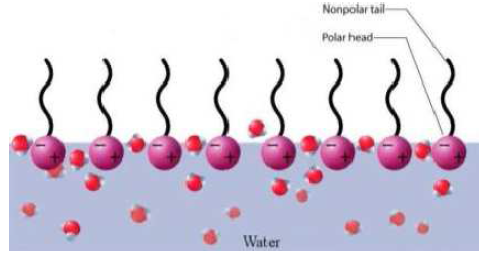
\includegraphics[width=0.5\linewidth]{images/chemical/molekul} 

}

\caption{Molekul Surfaktan}\label{fig:unnamed-chunk-53}
\end{figure}

~

Berdasarkan gugus hidrofiliknya, molekul surfaktan dibedakan ke dalam 4 kelompok (Rieger, 1985; Rosen, 2004), yaitu:

\begin{enumerate}
\def\labelenumi{\alph{enumi}.}
\tightlist
\item
  Surfaktan anionik
  Surfaktan anionik adalah molekul yang bermuatan negatif pada gugus hidrofilik atau aktif permukaan (\emph{surface-active}), seperti gugus sulfat atau sulfonat.

  ~
\item
  Surfaktan kationik
  Surfaktan kationik H adalah senyawa yang bermuatan positif pada gugus hidrofiliknya atau bagian aktif permukaan, seperti quarternery ammonium salt (QUAT).

  ~
\item
  Surfaktan non-ionik
  Surfaktan non-ionik adalah surfaktan yang tidak bermuatan atau tidak terjadi ionisasi molekul. Sifat hidrofilik disebabkan karena keberadaan gugus oksigen eter atau hidroksil.

  ~
\item
  Surfaktan amfoterik
  Surfaktan amfoterik adalah surfaktan yang bermuatan positif dan negatif pada molekulnya, dimana muatannya bergantung kepada pH. Pada pH rendah akan bermuatan negatif dan pada pH tinggi akan bermuatan positif. (Mathenson, 1996; Rosen, 2004).

  ~
\end{enumerate}

Dalam aplikasinya, keempat jenis surfaktan tersebut memiliki fungsi yang spesifik dan kondisi lingkungan kerja yang spesifik. Surfaktan anionik sangat baik digunakan untuk stimulasi batuan \emph{sandstone.} Adanya unsur silika di dalam batuan \emph{sandstone} yang bermuatan negatif akan menyebabkan \emph{water wet} pada formasi batuan \emph{sandstone.} Kondisi ini akan menyebabkan turunnya gaya adhesi antara minyak dan batuan sehingga minyak akan lepas dan lebih mudah mengalir dan sifat batuan akan berubah menjadi \emph{water wet}. Sebaliknya pada batuan \emph{limestone} yang bermuatan positif, penggunaan surfaktan anionik akan menyebabkan batuan bersifat \emph{oil wet} (Allen and Robert, 1993).

Surfaktan kationik dengan muatan gugus hidrofiliknya yang positif akan merubah \emph{wettability} batuan yang memiliki muatan positif menjadi water wet seperti batuan karbonat dan akan merubah \emph{wettability} batuan yang bermuatan negatif seperti batuan sandstone menjadi \emph{oil} \emph{wet.} Berbeda dengan surfaktan anionik dan kationik, surfaktan non-ionik yang tidak memiliki muatan pada gugus hidrofiliknya menyebabkannya \emph{compatible} pada kedua jenis batuan. Surfaktan nonionik akan menyebabkan water wet baik pada batuan karbonat maupun \emph{sandstone.} Sedangkan penggunaan surfaktan amfoterik pada kedua jenis batuan tersebut tergantung pada pH larutan dimana surfaktan tersebut bekerja. Pada kondisi pH \textgreater{} 7 (basa), gugus hidrofilik surfaktan amfoterik akan bermuatan positif sehingga akan menyebabkan \emph{water} \emph{wet} pada batuan yang memiliki muatan positif (karbonat). Pada pH \textless{} 7 (asam), gugus hidrofilik surfaktan amfoterik akan bermuatan negatif sehingga akan menyebabkan \emph{water} \emph{wet} pada batuan yang memiliki muatan negatif (\emph{sandstone}), sedangkan pada pH = 7, gugus hidrofilik surfaktan amfoterik tidak akan bermuatan. Namun pada aplikasi stimulasi surfaktan, surfaktan amfoterik digunakan terbatas sebagai pencegah korosi dan agen pembusa (Allen and Robert, 1993; Mulyadi, 2002).

Menurut Mathenson (1996), kelompok surfaktan yang penggunaannya dalam jumlah terbesar adalah surfaktan anionik. Karakteristiknya yang hidrofilik disebabkan karena adanya gugus ionik yang cukup besar, yang biasanya berupa grup sulfat atau sulfonat. Beberapa contoh surfaktan anionik, yaitu \emph{linear alkilbenzen sulfonat} (LAS), \emph{alcohol sulfat} (AS), \emph{alcohol eter sulfat} (AES), \emph{alfa olefin sulfonat} (AOS), paraffin (\emph{secondary alkane sulfonate}, SAS), dan \emph{metil ester sulfonat} (MES).

Mekanisme surfaktan dalam proses \emph{Enhanced Oil Recovery} adalah dengan cara menurunkan tegangan antarmuka, mengubah \emph{wettability}, bersifat sebagai \emph{emulsifier}, menurunkan viskositas dan menstabilkan dispersi sehingga memudahkan proses produksi. Untuk mendorong minyak yang terjebak dalam pori batuan, maka gaya kapilaritas dalam pori-pori harus diturunkan dengan cara menurunkan nilai IFT (\emph{Interfacial Tension}) dan menurunkan saturasi minyak. Surfaktan yang berada di dalam \emph{slug} harus dibuat agar membentuk \emph{micelle}, yaitu surfaktan yang aktif dan mampu mengikat air dan minyak pada konsentrasi tertentu. Jika konsentrasinya masih kecil,maka campuran surfaktan tersebut masih berupa monomer (belum aktif). Untuk itu, setiap slug perlu diketahui \emph{critical micelles concentration} (CMC), yaitu nilai konsentrasi tertentu dimana surfaktan yang semula monomer berubah menjadi \emph{micelles}. Hal yang penting dalam proses penggunaan surfaktan untuk menghasilkan \emph{recovery} minyak yang tinggi adalah (Pithapurwala, et al, 1986):

\begin{itemize}
\tightlist
\item
  Memiliki IFT yang sangat rendah (minimal 10-3 dyne/cm) antara \emph{chemical bank} dan \emph{residual oil}; dan antara \emph{chemical bank} dan \emph{drive fluid}.
\item
  Memiliki kecocokan dengan air formasi dan kestabilan terhadap temperatur.
\item
  Memiliki \emph{mobility control}.
\item
  Kelayakan ekonomis proses.
\end{itemize}

Proses injeksi surfaktan perlu memperhatikan besar bilangan kapiler terhadap penurunan saturasi minyak tersisa (\emph{S\textsubscript{or}}). Biasanya reservoir yang diinjeksi surfaktan memiliki harga saturasi minyak tersisa di bawah 45\% dengan nilai bilangan kapiler berkisar 10\textsuperscript{-4} - 10\textsuperscript{-2}, sehingga pendesakan surfaktan optimal. Semakin rendah saturasi minyak tersisa pada suatu reservoir, maka semakin besar bilangan kapiler yang dibutuhkan agar pendesakan surfaktan optimal (Lake, 1989). Untuk memperbesar bilangan kapiler diperlukan tegangan antarmuka yang rendah. Hubungan antara bilangan kapiler dengan tegangan antar muka adalah sebagai berikut.
\[N_{cap}=\mu \frac{\nu}{\sigma}...(1)\]
dimana N\textsubscript{c} adalah bilangan kapiler, \(\mu\) adalah viskositas fluida pendesak (cP), \(\nu\) adalah laju injeksi fluida pendesak, dan \(\sigma\) adalah tegangan antarmuka (dyne/cm).

Penurunan nilai tegangan antarmuka dapat dilakukan dengan menambahkan surfaktan. Surfaktan yang baik adalah mampu menurunkan nilai tegangan permukaan hingga \emph{ultra low} IFT yaitu lebih rendah dari 10\textsuperscript{-2} dyne/cm, karena pada kondisi tersebut maka bilangan kapiler akan semakin tinggi sehingga \emph{recovery factor} (RF) juga makin meningkat

\hypertarget{sifat-fisis-dan-mekanisme-kerja-alkali}{%
\subsection{Sifat Fisis dan Mekanisme Kerja Alkali}\label{sifat-fisis-dan-mekanisme-kerja-alkali}}

\emph{Alkaline flooding} (atau \emph{caustic flooding}) merupakan salah satu metode \emph{Enhanced Oil Recovery} (EOR) dimana dilakukan injeksi air dengan penambahan agen alkali pH tinggi (basa). Alkali memiliki kesamaan fungsi dengan injeksi surfaktan, namun memiliki cost yang lebih rendah dalam aplikasi penggunaannya.

Tingginya pH dicirikan dengan tingginya konsentrasi anion hidroksida (OH-). Jenis \emph{chemical} yang biasanya digunakan adalah Natrium Hidroksida (NaOH), Sodium Orthosilicate (NaSiO\textsubscript{6}), dan Natrium Carbonate (Na\textsubscript{2}CO\textsubscript{3}).

Dengan menginjeksikan alkali, diharapkan terjadi penurunan tegangan permukaan (IFT), gejala emulsi, dan perubahan \emph{wettability}. Berdasarkan jenis chemical yang digunakan, maka \emph{alkaline flooding} akan bekerja optimum bila digunakan pada viskositas fluida sedang, fluida dengan API \emph{gravity} rendah, dan karakteristik oil yang \emph{naphtenic}.

Tipe material alkali yang sering digunakan pada proyek-proyek EOR adalah sodium hydroxide dan sodium othosilicate. Bahan lain yang ditelah diteliti diantaranya juga sodium carbonate, ammonium hydroxide, polyphosphate, dan hydroxyl amine.

\emph{Alkaline flooding} memperbaiki \emph{recovery} dari \emph{acidic oils} dengan dua tahap proses (Castor, 1979). Tahap pertama melibatkan mobilisasi dari \emph{residual oil} dengan perubahan konfigurasi seperti emulsifikasi dan \emph{wettability alteration}. \emph{Surface-active salt} dibentuk secara \emph{in situ} dengan melibatkan reaksi asam-basa antara alkali dan \emph{organic acids} di dalam \emph{residual oil}. Surfaktan yang terbentuk memiliki sifat-sifat berikut:

\begin{enumerate}
\def\labelenumi{\arabic{enumi}.}
\tightlist
\item
  Mengadsorbsi pada \emph{oil-water interface} ke interfacial tension yang lebih rendah. Pada beberapa kasus hal tersebut menyebabkan \emph{spontaneous emulsification} dan \emph{phase swelling}.
\item
  Bereaksi atau \emph{adsorb} pada permukaan batuan, merubah karaketeristik \emph{wettability} batuan, dan konfigurasi dari \emph{residual ganglia crude oil} (Castor, 1979).
\end{enumerate}

Tahap kedua melibatkan modifikasi dari karakteristik produksi makroskopik dari fasa minyak yang bergerak. Efisiensi \emph{recovery} minyak secara keseluruhan dapat meningkat pada tahap ini dengan peningkatan \emph{displacement efficiency} melalui \emph{mobility control}.

Johnson (1976) me-\emph{review} mekanisme dimana \_alkaline floodin\_g dapat meningkatan perolehan minyak yang bersifat \emph{acidic} dari reservoir terdeplesi parsial:

\begin{enumerate}
\def\labelenumi{\arabic{enumi}.}
\tightlist
\item
  Emulsifikasi dan \emph{entrainment}
  Pada mekanisme ini (pertama dipublikasikan oleh Subkow, 1942), Subkow menyebutkan bahwa konsentrasi alkali dan pH harus dapat membuat emulsi \emph{oil-in-water} yang stabil terbentuk pada proses emulsifikasi dan \emph{entrainment}.

  ~
\item
  Emulsifikasi dan \emph{entrapment}
  Pada proses ini, minyak yang teremulsi kembali terjebak di dalam porous medium pada \emph{pore throats} yang terlalu kecil bagi \emph{droplet} emulsi untuk masuk mendorong air yang diinjeksi kedalam pori yang sebelumnya belum tersapu. Hasil dari penurunan pada \emph{mobility} dari fasa \emph{aqueous} dengan peningkatan \emph{displacement efficiency} dan penurunan jumlah \emph{viscous fingering} (Jennings, et.al., 1974).

  ~
\item
  Perubahan \emph{wettability} dari \emph{water-wet} ke \emph{oil-wet}
  \emph{Wettability} berubah karena reaksi antara \emph{caustic} dan \emph{acidic polar compounds} yang menempel pada batuan reservoir \emph{oil-wet}. Perubahan \emph{wettability} ini menghasilkan peningkatan pada \emph{oil/water relative permeability ratio} dan peningkatan pada \emph{displacement efficiency}.

  ~
\item
  Perubahan \emph{wettability} dari \emph{oil-wet} ke \emph{water-wet}
  Cooke et al.~(1974) merekomendasikan mekanisme ini dimana alterasi dari \emph{wettability} dari \emph{water-wet} ke \emph{oil-wet} menyebabkan fasa kontinu \emph{non-wetting residual oil} menyebar ke fasa \emph{wetting} kontinu. Secara simultan, \emph{interfacial tension} yang rendah mempengaruhi formasi dari emulsi \emph{alkali-in-oil} yang menyumbat jalur aliran dan juga mempengaruhi \emph{pressure gradient} yang tinggi disekitarnya. \emph{Pressure gradient} yang tinggi ini mengatasi gaya kapiler yang sudah menurun dan kemudian dapat menurunkan \emph{residual oil saturation}.

  ~

  5.Tambahan beberapa mekanisme diantaranya adalah penurunan \emph{interfacial tension} dan \emph{solubilization interfacial films}.

  ~
\end{enumerate}

Selain itu, Johnson juga mendiskusikan variasi dan kombinasi 4 dasar mekanisme:

\begin{enumerate}
\def\labelenumi{\alph{enumi}.}
\tightlist
\item
  \emph{Cyclic emulsification} dan \emph{entrapment process} (Sarem 1974).
\item
  \emph{Alternate emulsification-entrapment} dan \_emulsification entrainment proces\_s (Wade dan Lechtenberg, 1978).
\item
  \emph{Concurrent entrainment} dan \emph{entrapment seteleh emulsification}, \emph{wettability alteration}, dan \emph{chromatographic wettability reversal} (Radke dan Somerton, 1977, 1978; Castor et al., 1978).
\end{enumerate}

\hypertarget{mekanisme-proses-injeksi-kimia}{%
\section{Mekanisme Proses Injeksi Kimia}\label{mekanisme-proses-injeksi-kimia}}

Skema injeksi surfaktan-polimer dapat dilihat pada gambar berikut.

\textbackslash begin\{figure\}

\{\centering 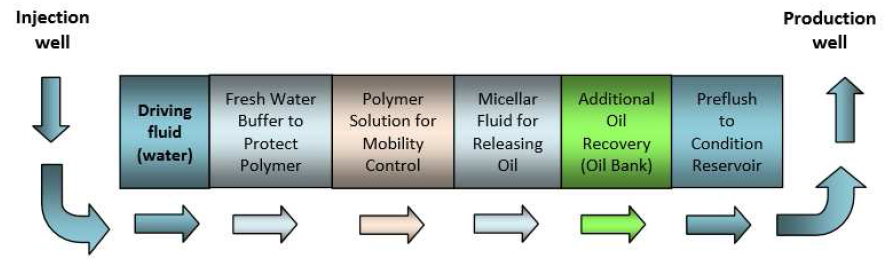
\includegraphics[width=0.5\linewidth]{images/chemical/skema}

\}

\textbackslash caption\{Skema injeksi \emph{micellar-polymer}\}\label{fig:unnamed-chunk-54}
\textbackslash end\{figure\}

~

Secara garis besar, injeksi surfakta-polimer terdiri dari:

\begin{itemize}
\tightlist
\item
  \textbf{Chase water}, digunakan sebagai pendorong fluida injeksi dari sumur injeksi ke sumur produksi
\item
  \textbf{Polimer \emph{slug}}, penggunaan polimer dalam injeksi surfaktan berfungsi sebagai \emph{mobility buffer},yaitu sebagai pengontrol mobilitas surfaktan dalam rangka effisiensi penyapuan dan melindungi surfaktan dari fluida pendorong. \emph{Mobility buffer} biasanya berupa campuran dari 250 -- 2500 gr/cm\textsuperscript{3} polimer, 0 - 1\% alkohol, \emph{stabilizers} dan \emph{biocide}, dimana volumenya berkisar antara 1 -- 100\% dari volume pori injeksi (V\textsubscript{pf}).
\item
  \textbf{\emph{Micellar} (Surfaktan) \emph{slug}}, berupa surfaktan dan tambahan \emph{oil recovering agent} yang berupa alkohol (0 - 5\%), cosurfactan (0 - 5\%), minyak, dan polimer. Volume larutan berkisar antara 5 -- 20\% V\textsubscript{pf}.
\item
  \textbf{Preflush}, merupakan larutan pembuka yang berupa air garam (Na\textsuperscript{+}, Ca\textsuperscript{2+}) yang berfungsi untuk menurunkan salinitas air formasi, sehingga memungkinkan terjadinya percampuran antara air formasi dengan surfaktan yang diinjeksikan. Volume dari preflush berkisar antara 0 -- 100\% V\textsubscript{pf}.
\end{itemize}

Larutan surfaktan yang diinjeksikan ke dalam reservoir akan bersinggungan dengan permukaaan gelembung minyak, surfaktan bekerja sebagai zat aktif permukaan untuk menurunkan tegangan permukaan minyak-

Slug polimer yang diinjeksikan diantara slug fresh water adalah untuk mengurangi kontak langsung dengan air reservoir yang mengandung garam. Air garam menurunkan viskositas polimer. Jadi injeksi polimer tidak menurunkan saturasi minyak sisa, tetapi memperbaiki perolehan minyak yang lebih dari injeksi air denan menaikkan volume reservoir yang berhubungan.

\hypertarget{asumsi-dan-batasan-dalam-predictive-model}{%
\section{\texorpdfstring{Asumsi dan Batasan Dalam \emph{Predictive Model}}{Asumsi dan Batasan Dalam Predictive Model}}\label{asumsi-dan-batasan-dalam-predictive-model}}

Beberapa asumsi dan batasan dalam \emph{predictive model} yang dibangun diantaranya adalah sebagai berikut:

\begin{enumerate}
\def\labelenumi{\arabic{enumi}.}
\tightlist
\item
  \emph{Predictive model} dibangun hanya untuk litologi \emph{sandstone}.
\item
  \emph{Micellar-polymer} (MP) flood diasumsikan dilakukan setelah \emph{waterflood}.
\item
  Temperatur formasi maksimum dibatasi sebesar 230°F, dan salinitas air formasi maksimum dibatasi sebesar 80000 ppm TDS.
\item
  \emph{Target oil} dari MP \emph{flood} adalah \emph{residual oil} di zona yang sebelumnya telah disapu oleh air saat \emph{waterflood}. Fraksi target oil yang dapat diproduksikan didefinisikan sebagai efisiensi perolehan (\emph{overall recovery efficiency} (\emph{E\textsubscript{R}})). \emph{E\textsubscript{R}} dinyatakan sebagai fungsi dari bilangan kapiler, \emph{vertical sweep efficiency}, dan \emph{mobility buffer efficiency}.
\item
  \emph{Areal sweep} dari MP \emph{flood} diasumsikan sama dengan \emph{areal sweep} dari \emph{waterflood} yang telah dilakukan sebelumnya.
\item
  Dalam algoritma \emph{predictive model}, adsorpsi surfaktan ditinjau, namun adsorpsi polimer diabaikan.
\item
  \emph{Displacement efficiency} dari MP \emph{flood} merupakan fungsi dari bilangan kapiler, dimana bilangan kapiler merupakan fungsi dari permeabilitas, \emph{depth}, dan \emph{well spacing}.
\item
  \emph{Interfacial tension} antara \emph{micellar}-minyak dianggap konstan pada nilai 10\textsuperscript{-3} dyne/cm.
\item
  \emph{Predictive model} hanya berlaku untuk pola \emph{five-spot}.
\item
  Laju injeksi diasumsikan konstan sepanjang periode \emph{flooding}.
\item
  Dalam menghitung \emph{injectivity}, viskositas surfaktan diasumsikan sama dengan viskositas minyak.
\item
  Profil produksi minyak dari MP \emph{flood} untuk reservoir heterogen diasumsikan berbentuk segitiga. Luas daerah di bawah kurva produksi minyak, yang merupakan kumulatif produksi minyak, digunakan untuk mengestimasi nilai \emph{peak oil rate}.
\item
  \emph{Breakthrough} minyak dan surfaktan dihitung dari teori \emph{fractional flow}.
\item
  Laju produksi minyak maksimum diasumsikan terjadi saat periode \emph{surfactant breakthrough}.
\item
  Tidak terjadi perubahan kecepatan pada \emph{surfactant front} saat \emph{polymer front} mendahului \emph{surfactant front}.
\item
  Dalam menghitung \emph{vertical sweep efficiency}, diasumsikan beberapa hal berikut:

  \begin{itemize}
  \tightlist
  \item
    Saturasi minyak \emph{movable} di reservoir terdistribusi secara \emph{uniform}.
  \item
    Adanya \emph{lag} dari \emph{surfactant front} yang disebabkan oleh adsorpsi surfaktan terjadi secara \emph{uniform} sepanjang reservoir.
  \item
    Dispersi dari \emph{slug} surfaktan diabaikan.
  \item
    Nilai \emph{mobility ratio} di setiap \emph{front bank} di reservoir adalah satu.
  \item
    Di zona yang telah tersapu oleh surfaktan, nilai saturasi minyak berkurang menjadi suatu nilai konstan yang bersesuaian dengan kurva \emph{capillary desaturation}.
  \end{itemize}
\end{enumerate}

\hypertarget{konsep-dan-algoritma-yang-digunakan-dalam-predictive-model}{%
\section{\texorpdfstring{Konsep dan Algoritma yang Digunakan Dalam \emph{Predictive Model}}{Konsep dan Algoritma yang Digunakan Dalam Predictive Model}}\label{konsep-dan-algoritma-yang-digunakan-dalam-predictive-model}}

\hypertarget{perhitungan-target-oil}{%
\subsection{\texorpdfstring{Perhitungan \emph{Target Oil}}{Perhitungan Target Oil}}\label{perhitungan-target-oil}}

\emph{Target oil} dari MP \emph{flood} adalah \emph{residual oil} yang berada di zona yang telah tersapu oleh air pada proses \emph{waterflood} yang telah diterapkan sebelum MP \emph{flood.} Maksud dari pernyataan ini adalah \emph{areal} \emph{sweep} \emph{efficiency} dari MP \emph{flood} dianggap sama dengan \emph{areal} \emph{sweep} \emph{efficiency} pada \emph{waterflood} (\emph{areal} \emph{sweep} \emph{efficiency} tidak berubah). Karena \emph{target} \emph{oil} hanya berada di zona sapuan sebelumnya, maka minyak yang berada di luar zona sapuan tidak dianggap sebagai \emph{target} \emph{oil.} Nilai \emph{target} \emph{oil} dinyatakan oleh persamaan berikut.
\[TO = \left[ \frac{S_{orw}}{S_{oi}-S_{orw}} \right] \left[N_p-OOIP \left( 1- \frac{B_{oi}}{B_{of}}\right) \right] \left[ 1-f_{bw}-f_{gc} \right]...(2)\]
dimana:
\(f_{bw}\) = zona reservoir \emph{unswept} di atas \emph{bottom water}
\(f_{gc}\) = zona reservoir \emph{unswept} di bawah \emph{gas cap}

Maka, \emph{floodable pore volume} dinyatakan oleh persamaan berikut.
\[V_p = TO \left( \frac{B_{of}}{S_{orw}}\right)...(3)\]
Jika nilai TO tidak dapat diperoleh dari persamaan (2) karena terdapat parameter yang nilainya tidak diketahui, maka nilai TO dapat diapproksimasi menggunakan persamaan (3) dengan nilai \emph{V\textsubscript{p}} diasumsikan sama dengan \(A\phi h\).

\hypertarget{laju-alir-dan-bilangan-kapiler}{%
\section{Laju Alir dan Bilangan Kapiler}\label{laju-alir-dan-bilangan-kapiler}}

Persamaan laju alir dan bilangan kapiler diturunkan dari persamaan aliran \emph{steady-state} Muskat, dimana Muskat mendefinisikan \emph{injectivity coefficient}, \emph{C\textsubscript{p}}, sebagai:
\[\frac{C_pD}{\mu_o} \equiv \frac{\Delta P}{\mu}...(4) \]
Persamaan laju alir (dalam satuan bbl/day) adalah:
\[q = \frac{0.003541C_pkhD}{\mu_o \left[ 5.58+ \frac{1}{2}\ln A\right]}...(5)\]
dimana \emph{A} adalah luas daerah untuk setiap pola injeksi.
Dari definisi bilangan kapiler,
\[N_{cap}=u \frac{\mu}{\sigma}...(6)\]
Laju alir fluida (dalam satuan ft/day) untuk pola \emph{5-spot} dinyatakan oleh Parsons sebagai:
\[u = \frac{0.000055C_pkD}{\mu_o \sqrt A \left[ 5.58+ \frac{1}{2}\ln A\right]}...(7)\]
Dengan mengasumsikan \(\mu\) ≅ \(\mu_o\) dan \(\sigma\) = 10\textsuperscript{-3} dyne/cm pada persamaan (6), maka substitusi persamaan (6) ke persamaan (7) memberikan persamaan bilangan kapiler berikut.
\[N_{cap} = \frac{(1.9 \times 10^{-7})C_pkD}{\sqrt A \left() 5.58+ \frac{1}{2}\ln A\right)}...(8)\]
Dapat dilihat pada persamaan (5) dan (8) bahwa nilai laju alir dan bilangan kapiler sangat dipengaruhi oleh parameter \emph{injectivity coefficient}, \emph{C\textsubscript{p}}.

\hypertarget{surfactant-retention-pada-batuan-sandstone}{%
\subsection{\texorpdfstring{\emph{Surfactant Retention} Pada Batuan \emph{Sandstone}}{Surfactant Retention Pada Batuan Sandstone}}\label{surfactant-retention-pada-batuan-sandstone}}

Mekanisme \emph{surfactant retention} ditinjau hanya disebabkan oleh adsorpsi pada \emph{clay} yang terdapat di dalam \emph{sandstone}, sehingga besarnya \emph{surfactant retention} dipengaruhi oleh fraksi berat \emph{clay}. \emph{Surfactant retention} dinyatakan dalam satuan \emph{pore volume} injeksi surfaktan \emph{slug} adalah:
\[D_s = \left(\frac{1-\phi}{\phi} \right) \left( \frac{\rho_sa_s}{\rho_sC_s}\right)\frac {1}{1000}...(9)\]
dimana:
\(a_s\) = \emph{surfactant retention} dalam satuan mg surfaktan/g batuan
\(C_s\) = fraksi volume surfaktan di dalam \emph{slug}

Nilai \emph{surfactant retention}, \(a_s\), umumnya diperoleh melalui eksperimen di laboratorium. Jika tidak terdapat data laboratorium, maka \(a_s\) dapat diestimasi dari korelasi antara adsorpsi surfaktan pada \emph{sandstone} dengan total fraksi \emph{clay} dalam \emph{sandstone} seperti diperlihatkan pada grafik berikut.

\textbackslash begin\{figure\}

\{\centering \includegraphics[width=0.5\linewidth]{images/chemical/adsorpsi}

\}

\textbackslash caption\{Korelasi grafik antara adsorpsi surfaktan dengan total fraksi berat \emph{clay} dalam \emph{sandstone}\}\label{fig:unnamed-chunk-55}
\textbackslash end\{figure\}

~

Selain melalui korelasi grafik di atas, persamaan berikut, yang menyatakan \_surfactant retentio\_n sebagai fungsi dari fraksi berat \emph{clay}, juga dapat digunakan untuk mengestimasi nilai \(a_s\) jika nilai fraksi berat \emph{clay} diketahui.
\[a_s = 3.3 \times wt.fr.clay ... (10)\]
Jika fraksi berat clay juga tidak diketahui, maka nilai \(a_s\) = 0.4 \emph{mg/g} dapat digunakan sebagai nilai \emph{default} untuk \emph{surfactant retention}.

\hypertarget{perhitungan-oil-recovery}{%
\subsection{\texorpdfstring{Perhitungan \emph{Oil Recovery}}{Perhitungan Oil Recovery}}\label{perhitungan-oil-recovery}}

Efisiensi perolehan minyak (\emph{oil recovery efficiency}) tanpa menyertakan pengaruh \emph{crossflow} dinyatakan oleh persamaan berikut.
\[E_r^0=E_DE_VE_{MB}...(11)\]
dimana \emph{E\textsubscript{D}} menyatakan \emph{displacement efficiency}, \emph{E\textsubscript{V}} menyatakan \emph{vertical sweep efficiency}, dan \emph{E\textsubscript{MB}} menyatakan \emph{mobility buffer} (polimer) \emph{sweep efficiency}.

\emph{Displacement efficiency} didefinisikan sebagai berikut.
\[E_D = \frac{(S_{orw})-(S_{orc}}{(S_{orw}}...(12)\]
dimana:
\(S_{orc}\) = nilai saturasi minyak di zona sapuan \emph{micellar slug}.

\emph{Displacement efficiency} merupakan fungsi dari bilangan kapiler yang terhubung melalui kurva \emph{capillary desaturation}. Terdapat tiga cara untuk menentukan nilai \emph{displacement efficiency}.

\begin{enumerate}
\def\labelenumi{\alph{enumi}.}
\tightlist
\item
  Tentukan nilai bilangan kapiler, \emph{N\textsubscript{cap}}, dari persamaan (8), kemudian gunakan kurva \emph{capillary desaturation} yang khusus dibangun untuk reservoir target.
\item
  Nilai \emph{displacement efficiency} diperoleh secara langsung dari hasil analisis core di laboratorium dengan nilai \(\frac{V_{ps}}{D_s}\) yang tinggi.
\item
  Nilai bilangan kapiler ditentukan dari persamaan (8), kemudian digunakan kurva \emph{capillary desaturation} untuk Berea \emph{rock} yang dibangun oleh Gupta-Trushenski. Gambar berikut memperlihatkan kurva ini.
\end{enumerate}

\textbackslash begin\{figure\}

\{\centering \includegraphics[width=0.5\linewidth]{images/chemical/berea}

\}

\textbackslash caption\{Kurva \emph{capillary desaturation} untuk Berea \emph{rock} yang disusun oleh Gupta dan Trushenki\}\label{fig:unnamed-chunk-56}
\textbackslash end\{figure\}

~

Pengaruh \emph{wettability} terhadap \emph{displacement efficiency} diwakili oleh rasio antara nilai \emph{end-point} permeabilitas relatif air terhadap minyak, yaitu:
\[R = \frac{k_{rw}^0}{k_{ro}^0}...(13)\]
Nilai R =0.2 menandakan sistem \emph{water wet}, sedangkan nilai R = 10 menandakan sistem \emph{oil wet}.

\emph{Vertical sweep efficiency} dinyatakan sebagai fungsi dari keheterogenan reservoir, yang diwakili oleh koefisien variasi permeabilitas Dykstra-Parsons (\emph{V\textsubscript{DP}}) dan rasio \(\frac{V_{ps}}{D_s}\), \emph{Vertical sweep efficiency} secara matematis dinyatakan oleh persamaan berikut.
\[E_V = C_m + \frac{V_{ps}}{D_s}(1-F_m)...(14)\]
dimana \(\frac{V_{ps}}{D_s}\) adalah \emph{dimensionless surfactant slug size}, yaitu rasio antara nilai \emph{pore volume slug} injeksi surfaktan yang sebenarnya (\emph{V\textsubscript{PS}}) terhadap nilai \emph{pore volume surfactant retention} (\emph{D\textsubscript{S}}).

Pada persamaan (14), \emph{C\textsubscript{M}} dan \emph{F\textsubscript{M}} menyatakan \emph{storage capacity} dan \emph{flow capacity} dari lapisan M, yaitu lapisan dimana polimer \emph{front} mendahului \emph{surfaktan front}. Nilai \emph{F\textsubscript{M}} dihitung menggunakan persamaan berikut.

Jika \(\frac{V_{ps}}{D_s} \leq EFF,\)
\[F_M = \frac{\left( \frac{EFF}{\frac{V_{ps}}{D_s}}\right)^{0.5}-EFF}{1-EFF}...(15)\]
Jika \(\frac{V_{ps}}{D_s} > EFF,\)
\[F_M = 1...(16)\]
Sedangkan nilai \emph{C\textsubscript{M}} dihitung menggunakan persamaan berikut.
\[C_M = \frac{1}{EFF \left( \frac{1}F_M-1{}\right)+1}...(17)\]
Parameter EFF menyatakan \emph{effective mobility ratio}, yang dihitung sebagai fungsi dari koefisien variasi permeabilitas Dykstra-Parsons (\emph{V\textsubscript{DP}}).
\[EFF = 10^{ \left( \frac{V_{DP}}{(1-V_{DP})^{0.2}} \right)}...(18)\]
Untuk lapisan 1-D homogen, \(F_M = C_M = 0\), dan \(E_V = 1\).

\emph{Mobility buffer sweep efficiency} (\emph{E\textsubscript{MB}}) didefinisikan sebagai rasio antara volume produksi minyak terhadap volume minyak mobile di reservoir. \emph{E\textsubscript{MB}} merupakan fungsi dari \emph{pore volume} injeksi polimer (\emph{V\textsubscript{MB}}), koefisien variasi permeabilitas Dykstra-Parsons (\emph{V\textsubscript{DP}}), dan rasio \(\frac{V_{ps}}{D_s}\). \emph{Mobility buffer sweep efficiency} dinyatakan oleh persamaan berikut.
\[E_{MB}=(1-E_{MBo}) \left[ 1-exp \left( \frac{- \alpha V_{MB} }{E_V^{\beta}} \right) \right]+E_{MBo}...(19)\]
dimana:
\[E_{MBo} = E_{MB|V_{MB}=0}...(20)\]
Nilai dan korelasi mengenai parameter-parameter \(\alpha\), \(\beta\), dan \emph{E\textsubscript{MBo}} diperoleh dari hasil studi simulasi. Hasil simulasi memberikan nilai-nilai berikut sebagai nilai yang sesuai untuk digunakan pada persamaan (19).
\[\alpha = 0.4\]
\[\beta = 1.2\]
\[E_{MBo} = 0.71 - 0.6V_{DP}...(21)\]
Maka, perolehan volume minyak target dinyatakan oleh persamaan berikut.
\[N_{TO} = E_R^0(TO)...(22)\]
\#\#\# Karakteristik Produksi Minyak dan Koreksi Terhadap \emph{Crossflow}

Berdasarkan teori \_fractional flo\_w, \emph{micellar-polymer flood} akan membentuk \emph{oil bank} di reservoir dengan nilai saturasi minyak \emph{S\textsubscript{ob}} dan fraksi aliran minyak \emph{f\textsubscript{ob}}. Di belakang oil bank adalah \emph{surfactant bank}, dimana \emph{surfactant front} bergerak dengan kecepatan yang dinyatakan oleh:
\[v_s = \frac{1}{1+D_s-S_{orc}}...(23)\]
Kecepatan \emph{surfactant front}, persamaan (23), dapat pula dinyatakan dalam bentuk lain, yaitu menggunakan nilai saturasi minyak dan fraksi aliran minyak di \emph{oil bank}, \emph{S\textsubscript{ob}} dan \emph{f\textsubscript{ob}}.
\[v_s=\frac{f_{ob}}{S_{ob}-S_{orc}}=\frac{1-f_{wb}}{1-S_{wb}-S_{orc}}...(24)\]
Nilai \emph{S\textsubscript{wb}} dan \emph{f\textsubscript{wb}} diperoleh dari analisis kurva \emph{fractional flow}. Tinjau kurva \emph{fractional flow} air dan minyak, dimana selain kurva \emph{fractional flow}, terdapat pula garis lurus yang berawal di titik (\emph{f\textsubscript{w}} = 0, \emph{S\textsubscript{w}} = -\emph{D\textsubscript{s}}) dan berakhir di titik (\emph{f\textsubscript{w}} = 1, \emph{S\textsubscript{w}} = 1 - \emph{S\textsubscript{orc}}). Garis lurus ini akan berpotongan dengan kurva \emph{fractional flow} di titik (\emph{S\textsubscript{wb}},\emph{f\textsubscript{wb}}). Gambar di halaman selanjutnya memperlihatkan penjelasan

Maka, nilai saturasi air dan fraksi aliran air \emph{di oil bank},\emph{S\textsubscript{wb}} dan \emph{f\textsubscript{wb}} diperoleh dengan menentukan titik potong garis lurus terhadap kurva \emph{fractional flow}. Setelah kedua nilai parameter ini diperoleh, maka kecepatan \emph{surfactant front} yang dinyatakan oleh persamaan (24) dapat dihitung. Selanjutnya, kecepatan front \emph{oil bank} dihitung menggunakan persamaan berikut.
\[v_{ob} = \frac{f_{ob}-f_{oi}}{S_{ob}-S_{oi}}...(25)\]
dimana untuk perolehan tersier, \emph{S\textsubscript{oi}} = \emph{S\textsubscript{or}} dan \emph{f\textsubscript{oi}} = 0.

\textbackslash begin\{figure\}

\{\centering \includegraphics[width=0.5\linewidth]{images/chemical/fractional}

\}

\textbackslash caption\{Kurva \emph{fractional flow} air, titik potong antara kurva \emph{fractional flow} dengan garis lurus memberikan nilai (\emph{S\textsubscript{wb}},\emph{f\textsubscript{wb}})\}\label{fig:unnamed-chunk-57}
\textbackslash end\{figure\}

~

Dari persamaan kecepatan \emph{surfactant front} dan \emph{oil bank front}, \emph{dimensionless breakthrough time} untuk \emph{oil bank} (\emph{t\textsubscript{Dob}}) dan \emph{surfactant bank} (\emph{t\textsubscript{Ds}}) untuk reservoir homogen dinyatakan oleh persamaan berikut.
\[t_{Dob}=\frac{1}{v_{ob}}...(26)\]
\[t_{Ds}=\frac{1}{v_{s}}...(27)\]
Untuk reservoir homogen, fungsi produksi \emph{dimensionless} dinyatakan sebagai berikut.

Untuk \(t_{D} \leq t_{Dob},\ oil\ cut = f_{oi}\)\\

Untuk \(t_{Dob} \leq t_{D} \leq t_{Ds},\ oil\ cut = f_{oc}\)

Untuk \(t_{D} > t_{Ds},\ oil\ cut = 0\)

Gambar berikut memperlihatkan kurva \emph{oil cut} terhadap waktu \emph{dimensionless}, \emph{t\textsubscript{D}}.

\textbackslash begin\{figure\}

\{\centering \includegraphics[width=0.5\linewidth]{images/chemical/octd}

\}

\textbackslash caption\{\emph{Oil cut} vs.~waktu \emph{dimensionless} untuk reservoir homogen\}\label{fig:unnamed-chunk-58}
\textbackslash end\{figure\}

~

Penjelasan karakteristik produksi di atas berlaku untuk reservoir homogen. Untuk reservoir heterogen, penjelasan karakteristik produksi dilakukan menggunakan koreksi terhadap parameter-parameter produksi homogen yang telah dijelaskan sebelumnya. Koreksi dilakukan terhadap faktor \emph{layering}. Untuk melakukan hal ini, profil produksi minyak diasumsikan berbentuk segitiga, yang dikarakterisasi oleh empat parameter berikut: \emph{oil breakthrough time} (\emph{t\textsubscript{ob}}), \emph{surfactant breakthrough time} (\emph{t\textsubscript{s}}), \emph{peak oil rate} (\emph{q\textsubscript{opk}}), dan \emph{time of zero rate} (\emph{t\textsubscript{sw}}).

\begin{figure}

{\centering \includegraphics[width=0.5\linewidth]{images/chemical/profilprod} 

}

\caption{Profil produksi minyak (diasumsikan berbentuk segitiga) untuk reservoir heterogen}\label{fig:unnamed-chunk-59}
\end{figure}

~

Analisis terhadap keempat parameter di atas akan dimulai dengan mendefinisikan parameter \_dimensionles\_s-nya. Waktu \_breakthrough \_minyak \emph{dimensionless} (\emph{t\textsubscript{Dob}}) dan waktu \_breakthroug\_h surfaktan \emph{dimensionless} (\emph{t\textsubscript{Ds}}) dinyatakan oleh dua persamaan berikut.
\[t_{Dob}=\frac{1}{(v_{ob})(EFF)}...(28)\]
\[t_{Ds}=\frac{1}{(v_{s})(EFF)}...(29)\]
Nilai fraksi aliran minyak tertinggi (\emph{peak oil fractional flow}) dinyatakan oleh:
\[f_{opk}=(f_{ob})(f_{fprim})...(30)\]
dengan
\[f_{fprim}=\frac{(EFF)(CFPRIM)}{[(EFF)(CFPRIM)]+1-CFPRIM}...(31)\]
\[CFPRIM=\frac{\left[\frac{1}{\left(\frac{v_{s}}{v_{ob}}\right)}\right]^{0.5}-1}{EFF-1}...(32)\]
Waktu \emph{dimensionless} saat laju alir minyak nol (\emph{time of zero oil rate dimensionless}), \emph{t\textsubscript{Dsw}}, dinyatakan oleh persamaan berikut.
\[t_{Dsw}=t_{Dob}+ \frac{2(E_R^0)(S_{orw})}{f_{opk}}...(33)\]
Pembahasan di atas memberikan nilai dari parameter-parameter dimensionless pada kurva laju produksi minyak, yaitu waktu \emph{dimensionless oil breakthrough} (\emph{t\textsubscript{Dob}}), waktu \emph{dimensionless} surfaktan \emph{breakthrough} (\emph{t\textsubscript{Ds}}), dan waktu \emph{dimensionless zero oil rate} (\emph{t\textsubscript{Dsw}}). Parameter-parameter \emph{dimensionless} ini selanjutnya akan dikonversi ke dalam nilai sebenarnya.

Untuk mengkonversi parameter dimensionless ke dalam nilai sebenarnya, dibutuhkan informasi mengenai laju alir fluida di reservoir. Nilai laju alir fluida reservoir pada kondisi aliran \emph{steady-state} dinyatakan oleh persamaan (5), yaitu:
\[q=\frac{0.003541C_pkhD}{\mu_o \left[ 5.58+ \frac{1}{2}\ln A\right]}\]
Setelah nilai laju alir fluida di reservoir diketahui, parameter-parameter \emph{dimensionless} pada persamaan (28), (29), dan (33) dapat dikonversi ke dalam nilai sebenarnya melalui persamaan-persamaan berikut.
\[t_{ob}=t_{Dob} \frac{(V_p)_{pat}}{q}...(34)\]
\[t_{s}=t_{Ds} \frac{(V_p)_{pat}}{q}...(35)\]
\[t_{sw}=t_{Dsw} \frac{(V_p)_{pat}}{q}...(36)\]
dimana:
\((V_p)_{pat}\) = \emph{pattern floodable pore volume}

Laju alir minyak tertinggi (\emph{peak oil rate}) terjadi saat waktu surfaktan \emph{breakthrough} (\emph{t\textsubscript{s}}). Nilai \emph{peak oil rate} dinyatakan oleh:
\[q_{opk} =q \frac{f_{opk}}{B_{of}}...(37)\]
Setelah nilai dari parameter-parameter kurva laju produksi minyak diketahui, volume produksi minyak dan produksi air untuk setiap periode dapat dihitung. Perhitungan volume produksi fluida dibedakan dalam tiga interval waktu, yaitu (1) produksi sebelum \emph{oil breakthrough} (\emph{t} \textless{} \emph{t\textsubscript{ob}}) dan setelah \emph{zero oil rate} (\emph{t} \textgreater{} \emph{t\textsubscript{sw}}), (2) produksi saat \emph{t\textsubscript{ob}} ≤ \emph{t} \textless{} \emph{t\textsubscript{s}}, dan (3) produksi saat \emph{t\textsubscript{s}} \textless{} \emph{t} ≤ \emph{t\textsubscript{sw}}.

Selama periode \emph{t\textsubscript{ob}} ≤ \emph{t} \textless{} \emph{t\textsubscript{s}}, nilai \emph{oil cut} akan terus naik secara linier karena semakin banyak lapisan yang memproduksikan minyak. Hal ini terjadi sampai tercapainya \emph{peak oil rate}, yaitu saat \emph{t} = \emph{t\textsubscript{s}}. Untuk periode \emph{t\textsubscript{s}} \textless{} \emph{t} ≤ \emph{t\textsubscript{sw}}, \emph{oil cut} akan terus menurun secara linier karena semakin banyak lapisan yang memproduksi surfaktan atau polimer. Kecepatan surfaktan \emph{front} diasumsikan tidak berubah selama mengalir di reservoir, juga saat \emph{polimer front} mendahului surfaktan \emph{front} di lapisan dengan nilai permeabilitas yang rendah.

Laju produksi minyak dan air untuk setiap periode dan setiap time step i adalah sebagai berikut. Untuk periode waktu pertama, yaitu \emph{t} \textless{} \emph{t\textsubscript{ob}} dan \emph{t} \textgreater{} \emph{t\textsubscript{sw}}:
\[q_o=0...(38)\]
\[q_w=q...(39)\]
Untuk periode waktu kedua, yaitu \emph{t\textsubscript{ob}} ≤ \emph{t} \textless{} \emph{t\textsubscript{s}}:
\[q_o(i)=q_{opk} \left( \frac{t(i)-t_{ob}}{t_s-t_{ob}} \right)...(40)\]
\[q_w(i)=\frac{q-[q_o(i)B_{of}]}{B_{wf}}...(41)\]
Untuk periode waktu kedua, yaitu \emph{t\textsubscript{s}} \textless{} \emph{t} ≤ \emph{t\textsubscript{sw}}:
\[q_o(i)=q_{opk} \left( \frac{t_{sw}-t(i)}{t_{sw}-t_s} \right)...(42)\]
\[q_w(i)=\frac{q-[q_o(i)B_{of}]}{B_{wf}}...(43)\]
Saat \emph{t(i)} = \emph{t\textsubscript{s}}, \emph{q\textsubscript{o}(i)} = \emph{q\textsubscript{opk}}.

Selanjutnya, nilai \emph{overall oil recovery efficiency} (\(E_R^0\)) akan dikoreksi terhadap efek \emph{crossflow}. Koreksi terhadap nilai \(E_R^0\) memberikan nilai \emph{corrected overall oil recovery efficiency} (\(E_R^C\)) seperti dinyatakan dalam persamaan berikut.
\[E_R^C= 0.04 \log (RL) + 0.064+E_R^0...(44)\]
\[RL = \sqrt \frac{k_v}{k_h} \left( \frac{XLIP}{h_{pay}} \right)...(45)\]
\[XLIP = 0.7071 \sqrt {43560(A_{pat})}...(46)\]
dimana:
\(APAT\) = \emph{pattern area}
\(h_{pay}\) = reservoir \emph{net pay}
\(RL\) = bilangan \emph{crossflow dimensionless}.

Rasio antara \emph{corrected overall oil recovery} dengan \emph{overall oil recovery} dinyatakan oleh parameter \emph{crossflow performance factor} (\emph{f\textsubscript{CF}}), yang didefinisikan oleh persamaan berikut.
\[f_{CF} = \frac{E_R^C}{E_R^0}...(47)\]

\hypertarget{karakteristik-injeksi-kimia}{%
\subsection{Karakteristik Injeksi Kimia}\label{karakteristik-injeksi-kimia}}

Terdapat dua zat kimia yang digunakan dalam \emph{micellar-polymer flooding}, yaitu surfaktan dan polimer. Volume injeksi \emph{slug} surfaktan per pola injeksi adalah:
\[BSL = (V_p)_{pat}V_{PS}...(48)\]
dimana \emph{V\textsubscript{PS}} adalah \emph{slug size} surfaktan injeksi. Adapun lama injeksi surfaktan dinyatakan oleh:
\[t_{surf} = \frac{\left( \frac{BSL}{q} \right)}{365}...(49)\]
Di lain pihak, volume injeksi polimer dinyatakan sebagai fungsi dari \emph{mobility rati} dan
\emph{wettability} dimana \emph{wettability} dinyatakan dalam bentuk rasio permeabilitas relatif \emph{end-point}, \(R=\frac{k_{rw}^0}{k_{ro}^0}\). Konsentrasi polimer awal dalam \emph{slug} polimer injeksi dinyatakan oleh persamaan berikut.
\[C_{poly}=111 \left( \frac{\mu_o}{\mu_w} \right)+B ...(50)\]
dimana:
Untuk \emph{R} \(leq\) 0.1,
\[B = 338...(51)\]
Untuk 0.1 \textless{} \emph{R} \textless{} 10,
\[B = 338 + \left[ (R-0.1) \left( \frac{1032}{9.9} \right)\right]...(52)\]
Untuk \emph{R} \(\geq\) 10,
\[B = 1370 ...(53)\]
Volume injksi \emph{slug}
polimer per pola injeksi dinyatakan oleh persamaan berikut.
\[BMB = (V_p)_{pat}V_{MB}...(54)\]
Sedangkan lama periode injeksi polimer dinyatakan oleh:
\[t_{MB}= \frac{\left( \frac{BMB}{q} \right)}{365}...(55)\]

\#\#\# Modifikasi \emph{Predictive Model} Untuk \emph{Caustic} dan \emph{Caustic-Polymer Flood}

Selain \emph{micellar-polymer}, pada predictive model yang dibangun terdapat juga pilihan tipe injeksi kimia lainnya, yaitu \emph{caustic flood}, \emph{caustic-polymer flood}, dan \emph{advanced caustic flood} (\emph{surfactant flood}). Untuk tiga tipe pilihan injeksi kimia ini, model melakukan modifikasi terhadap beberapa nilai parameter yang digunakan dalam algoritma \emph{micellar-polymer flood}. Tabel berikut merangkum modifikasi yang dilakukan.

\textbackslash begin\{figure\}

\{\centering \includegraphics[width=0.5\linewidth]{images/chemical/modifikasi}

\}

\textbackslash caption\{Modifikasi nilai sejumlah parameter MP \emph{flood} untuk kasus \emph{caustic} dan \emph{caustic-polymer flood}\}\label{fig:unnamed-chunk-60}
\textbackslash end\{figure\}

~

\hypertarget{persamaan-persamaan-dasar-dan-nilai-default-yang-digunakan-dalam-model}{%
\section{\texorpdfstring{Persamaan-Persamaan Dasar dan Nilai \emph{Default} yang Digunakan Dalam Model}{Persamaan-Persamaan Dasar dan Nilai Default yang Digunakan Dalam Model}}\label{persamaan-persamaan-dasar-dan-nilai-default-yang-digunakan-dalam-model}}

\hypertarget{viskositas-minyak-1}{%
\subsection{Viskositas Minyak}\label{viskositas-minyak-1}}

Viskositas minyak, \(\mu_o\), dihitung menggunakan korelasi Beggs-Robinson. Korelasi terlebih dahulu menghitung nilai viskositas \emph{dead oil}, \(\mu_{od}\).
\[\mu_{od}=10^x-1...(56)\]
dengan
\[X=\frac{Y}{T^{1.163}}\]
\[Y = 10^Z\]
\[Z= 3.0324-0.02023(API)\]
dimana:
\emph{T} = temperatur reservoir, \(\circ\)F
\emph{API} = \emph{gravity} minyak, \(\circ\)API.
Selanjutnya viskositas \emph{live oil} dihitung dengan persamaan berikut.
\[\mu_o = A (\mu_{od})^B...(57)\]
dengan
\[A=\frac{10.715}{(_s+100)^{0.515}}\]
\[B=\frac{5.44}{(_s+150)^{0.338}}\]

\hypertarget{solution-gas-oil-ratio-1}{%
\subsection{\texorpdfstring{\emph{Solution Gas-Oil Ratio}}{Solution Gas-Oil Ratio}}\label{solution-gas-oil-ratio-1}}

\emph{Solution gas-oil ratio}, \emph{R\textsubscript{s}}, dihitung menggunakan korelasi Vasquez-Beggs. Korelasi terlebih dahulu melakukan koreksi terhadap nilai \emph{specific gas gravity}, \(\gamma_g\), ke dalam kondisi tekanan dan temperatur \emph{separator}. \emph{Separator} diasumsikan berada pada tekanan 100 psig dan temperatur reservoir, \emph{T}.
\[\gamma_{g.100}=\gamma_g = \left[ 1+5.912(10^{-5})(API)(T) \log \left( \frac{64.7}{114.7} \right) \right]...(58)\]
dimana nilai \emph{corrected specific gas gravity} berada pada interval 0.8 \(\leq \gamma_{g.100} \leq\) 1.4.

Selanjutnya \emph{solution gas-oil ratio} dihitung sebagai berikut.
Untuk \(API \leq\) 30:
\[R_s = 0.0362 \gamma_{g.100}P_{form}^{1.0937}exp \left[ 25.724 \left( \frac{API}{T+460} \right) \right]...(59)\]
Untuk \(API\) \textgreater{} 30:
\[R_s = 0.0178 \gamma_{g.100}P_{form}^{1.187}exp \left[ 23.931 \left( \frac{API}{T+460} \right) \right]...(60)\]

\hypertarget{faktor-volume-formasi-minyak-1}{%
\subsection{Faktor Volume Formasi Minyak}\label{faktor-volume-formasi-minyak-1}}

Faktor volume formasi minyak, \emph{B\textsubscript{o}}, dihitung menggunakan korelasi Vasquez-Beggs.
\[B_o = 1 + C_1R-s + (C_2 + C_3R_s)(T-60) \left( \frac{API}{\gamma_{g.100}} \right)...(61)\]
dimana:
Untuk \(API \leq\) 30:
\[C_1 = 4.677 (10^{-4})\]
\[C_2 = 1.751 (10^{-5})\]
\[C_3 = -1.811 (10^{-8})\]
Untuk \(API\) \textgreater{} 30:\\
\[C_1 = 4.67 (10^{-4})\]
\[C_2 = 1.1 (10^{-5})\]
\[C_3 = 1.337 (10^{-9})\]

\hypertarget{permeabilitas-relatif-dan-fraksi-aliran-air}{%
\subsection{Permeabilitas Relatif dan Fraksi Aliran Air}\label{permeabilitas-relatif-dan-fraksi-aliran-air}}

Nilai permeabilitas relatif minyak (\emph{k\textsubscript{ro}}) dan air (\emph{k\textsubscript{rw}}), \emph{fractional flow of water (f\textsubscript{w})} dan turunannya \(\left( \frac{\partial f_w}{\partial S_w} \right)\) dihitung dengan korelasi Corey.
\[u_o = \frac{S_{w}-S_{orw}}{1-S_{wc}-S_{orw}}...(62)\]
\[k_{ro}=X_{k_{roe}}u_o^{X_{no}}...(63)\]
\[u_w = \frac{S_{w}-S_{wc}}{1-S_{wc}-S_{orw}}...(64)\]
\[k_{rw}=X_{k_{rwe}}u_w^{X_{nw}}...(65)\]
Nilai fraksi aliran air dan turunannya dihitung menggunakan persamaan berikut:
\[f_w = \frac{1}{M_{wo}}...(66)\]
\[\left( \frac{\partial f_w}{\partial S_w} \right) = f_w^2 \frac{\left( \frac{\mu_w}{\mu_o} \right)}{\left( \frac{k_{rw}}{k_{rw}UKR} \right)}...(67)\]
dengan:
\[M_{wo} = \frac{k_{ro}}{k_{rw}}\left( \frac{\mu_w}{\mu_o} \right)...(68)\]
\[UKR = (k_{ro}D_{k_{rw}})-(k_{rw}D_{k_{ro}})...(69)\]
\[D_{k_{rw}}= \frac{X_{nw}{k_{rw}}}{S_w - S_{wc}}...(70)\]
\[D_{k_{ro}}= \frac{-X_{no}{k_{ro}}}{1-S_w - S_{orw}}...(71)\]

\hypertarget{nilai-default-yang-dignakan-dalam-predictive-model}{%
\subsection{\texorpdfstring{Nilai \emph{Default} yang Dignakan Dalam \emph{Predictive Model}}{Nilai Default yang Dignakan Dalam Predictive Model}}\label{nilai-default-yang-dignakan-dalam-predictive-model}}

Nilai \emph{default} dari sejumlah paramter yang digunakan dalam model dirangkum pada tabel berikut.

\begin{longtable}[]{@{}cc@{}}
\caption{{ Tabel 4.1: Nilai \emph{default} yang digunakan dari sejumlah parameter dalam \emph{predictive model} }}\tabularnewline
\toprule
\begin{minipage}[b]{0.47\columnwidth}\centering
Parameter\strut
\end{minipage} & \begin{minipage}[b]{0.47\columnwidth}\centering
Nilai \emph{Default} yang Digunakan\strut
\end{minipage}\tabularnewline
\midrule
\endfirsthead
\toprule
\begin{minipage}[b]{0.47\columnwidth}\centering
Parameter\strut
\end{minipage} & \begin{minipage}[b]{0.47\columnwidth}\centering
Nilai \emph{Default} yang Digunakan\strut
\end{minipage}\tabularnewline
\midrule
\endhead
\begin{minipage}[t]{0.47\columnwidth}\centering
Tekanan reservoir, \(P_{form}\)\strut
\end{minipage} & \begin{minipage}[t]{0.47\columnwidth}\centering
\(P_{form}=15+0.433 (depth)\)\strut
\end{minipage}\tabularnewline
\begin{minipage}[t]{0.47\columnwidth}\centering
Temperatur reservoir, \(T\)\strut
\end{minipage} & \begin{minipage}[t]{0.47\columnwidth}\centering
\(T=60+0.017(depth)\)\strut
\end{minipage}\tabularnewline
\begin{minipage}[t]{0.47\columnwidth}\centering
Temperatur reservoir maksimum, \(T_{max}\)\strut
\end{minipage} & \begin{minipage}[t]{0.47\columnwidth}\centering
\(T_{max}=200\)\strut
\end{minipage}\tabularnewline
\begin{minipage}[t]{0.47\columnwidth}\centering
Salinitas air formasi, \(S\)\strut
\end{minipage} & \begin{minipage}[t]{0.47\columnwidth}\centering
\(S=50000 ppm\) TDS\strut
\end{minipage}\tabularnewline
\begin{minipage}[t]{0.47\columnwidth}\centering
Salinitas air formasi maksimum, \(S_{max}\)\strut
\end{minipage} & \begin{minipage}[t]{0.47\columnwidth}\centering
\(S_{max}=100000 ppm\) TDS\strut
\end{minipage}\tabularnewline
\begin{minipage}[t]{0.47\columnwidth}\centering
\emph{Specific gravity gas}, \(\gamma_g\)\strut
\end{minipage} & \begin{minipage}[t]{0.47\columnwidth}\centering
\(\gamma_g = 0.8\)\strut
\end{minipage}\tabularnewline
\begin{minipage}[t]{0.47\columnwidth}\centering
Koefisien variasi permeabilitas Dystra-Parsons, \(V_{DP}\)\strut
\end{minipage} & \begin{minipage}[t]{0.47\columnwidth}\centering
\(V_{DP}=0.72\)\strut
\end{minipage}\tabularnewline
\begin{minipage}[t]{0.47\columnwidth}\centering
Faktor volume formasi minyak akhir, \(B_{of}\)\strut
\end{minipage} & \begin{minipage}[t]{0.47\columnwidth}\centering
\(B_{of}=1\)\strut
\end{minipage}\tabularnewline
\begin{minipage}[t]{0.47\columnwidth}\centering
Faktor volume formasi air akhir, \(B_{wf}\)\strut
\end{minipage} & \begin{minipage}[t]{0.47\columnwidth}\centering
Korelasi Keenan dan Keyes: \(B_w=1+1.2(10^{-4})(T-60)+1(10^{-6})(T-60)^2-3.33(10^{-6})P_{form}\)\strut
\end{minipage}\tabularnewline
\begin{minipage}[t]{0.47\columnwidth}\centering
Viskositas air, \(\mu_w\)\strut
\end{minipage} & \begin{minipage}[t]{0.47\columnwidth}\centering
Korelasi Van Wingen: \(\mu_w = exp[1.003-1.479(10^{-2})T+1.982(10^{-5})T^2]\)\strut
\end{minipage}\tabularnewline
\begin{minipage}[t]{0.47\columnwidth}\centering
\emph{Connate water saturation}, \(S_{wc}\)\strut
\end{minipage} & \begin{minipage}[t]{0.47\columnwidth}\centering
\(S_{wc}=0.3\)\strut
\end{minipage}\tabularnewline
\begin{minipage}[t]{0.47\columnwidth}\centering
Densitas batuan formasi, \(\rho_{rock}\)\strut
\end{minipage} & \begin{minipage}[t]{0.47\columnwidth}\centering
\(\rho_{rock}=2.68g/ml\)\strut
\end{minipage}\tabularnewline
\begin{minipage}[t]{0.47\columnwidth}\centering
Densitas \emph{slug} surfaktan, \(\rho_{s}\)\strut
\end{minipage} & \begin{minipage}[t]{0.47\columnwidth}\centering
\(\rho_{s}=1g/ml\)\strut
\end{minipage}\tabularnewline
\begin{minipage}[t]{0.47\columnwidth}\centering
Ukuran \emph{slug} surfaktan \emph{dimensionless}, \(\frac{V_{ps}}{D_s}\)\strut
\end{minipage} & \begin{minipage}[t]{0.47\columnwidth}\centering
\(\frac{V_{ps}}{D_s}=1.3\)\strut
\end{minipage}\tabularnewline
\begin{minipage}[t]{0.47\columnwidth}\centering
Konsentrasi surfaktan dalam \emph{slug} injeksi, \(C_s\)\strut
\end{minipage} & \begin{minipage}[t]{0.47\columnwidth}\centering
\(C_s=0.05\)\strut
\end{minipage}\tabularnewline
\begin{minipage}[t]{0.47\columnwidth}\centering
Saturasi minyak residu, \(S_{orw}\)\strut
\end{minipage} & \begin{minipage}[t]{0.47\columnwidth}\centering
Untuk tipe batuan \emph{sandstone}, \(S_{orw}=0.25\) Untuk tipe batuan karbonat, \(S_{orw}=0.38\)\strut
\end{minipage}\tabularnewline
\begin{minipage}[t]{0.47\columnwidth}\centering
Permeabilitas relatif minyak saat \(S_{wc}\), \(X_{k_{roe}}\)\strut
\end{minipage} & \begin{minipage}[t]{0.47\columnwidth}\centering
Untuk tipe batuan \emph{sandstone}, \(X_{k_{roe}}=0.8\) Untuk tipe batuan karbonat, \(X_{k_{roe}}=0.4\)\strut
\end{minipage}\tabularnewline
\begin{minipage}[t]{0.47\columnwidth}\centering
Permeabilitas relatif air saat \(S_{orw}\), \(X_{k_{rwe}}\)\strut
\end{minipage} & \begin{minipage}[t]{0.47\columnwidth}\centering
Untuk tipe batuan \emph{sandstone}, \(X_{k_{rwe}}=0.2\) Untuk tipe batuan karbonat, \(X_{k_{rwe}}=0.3\)\strut
\end{minipage}\tabularnewline
\begin{minipage}[t]{0.47\columnwidth}\centering
Eksponen kurva permeabilitas relatif minyak, \(X_{no}\)\strut
\end{minipage} & \begin{minipage}[t]{0.47\columnwidth}\centering
\(X_{no}=2\)\strut
\end{minipage}\tabularnewline
\begin{minipage}[t]{0.47\columnwidth}\centering
Eksponen kurva permeabilitas relatif air, \(X_{nw}\)\strut
\end{minipage} & \begin{minipage}[t]{0.47\columnwidth}\centering
\(X_{nw}=2\)\strut
\end{minipage}\tabularnewline
\begin{minipage}[t]{0.47\columnwidth}\centering
\emph{Pore volume} injeksi polimer, \(V_{MB}\)\strut
\end{minipage} & \begin{minipage}[t]{0.47\columnwidth}\centering
Untuk MP \emph{flood}, \(V_{MB}=0.65\) Untuk \emph{caustic flood}, \(V_{MB}=0.001\) Untuk \emph{custic-polymer flood}, \(V_{MB}=0.4\)\strut
\end{minipage}\tabularnewline
\begin{minipage}[t]{0.47\columnwidth}\centering
Koefisien \emph{injectivity}, \(C_P\)\strut
\end{minipage} & \begin{minipage}[t]{0.47\columnwidth}\centering
\(C_P=0.3\)\strut
\end{minipage}\tabularnewline
\bottomrule
\end{longtable}

\hypertarget{polymer-predictive-model}{%
\chapter{Polymer Predictive Model}\label{polymer-predictive-model}}

\hypertarget{pendahuluan-3}{%
\section{Pendahuluan}\label{pendahuluan-3}}

\textbf{Injeksi polimer (\emph{polymer flood})} merupakan bagian dari metode \emph{Enhanced Oil Recovery} (EOR)yang menggunakan mekanisme injeksi zat kimia ke dalam reservoir dengan tujuan untuk menambah tingkat perolehan minyak. Zat kimia yang diinjeksikan ke dalam reservoir adalah
polimer.

Adanya konsentrasi polimer dalam air injeksi akan menambah viskositas air. Akibatnya mobilitas air akan berkurang, sehingga nilai \emph{mobility ratio M} akan menjadi lebih kecil. Berkurangnya nilai \emph{M} menyebabkan bertambahnya nilai dari ketiga parameter efisiensi, yaitu \emph{displacement efficiency} (\emph{E\textsubscript{D}}), \emph{areal sweep efficiency} (\emph{E\textsubscript{A}}), dan \emph{vertical sweep efficiency} (\emph{E\textsubscript{V}}), sehingga efisiensi dari proses \emph{displacement} akan bertambah, yang menyebabkan bertambahnya tingkat perolehan minyak.

\emph{Polymer Flood Predictive Model} merupakan model yang dibangun untuk memprediksi performa reservoir di bawah pengaruh injeksi polimer. Predictive model yang dibangun merupakan model tiga dimensi dan dua fasa (minyak dan air) dimana \emph{displacement efficiency} dihitung menggunakan teori \emph{fractional flow}, sedangkan \emph{areal} dan \emph{vertical sweep} dihitung menggunakan pendekatan \emph{streamtube}. Efek dari \emph{slug size} polimer dimodelkan dengan menggunakan korelasi. Selain itu, model juga menyertakan sifat-sifat fisis dari larutan polimer ke dalam perhitungan, seperti adsorpsi polimer, efek \emph{permeability reduction}, dan efek non-Newtonian.

Beberapa asumsi yang digunakan dalam penyusunan predictive model adalah sebagai berikut:

\begin{enumerate}
\def\labelenumi{\alph{enumi}.}
\tightlist
\item
  Fluida dan batuan dianggap \emph{incompressible}.
\item
  Aliran fluida terjadi secara isotermal.
\item
  Tidak terjadi perubahan volume selama proses pencampuran polimer dengan air.
\item
  Efek salinitas terhadap viskositas polimer diabaikan.
\item
  Gaya gravitasi dan gaya kapiler diabaikan.
\item
  Tidak terjadi \emph{fingering}.
\item
  Dispersi pada larutan polimer diabaikan.
\item
  Tidak terjadi \emph{crossflow} antar lapisan reservoir.
\item
  Nilai permeabilitas, porositas, \emph{thickness}, dan \emph{initial water saturation} adalah homogen untuk setiap lapisan reservoir.
\item
  Adsorpsi polimer terjadi secara seketika.
\item
  Beda tekanan antara sumur injeksi dan sumur produksi dinyatakan konstan, sehingga nilai \emph{injectivity} berubah-ubah untuk setiap time step bergantung pada mobilitas fluida di setiap \emph{streamtube}.
\item
  Faktor keheterogenan reservoir dapat dinyatakan dalam bentuk input data untuk setiap lapisan reservoir maupun dalam bentuk koefisien variasi permeabilitas Dykstra-Parsons (\emph{V\textsubscript{DP}}).
\item
  Injeksi polimer diasumsikan membentuk empat zona (atau \emph{bank}) di reservoir, yaitu \emph{initial water bank} (bank ke-1), \emph{oil ba}nk atau \emph{connate water bank} (\emph{bank} ke-2), \emph{polymer bank} (\emph{bank} ke-3), dan \emph{chase water bank} (\emph{bank} ke-4).
\end{enumerate}

\hypertarget{teori-fractional-flow}{%
\section{\texorpdfstring{Teori \emph{Fractional Flow}}{Teori Fractional Flow}}\label{teori-fractional-flow}}

Sama seperti proses \emph{waterflooding,} prediksi performa \emph{polymer flood} membutuhkan dua informasi penting, yaitu informasi mengenai profil saturasi air di reservoir selama periode flooding dan informasi mengenai nilai saturasi air rata-rata di reservoir pada waktu tertentu selama periode \emph{flooding}. Kedua informasi penting ini dapat diperoleh dengan memahami teori \emph{fractional flow} untuk \emph{polymer flood}. Dalam model, teori \emph{fractional flow} digunakan untuk menghitung \emph{displacement efficiency} dari injeksi polimer, dimana injeksi polimer terlebih dahulu diasumsikan dilakukan secara kontinu (tidak menggunakan \emph{slug}). Koreksi terhadap efek injeksi non-kontinu dengan menggunakan ukuran slug akan dilakukan kemudian.

Terdapat dua perbedaan utama antara teori \emph{fractional flow} untuk \emph{waterflooding} dengan \emph{polymer flood}. Pertama, terlarutnya polimer (dengan konsentrasi tertentu) dalam air injeksi pada \emph{polymer flood} akan menyebabkan perbedaan profil saturasi air di reservoir dengan proses \emph{waterflooding}, sehingga secara otomatis mempengaruhi kurva \emph{fractional flow of water} (\emph{f\textsubscript{w}}). Kedua, adanya penyerapan (adsorpsi) polimer oleh batuan reservoir menyebabkan fenomena \emph{displacement} di reservoir menjadi lebih rumit dibandingkan dengan proses \emph{waterflooding}.

\begin{figure}

{\centering \includegraphics[width=0.5\linewidth]{images/polymer/elemen} 

}

\caption{Elemen volume dengan panjang \Delta x}\label{fig:unnamed-chunk-62}
\end{figure}

~

Total akumulasi zat kimia \emph{i} dalam elemen volume di atas dinyatakan oleh:

\(\left(  \begin{tabular}{c}  total & akumulasi & zat & kimia\ i\\  dalam & elemen & volume\\  selama & selang & waktu & \Delta x  \end{tabular} \right)\)

\(\frac{0}{0}\)

\hypertarget{final-words}{%
\chapter{Final Words}\label{final-words}}

We have finished a nice book.

  \bibliography{book.bib,packages.bib}

\end{document}
